\documentclass[a4paper, 10pt, oneside, DIV=9, chapterprefix=true, numbers=enddot,bibliography=totoc]{scrbook}

\RedeclareSectionCommand[tocdynnumwidth]{chapter}
\RedeclareSectionCommands[tocdynindent]{section,subsection}
\usepackage{styleAT1}
\usepackage{shortcutsAT1}
\usepackage[normalem]{ulem}
\usepackage[outline]{contour}
\contourlength{2.25pt}

\newcommand{\embrace}[1]{\textup{(}#1\textup{)}}
\newlength{\LETTERheight}
\AtBeginDocument{\settoheight{\LETTERheight}{I}}
\newcommand*{\longrightsquigarrow}[1]{\ \raisebox{0.24\LETTERheight}{\tikz \draw [-to,
		line join=round, line cap=round,
		decorate, decoration={
			zigzag,
			segment length=4,
			amplitude=.9,
			post=lineto,
			post length=0.42ex
		}] (0,0) -- (#1,0);}\ }
	
\newlength{\HeightOfTextstyleOne}
\settoheight{\HeightOfTextstyleOne}{$\mathbf{1}$}
\newlength{\HeightOfScriptstyleOne}
\settoheight{\HeightOfScriptstyleOne}{$\scriptstyle\mathbf{1}$}
\newlength{\HeightOfScriptscriptstyleOne}
\settoheight{\HeightOfScriptscriptstyleOne}{$\scriptscriptstyle\mathbf{1}$}
\newcommand{\FancyOne}[1]{{\tikz[line cap=round,line join=round,line width=0.35*#1/\HeightOfTextstyleOne,scale=#1/\HeightOfTextstyleOne]{\draw (-0.0225,0.205) to (-0.0225,0.02) to[out=270,in=0] (-0.0425,0) to (-0.071,0) to (0.071,0) to (0.0425,0) to[out=180,in=270] (0.0225,0.02) to (0.0225,0.235) to (0.0175,0.235) to[out=210,in=0] (-0.075,0.201);}}}
\newcommand{\IOne}{\mathchoice%
	{\FancyOne{\HeightOfTextstyleOne}}%
	{\FancyOne{\HeightOfTextstyleOne}}%
	{\FancyOne{\HeightOfScriptstyleOne}}%
	{\FancyOne{\HeightOfScriptscriptstyleOne}}%
}
\newcommand{\IDigamma}{\tikz[line cap=round,line join=round,line width=0.35]{\draw (0.06,0.2286) to[out=0,in=90] (0.1353,0.172) to (0.1353,0.2286) to (-0.0525,0.2286) to (-0.0415,0.2286) to[out=0,in=90] (-0.0215,0.2086) to (-0.0215,0.02) to[out=270,in=0] (-0.0415,0) to (-0.0525,0) to (0.0605,0) to (0.0415,0) to[out=180,in=270] (0.0215,0.02) to (0.0215,0.2086) to[out=90,in=180] (0.0415,0.2286);\draw (0.025,0.1335) to[out=0,in=90] (0.0968,0.0769) to (0.0968,0.1335) to cycle;}\hspace{0.1ex}\vphantom{\IF}}

\newcommand{\sk}{\operatorname{sk}}
\newcommand\Yo{Y}%{\text{\usefont{U}{min}{m}{n}\symbol{'210}}\hspace{-0.125ex}\vphantom{Y}}
\newcommand{\add}{\mathrm{add}}
\newcommand{\Catst}{\Cat_\infty^\mathrm{st}}
\newcommand{\Verd}{\mathrm{Verd}}
\newcommand{\Kar}{\mathrm{Kar}}

\DeclareFontFamily{U}{min}{}
\DeclareFontShape{U}{min}{m}{n}{<-> udmj30}{}

	
\makeatletter
\renewcommand{\@pnumwidth}{2em} 
\renewcommand{\@tocrmarg}{3em}
\makeatother
%\RedeclareSectionCommand[tocindent+=0.5em]{section}
%\RedeclareSectionCommand[tocindent+=0.5em]{subsection}


\subject{Lecture Notes for}
\title{Algebraic Topology I}
\author{{\normalsize Lecturer}\\
	Stefan Schwede}
\date{{\normalsize Notes typed by}\\
	Michele Lorenzi}
\publishers{Winter Term 2021/22\\
	University of Bonn}

\usepackage{bookmark}
\begin{document}

\setlength{\parindent}{0pt}
\setlength{\parskip}{4pt}

\frontmatter
\KOMAoption{chapterprefix}{false}
\renewcommand{\thedummy}{\arabic{dummy}}
\maketitle
This document contains (unofficial) lecture notes for the course \emph{Algebraic Topology I} given by Prof. Stefan Schwede at Bonn University during the winter semester 2021/22.

The illustrations are made by \'Alvaro Guti\'errez. Thanks \'Alvaro!

Everything in these notes should be taken with a grain of salt, I frequently mistype or misunderstand. The notes are still a work in progress, so any feedback on how to improve them is appreciated! I have a \href{https://github.com/lrnmhl/AT1}{GitHub repository} for the project, you are very welcome to use the \href{https://github.com/lrnmhl/AT1/issues}{Issues} tab to report any errors or typos, or make any correction/remark/suggestion (or you can just tell me).

Eventually (but time permitting), I would like to add an appendix with some interesting or important exercises, or some useful comments. When the "\'Alvaro pls" signal /\textbackslash\ appears in the margin, it indicates that I would like some picture to be added in that place eventually.

A lot of thanks to (the invaluable) Paul, Yikai, Zhu, for lending me their notes/photos of the blackboard when I was missing stuff, and to Xiaoxiang Zhou and Tzu-Yi Yang (and Peter) for the typo hunting/corrections!

\hrulefill

Last update: \today
	
%Some additions have been made by the author. To distinguish them from the lecture's actual contents, they are labelled with an asterisk. So any \emph{Proof}* or \emph{Lemma}* etc.\ that the reader might encounter are wholly the author's responsibility.
%\\[\thmsep]Please report errors, typos etc.\ through the \href{https://github.com/}{\emph{Issues}} feature of GitHub, or just tell me before or after the lecture.
	
	
\tableofcontents
\listoftoc{lol}
\setcounter{llecture}{0}
\mainmatter\KOMAoption{chapterprefix}{true}
\renewcommand{\thedummy}{\thechapter.\arabic{dummy}}
\renewcommand{\thechapter}{\arabic{chapter}}
%%% Lecture 1

\renewcommand{\thechapter}{\Roman{chapter}}

\chapter{Hurewicz Theorem}

\section{Introduction}

\lecture[Introduction and first encounter with Hurewicz theorem.]{2021-10-11}

In the Topology I class given by Prof. Schwede last year, two important homotopy invariant functors were defined:

\begin{itemize}
    \item The singular homology groups $H_n(X;\Z)$. The definition of these groups is quite involved, but they are relatively easy to compute (e.g. by cellular homology). In the case of the spheres we have:
    \[\til{H}_n(S^k;\Z)=\begin{cases*}\Z & if $n=k$ \\ 0 & otherwise\end{cases*}\]
    
    \item The homotopy groups $\pi_n(S^k,*)$. These groups are instead easy to define, but really difficult to compute. In the case of the spheres their calculation becomes complicated already for $n>k$:
    \[\pi_n(S^k)=\begin{cases*}0 & if $n<k$ \\ \Z & if $n=k$ \\ ??? & if $n>k$\end{cases*}\]
    
    As of today (and most likely as of tomorrow too) still a lot is unknown about the higher homotopy groups of the spheres, and those we do know display an apparently erratic behaviour.
\end{itemize}

Homotopy groups are so hard to compute in general that, as a matter of fact, \emph{there is no non-contractible, simply connected finite CW-complex for which all homotopy groups are known.}

\section{A First Look to Hurewicz Theorem}

An important result about homotopy groups is a theorem due to Hurewicz relating the first non-trivial homotopy and homology groups under certain hypotheses:

\begin{theorem}[Hurewicz]\label{theorem:absolute-hurewicz}
Let $n\geq2$ and let $X$ be an $(n-1)$-connected based space. Then $H_i(X;A)=0$ for all $0<i<n$ and any abelian group $A$ and the Hurewicz map
\[h:\pi_n(X,x_0)\to H_n(X;\Z)\]
is an isomorphism.
\end{theorem}

Where the \textbf{Hurewicz map} is defined in the following way. Let $n\geq1$ and let $c\in H_n(S^n;\Z)$ be a generator. For a based space $(X,x_0)$ define
\[h:\pi_n(X,x_0)\to H_n(X;\Z),\ [f:S^n\to X]\mapsto f_*(c)\]
where $f_*:H_n(S^n;\Z)\to H_n(X,\Z)$ is the map induced by $f$ on homology groups. i.e. the Hurewicz map $h$ is the evaluation at the fundamental class of $S^n$.

Proving this theorem will keep us busy for the next few lectures.

\begin{remark}
Choosing the other generator of $H^n(S^n;\Z)$, the Hurewicz map changes into its negative which is still an isomorphism, i.e. the map itself slightly depends on the choice of the generator, but the fact that it is an isomorphism does not.
\end{remark}

\begin{remark}
Recall: for path connected $X$, $h:\pi_1(X,x_0)\to H_1(X,\Z)$ is surjective with kernel the commutator subgroup, so it factors to an isomorphism $\pi_1(X,x_0)^{\text{ab}}\to H_1(X;\Z)$. The Hurewicz theorem is a generalization of this fact, whose first proof is due to Poincaré.
\end{remark}

We know prove two properties of the Hurewicz map, namely its naturality and the fact that it is actually a group homomorphism.

\unnumpar{Naturality of the Hurewicz map} Let $f:X\to Y$ be a based map between based spaces. Then the following square commutes
\begin{center}
    \begin{tikzcd}
        \pi_n(X,x_0) \arrow[r, "h^X"] \arrow[d, "f_*"] & H_n(X;\Z) \arrow[d, "f_*"] \\
        \pi_n(Y,f(x_0)) \arrow[r, "h^Y"] & H_n(Y;\Z)
    \end{tikzcd}
\end{center}

\begin{proof}
Let $\alpha:S^n\to X$ represent a class in $\pi_n(X,x_0)$. Then
\[f_*(h^X[\alpha])=f_*(\alpha_*(c))=(f\alpha)_*(c)=h^Y[f\circ\alpha]=h^Y(f_*[\alpha])\]
\end{proof}

\unnumpar{The Hurewicz map is a group homomorphism} Let $p:S^n\to S^n\vee S^n$ be a pinch map\marginnote{\footnotesize The pinch map is the subject of one of the exercises in the first exercise sheet ("The" pinch map, because as we will see it is unique up to homotopy).}, i.e. a continuous based map such that both compositions with the projections $S^n\vee S^n\rightrightarrows S^n$ are based-homotopic to the identity. The group structure on $\pi_n(X,x_0)$ (for $n\geq2$) is as follows (thinking of spheres):
\[[f]+[f']:=[(f\vee f')\circ p].\]
It will be an exercise this week to show that if $i_1,i_2:S^n\to S^n\vee S^n$ are the two summand inclusions the following relations holds:
\[p_*(c)=(i_1)_*(c)+(i_2)_*(c) \text{ in } H_n(S^n\vee S^n;\Z)\]
with $c\in H_n(S^n;\Z)$ generator.
Now we can show that the Hurewicz map is in fact a group homomorphism.
\begin{proof}
If $[f],[f']\in\pi_n(X,x_0)$ we have:
\[h([f]+[f'])=h[(f\vee f')\circ p]=((f\vee f')\circ p)_*(c)=(f\vee f')_*(p_*(c))=(f\vee f')_*((i_1)_*(c)+(i_2)_*(c)_*)\]
but since $(f\vee f')\circ i_1=f$ and $(f\vee f')\circ i_2=f'$,
\[(f\vee f')_*((i_1)_*(c))+(f\vee f')_*((i_2)_*(c)_*)=f_*(c)+f'_*(c)=h[f]+h[f']\]
\end{proof}

We will actually prove a stronger version of the Hurewicz theorem, the relative Hurewicz theorem.

Recall the definition of the relative homotopy groups. We identify $I^\ni$ with the subspace of $I^n$ with $x_1=0$. Define $J^\ni=\de (I^n)\sm\mathring{I}^\ni$. Then $I^\ni\cap J^\ni=\de(I^\ni)$.
\input{Pictures/Lec1Pic1}
The \textbf{relative homotopy groups} of the triple $(X,A,x_0)$ are defined as triple homotopy classes of triple maps:
\[\pi_n(X,A,x_0)=[(I^n, I^\ni, J^\ni),(X,A,x_0)].\]
Addition on $\pinr$ for $n\geq 2$ is defined by "juxtaposition and reparametrization in the first coordinate" as follows:
\[[f]+[g]=[f+g],\ (f+g)(\nn{t}{n})=\begin{cases}f(2t_1,\dots,t_n) & t_1\in[0,1/2] \\ g(2t_1-1,\dots,t_n) & t_1\in[1/2,1]\end{cases}\]
this is easily seen to be well defined on homotopy classes.

The \textbf{relative Hurewicz map} is defined similarly to the absolute one: with $c\in H_n(I^n,\de I^n;\Z)$ a generator, define
\[h:\pi_n(X,A,x_0)\to H_n(X,A;\Z),\ [f]\mapsto f_*(c)\]


Recall that $\pi_1(A,x_0)=[(I',\de I'),(A,x_0)]$ acts on $\pi_n(X,A,x_0)$ in a non-trivial fashion. This poses a problem, because for all $[f]\in\pi_n(X,A,x_0)$ and $\omega\in\pi_1(S,x_0)$ the maps representing $[\omega]*[f]$ and $[f]$ are pair-homotopic as maps $(I^n,\de I^n)\to(X,A)$, hence the relative Hurewicz map takes them to the same class in $H_n(X,A;\Z)$.

This leads to the definition of a \textbf{modified relative Hurewicz map}. For $n\geq2$ define $\pinr^\dagger$ to be the quotient of $\pinr$ by the normal subgroup generated by elements of the form $([\omega]*[f])[f]^{-1}$ for all $[\omega]\in\pi_1(A,x_0)$, $[f]\in\pinr$. By design the relative Hurewicz map factors through this quotient:
\begin{center}
    \begin{tikzcd}
        \pinr \arrow[r, "h"] \arrow[d] & \hnr \\
        \pinr^\dagger \arrow[ur, dashed, "h^\dagger" below]
    \end{tikzcd}
\end{center}

Now we can state the relative Hurewicz theorem.

\begin{theorem}[Hurewicz]\label{theorem:hurewicz}
Let $(X,A)$ be a pair of path connected spaces such that for all $x_0\in A$, the map $\pi_1(A,x_0)\to\pi_1(X,x_0)$ is an isomorphism. Let $n\geq2$ and suppose that $\pi_i(X,A,x_0)=0$ for $1\leq i\leq n-1$. Then the modified relative Hurewicz map $h^\dagger$ is an isomorphism.
\end{theorem}

\begin{remark}
For $A=\{x_0\}$, the relative version recovers the absolute version.
\end{remark}

\begin{remark}
The hypothesis of the relative Hurewicz theorem refers to $\pi_i(X,A,x_0)$ but the conclusion refers to $\pi_n(X,A,x_0)^\dagger$. This makes the relative version not as manageable as the absolute one.
\end{remark}
%%% Lecture 2

\section{Some Consequences of Hurewicz Theorem}

\lecture[Getting rid of the basepoint.]{2021-10-13}

Before resuming with the proof of the relative Hurewicz theorem we prove an application of it, a version of Whitehead's theorem which uses homology groups in place of homotopy groups.

\begin{theorem}
Let $f:X\to Y$ be a map between simply connected CW-complexes such that $f_*:H_i(X;\Z)\to H_i(Y;\Z)$ is an isomorphism for all $i\geq 0$. Then $f$ is an homotopy equivalence.
\end{theorem}

\begin{proof}
By cellular approximation we can assume $f$ cellular. Let $Z(f)=X\times[0,1]\cup_{X\times1, f}Y$ be the mapping cylinder of $f$. This inherits a CW-structure such that $X\cong X\times0$ and $Y$ are subcomplexes. The projection $Z(f)\to Y$ is a homotopy equivalence (fact check this), hence by replacing $Y$ by $Z(f)$ we can assume wlog that $f:X\to Y$ is the inclusion of a subcomplex. Since $X$ and $Y$ are simply-connected the relative Hurewicz theorem applies for all $n\geq2$, but all relative homology groups vanish because $f_*$ is an isomorphism (by the long exact sequence), hence all relative homotopy groups vanish and by Whitehead's theorem we can conclude that $f$ is an homotopy equivalence.
\end{proof}

An elaboration of the previous results leads to the following proposition.

\begin{proposition}
Let $f:X\to Y$ be a map of path-connected CW-complexes. The following are equivalent:
\begin{itemize}
    \item[(i)] $f$ is a homotopy equivalence,
    \item[(ii)] $f$ induces an isomorphism on fundamental groups and the induced map $\til{f}:\til{X}\to\til{Y}$ on universal covers induces an isomorphism on all integral homology groups.
\end{itemize}
\end{proposition}

\begin{proof}
$(i)\implies(ii)$ Since $f$ is an homotopy equivalence, $f_*$ is an isomorphism on all homotopy groups. Then $\til{f}$ induces an isomorphism on all homotopy groups, hence it is an homotopy equivalence, thus it induces an isomorphism on all homology groups.

$(ii)\implies(i)$ Since $\til{f}$ induces an isomorphism on integral homology groups it is a homotopy equivalence by the version of Whitehead's theorem we just proved, hence it induces an isomorphism on all homotopy groups. This in turn means that $f$ induces an isomorphism on all homotopy groups, i.e. it is a homotopy equivalence.
\end{proof}

\section{Getting Rid of the Basepoint}

We now return to the proof of the relative Hurewicz theorem

Recall: the \textbf{degree} of a map $f:(D^n,\de D^n)\to(D^n,\de D^n)$ is the integer $\deg(f)$ such that $f_*(x)=\deg(f)x$ for all $x\in H_n(D^n,\de D^n;\Z)$.

\begin{lemma}\label{lemma:degree-of-sphere-self-maps}
Let $n\geq1$. For $n>1$ assume known that $\pi_\ni(\sni,z)$ is free abelian of rank $1$. Let $f$ be a continuous self map of $\sph$ of degree $\pm 1$. Then $f$ is pair-homotopic to the identity if $\deg(f)=1$ and to any reflection if $\deg(f)=-1$.
\end{lemma}

\begin{proof}
We first see the case when $\deg(f)=1$.

$(n=1)$ Since $\de D^1=\cb{\pm1}$ and $\deg(f)=1$ we have $f|_{\de D^1}=\id_{\de D^1}$. Then the linear homotopy $H(x,t)=tf(x)+(1-t)x$ is a relative homotopy between $f$ and the identity $id_{D^1}$.

$(n\geq2)$ Consider the commutative square:
\begin{center}
    \begin{tikzcd}
    H_n(\dn,\de\dn;\Z) \arrow[d,"f_*=\id"] \arrow[r, "\de", "\cong" below] & H_\ni(\sni;\Z) \arrow[d, "(f|_{S^\ni})_*=\id"] \\
    H_n(\dn,\de\dn;\Z) \arrow[r, "\de", "\cong" below] & H_\ni(S^\ni;\Z)
    \end{tikzcd}
\end{center}
Since $\pi_\ni(S^\ni,z)$ is free of rank $1$, the Hurewicz map $h:\pi_\ni(S^\ni,z)\to H_\ni(S^\ni;\Z)$ is an isomorphism. Then $(f|_{\de\dn})_*:\pi_\ni(\sni,z)\to\pi_\ni(\sni,z)$ is the identity, therefore $f|_{\de\dn}$ is homotopic to the identity of $\sni$. Now let $H:\sni\times [0,1]\to\sni$ be a homotopy. This gives a map $D^n\times0\cup\sni\times[0,1]\cup \dn\times1\xto{f\cup H\cup\id}\dn$. Since $\dn\times[0,1]$ can be obtained from $D^n\times0\cup\sni\times[0,1]\cup \dn\times1$ by attaching an $(n+1)$-cell and $\dn$ is contractible\normalmarginpar\marginnote{\footnotesize Why do we need $\dn$ contractible? Think of $S^1\hookrightarrow D^2$}, there is a continuous extension $\bar{H}:\dn\times[0,1]\to\dn$. This is the desired pair homotopy from $f$ to $\id_{\dn}$.

If $\deg(f)=-1$, we let $r:\dn\to\dn$ be the reflection in the first coordinate. Then $\deg(r\circ f)=1$, hence $r\circ f$ is pair homotopic to $\id_{\dn}$ and so $f=r\circ r\circ f$ is pair homotopic to $r$.
\end{proof}

Now let $(X,A)$ be a based space. Define the group $\pi_n(X,A)^\#$ as the quotient of the free abelian group generated by pair homotopic maps $(I^n,\de I^n)\to (X,A)$ by the relation $[f]+[f']=[f+f']$ when the right hand side is defined.

The "forgetful" map $\pinr\to\pi_n(X,A)^\#$ is a group homomorphism and it factors through a homomorphism $\pinr^\dagger\to\pi_n(X,A)^\#$ (because $\omega * f$ and $f$ are always pair homotopic).

\begin{proposition}
Let $(X,A)$ be a pair of path-connected spaces. Let $n\geq2$ or $n=1$ and $A$ a point. Then the "forgetful" homomorphism $\pinr^\dagger\to\pi_n(X,A)^\#$ is an isomorphism.
\end{proposition}

\begin{proof}
We will define a homomorphism in the opposite direction. Let $f:(I^n,\de I^n)\to (X,A)$ be a pair map. $f$ need not send $J^\ni$ to $x_0$, but $J^\ni$ is contractible and $A$ path-connected. So $f|_{J^\ni}$ is homotopic in A to the constant map at the basepoint. Let $H:J^\ni\times[0,1]\to A$ be such a homotopy from $f|_{J^\ni}$ to the constant map $x_0$. The HEP for $(\de I^n,J^\ni)$ lets us extend $H$ to a homotopy $H':\de I^n\times[0,1]\to A$ from $f|_{\de I^n}$ to some map $H'(1,-)$ that sends $J^\ni$ to $x_0$. The HEP for $(I^n,\de I^n)$ with target space $X$ lets us extend $H'$ to $H'':I^n\times[0,1]\to X$ from $f$ to a map that sends $J^\ni$ to $x_0$. Moreover $H''$ is a pair homotopy of maps $(I^n,\de I^n)\to (X,A)$.

We now define a map 
$$\Psi:[(I^n,\de I^n)\to (X,A)]\to \pi_n(X,A,x_0)^\dagger \qquad [f] \longrightarrow [H''(-,1)],$$
and claim that this is well defined.
 
Claim. Let $f,f':(I^n,\de I^n, J^\ni)\to(X,A,x_0)$ be triple maps that are pair homotopic as maps $(I^n,\de I^n)\to (X,A)$. Then they represent the same element in $\pi_n(X,A,x_0)^\dagger$.
 
\textit{Proof of the claim.} Let $$H:I^n\times[0,1]\to X$$
 be a pair homotopy from $f$ to $f'$. We choose a point $z\in J^\ni$ and a triple homotopy 
 $$K:\triple\times[0,1]\to\triple$$
  from the identity to a map with $K(J^\ni\times 1)=\{z\}$. Formally we are applying two times the HEP (for $(\de I^n,J^\ni)$ and for $(I^n,\de I^n)$, as before). Then $f$ is triple homotopic to $f\circ K(-,1)$, $f'$ is triple homotopic to $f'\circ K(-,1)$, so that $f\circ K(-,1)$ is pair homotopic to $f'\circ K(-,1)$. In particular 
 $$\til{H}=H \circ (K(-,1),\id): I^n\times[0,1]\to X$$
  satisfies $\til{H}(J^\ni,t)=H(z,t)$ for all $t\in [0,1]$. Now for all $x\in J^\ni$, the loop at $x_0$ in $A$, $\til{H}(x,-)$, is independent of the point $x\in J^\ni$ and it always agrees with $\omega=\til{H}(z,-)$. By identifying $I^{n+1}$ as $I^n\times[0,1]$ we can view $\til{H}$ as a triple homotopy between $\omega * (f\circ K(-,1))$ and $f'\circ K(-,1)$.\normalmarginpar\todo{I'm not \textit{too} sure I really get this...} In the end we have (the second equality holds in $\pinr^\dagger$ by construction, the third one is because of the homotopy we found)
 $$[f]=[\omega * (f\circ K(-,1))]=[f'\circ K(-,1)]=[f'] \quad \text{ in } \pinr^\dagger.$$
  .

\textit{Corollary of the claim.} The map $\Psi:[(I^n,\de I^n),(X,A)]\to\pinr^\dagger$ we defined before the claim is well defined, so it has a unique extension on the free abelian group which factors to a homomorphism $\pi_n(X,A)^\#\to\pinr^\dagger$ which is then an isomorphism by design.
\end{proof}
 
Punchline: In the situation of the relative Hurewicz theorem it suffices to show that the map $\pi_n(X,A)^\#\to H_n(X,A;\Z)$ is an isomorphism (i.e. we don't have to deal with basepoints!).

%%% Lecture 3

\section{The Homotopy Addition Theorem}

\lecture[The Homotopy Addition Theorem: a theorem which is necessary, but a pain to prove.\newline---\emph{\enquote{When homotopy theory was new, people thought this was obvious and didn't feel the need for a proof, until Eilenberg suggested so.}}]{2021-10-18}

This lecture was given by Tobias Lenz, a PhD student of Schwede. I was late to the class, so most of the notes for this lecture are copied from Qi Zhu's notes, thank you Qi Zhu!

\begin{warning}
I took the liberty to rearrange the content of the lecture a little, to improve the exposition. Note that Tobias kindly provided \href{https://uni-bonn.sciebo.de/s/OcE4uI7eVAPzhXg}{his own handwritten notes}.
\end{warning}

\begin{remark}
There's a standing assumption for all of today's lecture: $\pi_k(S^k)\cong\Z$ for all $1\leq k<n$.
\end{remark}

Recall the notion of local degree. Let $f:\ring I^n\to\ring I^n $ be an open embedding, $p\in\ring I^n$. We have that $f$ induces a commutative diagram:
\begin{center}
    \begin{tikzcd}
    H_n(\ring I^n,\ring I^n\sm\cb{p}) \arrow[r, "i_*"] \arrow[d, "f_*" left] \arrow[dr, "f_*"] & H_n(I^n,I^n\sm\cb{p}) & H_n\pair \arrow[l, "i_*" above] \arrow[d, red, dashed, "d\cdot-"] \\
    H_n(f(\ring I^n), f(\ring I^n)\sm\cb{f(p)}) \arrow[r, "i_*" below] & H_n(I^n,I^n\sm\cb{f(p)}) & H_n\pair \arrow[l, "i_*" below]
    \end{tikzcd}
\end{center}
where the maps are all isomorphisms by homotopies and excision, hence they induce the dashed arrow. This is an automorphism of $H_n\pair\cong\Z$ and thus $d=\pm1$. One can show this is independent of $p$, hence we call it the \tbf{local degree} of $f$, and write $\deg(f)=d$.\todo[color=yellow]{There would be more to say about the local degree...}

The main goal of today's lesson is to prove the following theorem.

\begin{theorem}[Homotopy Addition Theorem]\label{theorem:HAT}
Assume we have $\nn{f}{k}:I^n\to I^n$ such that $f_i|_{\ring I^n}$ is an open embedding and the sets $f_i(\ring I^n)$ are pairwise disjoint. Furthermore, let $g:\pair\to (X,A)$ such that $g(I^n\sm\bigcup_{i=1}^k f_i(\ring I^n))\subset A$. Then
\[[g]=\sum_{i=1}^k(\deg f_i)[g\circ f_i]\rightnote{\upshape Here $\deg f_i$ is the local degree!}\]
in $\pi_n(X,A)^\#$.
\end{theorem}

\begin{remark}
Note that we have $f_i(\de I^n)\cap f_j(\ring I^n)=\emptyset$ for all $i,j$.
\end{remark}

\input{Pictures/Lec3Pic1}\label{fig:HAT1}\medskip

\begin{remark}
Two additional remarks about the theorem:
\begin{itemize}
    \item In the early days of homotopy theory people thought this was obvious\rightnote{The statement we gave might appear opaque, but it does seem intuitively true once one thinks about it.} and did not feel the need for a proof, until Eilenberg suggested so.
    \item Tobias: \emph{\enquote{I'm not sure if I can finish the proof today but I was promised an award if I do!}} Spoiler: he could not finish it.
\end{itemize}
\end{remark}

The strategy to prove the homotopy addition theorem is inductive: we want to reduce the problem to the case $k=1$ which is easier, as in that case we can \enquote{blow up} $f_1$ to a map of pairs $(I^n,\de I^n)\to(I^n,\de I^n)$ and we understand well this kind of maps thanks to lemma \ref{lemma:degree-of-sphere-self-maps}. To apply this reduction, we want to \enquote{separate} the images of the $f_i$'s by vertical \enquote{walls}, as in the following illustration.\todo{It might be useful to modify the image for intuition}

\begin{center}
\begin{tikzpicture}[x=0.7em, y=0.7em, baseline=0.7*5em]
\filldraw[very thick, black, fill=blue!20]
    (0,0)--(0,10)--(10,10)--(10,0)--(0,0);
\filldraw[fill=white, use Hobby shortcut,closed=true] 
    (1,5) .. (4,9) .. (7,5) .. (4,8) .. (3,4) .. (5,2) .. (7,5) .. (8,2) .. (5,1);
\filldraw[fill=white, use Hobby shortcut,closed=true] 
    (4,5) .. (4,6) .. (5.3,6) .. (5.4,4);
\filldraw[fill=white, use Hobby shortcut,closed=true] 
    (8,1) .. (8,2) .. (9,2) .. (9,1);
\draw 
    (7,6) node {\scriptsize$f_1$}
    (8.5,1.5) node {\scriptsize$f_2$}
    (5.2,4.9) node {\scriptsize$f_3$};
\end{tikzpicture}
$\xrightarrow{\text{shrink domains to}}$
\begin{tikzpicture}[x=0.7em, y=0.7em, baseline=0.7*5em]
\filldraw[very thick, black, fill=blue!20]
    (0,0)--(0,10)--(10,10)--(10,0)--(0,0);
\filldraw[fill=white, use Hobby shortcut,closed=true] 
    (1,5) .. (2,6) .. (3,5) .. (2.5,3);
\filldraw[fill=white, use Hobby shortcut,closed=true] 
    (4,5) .. (4,6) .. (5.3,6) .. (5.4,4);
\filldraw[fill=white, use Hobby shortcut,closed=true] 
    (8,1) .. (8,2) .. (9,2) .. (9,1);
\draw[dashed] (3.5,0)--(3.5,10) (6.5,0)--(6.5,10);
\draw 
    (2,5) node {\scriptsize$f_1$}
    (8.5,1.5) node {\scriptsize$f_2$}
    (5.2,4.9) node {\scriptsize$f_3$};
\end{tikzpicture}
$\xrightarrow{\text{induction}}$
$\ [g] = \sum[g\circ f_i].$
\end{center}
\medskip

This might seem easy but it is in fact the most delicate part of the proof, as the obvious approach, i.e. shrinking the source of the $f_i$'s, could produce maps $gf'_i$ which are not pair homotopic to $gf_i$. To avoid this, we must first modify $g$ into an homotopic map that sends everything outside of a given small subset of the image of every $f_i$ to $A$.

\begin{lemma}\label{lemma:technical-lemma-for-HAT}
For $1\leq i\leq k$, let $\Uu_i\subset f_i(\ring I^n)$ be any non-empty open set. Then $g$ is homotopic relative to $I^n\sm f_i(\mathring{I}^n)$ to a map $g'$ that sends $f_i(I^n)\sm\mathcal{U}_i$ to $A$ for all $i$.\alvaropls\rightnote{\upshape It suffices to check this claim for a single $f_i$, since $f_i(\de I^n)\cap f_j(\ring I^n)$ is empty for all $i,j$.}
\end{lemma}

\begin{remark}
If $[g]=[g']$ in $\pi_n(X,A)^\#$ then $[g\circ f_j]=[g'\circ f_j]$ for all $1\leq j\leq k$.
\end{remark}

\begin{proof}
There is a homotopy relative $\de I^n$ from the identity to a map that sends everything outside of $\ring Q$ to $\de I^n$, where $Q$ is a cube inside $f^{-1}_i(\mathcal{U}_i)$ (basically we take a cube $Q$ inside $f^{-1}_i(\mathcal{U}_i)$ and we blow it to the big cube $\de I^n$ containing $f^{-1}_i(\mathcal{U}_i)$). Composing with $gf_i$ yields a homotopy $H$ of maps of pairs $(I^n,\de I^n)\to(X,A)$ relative $\de I^n$ from $gf_i$ to a map that sends everything outside $\ring Q$ to $A$. We have a map of sets:
\[H':I^n\times I\to X,\quad H'(x,t)=\begin{cases}H(f_i^{-1}(x),t) & x\in f_i(I^n) \\ g(x) & x\in I\sm f_i(\mathring{I}^n)\end{cases}\]
which we can show is well defined. Let $x\in f_i(\de I^n)$, with preimage $y$, then
\[g(x)=H(y,t)=H(y,0)=gf_i(y)\] so that it is well defined as a map of sets. Then $H'(x,0)=g(x)$ and $H'(x,1)\in A$ for $x\not\in f(\mathring{Q})$, in particular $H'(x,1)\in A$ for $x\not\in\mathcal{U}_i$. So $g'=H'(x,1)$ is our candidate map, but it remains to prove that $H'$ is continuous.

Claim. We have a commutative square
\begin{center}
    \begin{tikzcd}[column sep=20mm]
    \de I^n\times I \arrow[d, "i"] \arrow[r, "f_i|_{\de I^n}\times\id"] & (I^n\sm f_i(\ring I^n))\times I \arrow[d, "i"] \\
    I^n\times I \arrow[r, "f_i\times\id"] & I^n\times I
    \end{tikzcd}
\end{center}
Then,
\[(I^n\times I)\amalg_{\de I^n\times I} ((I^n\sm f_i(\mathring{I}^n))\times I)\xto{(f_i\times\id,i)} I^n\times I\]
is a homeomorphism.

\begin{claimproof}
Well-definedness and continuity of the function follow from the universal property of the pushout. One can check that it is bijective by a direct computation. Hence we have a continuous bijection from a quasi-compact space to an Hausdorff space, which is then a homeomorphism. 
\end{claimproof}

Thus to show that $H'$ is continuous, it suffices to show that the maps $H'\circ (f_i\times \id)$ and $H'|_{(I^n\sm f(\ring I^n))\times I}$ are continuous, which follows from the construction.
\end{proof}

\begin{proof}[Proof of the homotopy addition theorem (\ref{theorem:HAT})]\renewcommand{\qedsymbol}{\textit{To be continued...}} Induction on $k$.

$(k=1)$ Take a cube $Z_1\subset f_1(\mathring{I}^n)$. By lemma \ref{lemma:technical-lemma-for-HAT} we may assume that $g(I^n\sm\mathring{Z}_1)\subset A$. Our goal is to construct some $f_1':(I^n,\de I^n)\to(I^n,\de I^n)$ with $[gf_1]=[gf_1']$. There exists\rightnote{The homotopy $Q$ is the same kind of "pushing out" homotopy that we already considered in the proof of the lemma.} a homotopy $Q$ from $\id_{I^n}$ to a map $p$ such that:
\begin{itemize}
    \item $p|_{Z}=\id_{Z}$, where $Z$ is a cube inside $Z_1$,
    \item $p(I^n\sm\mathring{Z}_1)\subset\de I^n$,
    \item $Q((I^n\sm\mathring{Z}_1)\times I)\subset I^n\sm \mathring{Z}_1$.\alvaropls
\end{itemize}
Then $f_1':= pf_1$ is a map of pairs $(I^n,\de I^n)\to(I^n,\de I^n)$ and we have $f_1\simeq f_1'$ as maps of pairs $(I^n,\de I^n)\to(I^n,I^n\sm \mathring{Z}_1)$, with $Q$ witnessing the homotopy. Moreover, $Qf_1$ is a homotopy of maps of pairs $(I^n,\de I^n)\to(I^n,I^n\sm\mathring{Z}_1)$, so $gQf_1$ will be a homotopy of maps of pairs $(I^n,\de I^n)\to(X,A)$, hence $[gpf_1]=[gf_1]$ in $\pi_n(X,A)^\#$.

To conclude the base case, we want to relate the local degree of $f_1$ (which is the notion involved in the statement of the theorem), to the degree of $f'_1$ as a self map of spheres.

Claim. $\deg f_1$ equals the degree of $f_1'$ as a map $(I^n,\de I^n)\to(I^n,\de I^n)$.

\begin{claimproof}
Pick $x\in f_1^\inv(\ring Z_1)$. Then we have a commutative diagram:
\begin{center}
    \begin{tikzcd}[column sep=small]
    H_n(\mathring{I}^n,\mathring{I}^n\sm\cb{x}) \arrow[r, "i_*",] \arrow[d, "(f_1)_*" left] & H_n(I^n,I^n\sm\cb{x}) \arrow[d, "(f_1)_*"] & H_n(I^n,\de I^n) \arrow[l, "i_*" above] \arrow[d, shift left, "(f_1)_*\ \," left] \arrow[d, shift right, "\ \,(f'_1)_*" right] \arrow[dr, "(f'_1)_*=\,d'\cdot-"]\\
    H_n(\mathring{I}^n, \mathring{I}^n\sm\cb{f_1(x)}) \arrow[r, "i_*"] & H_n(I^n,I^n\sm\cb{f_1(x)}) & H_n(I^n,I^n\sm \mathring{Z}_1) \arrow[l, "i_*" above] & H_n\pair \arrow[l, "i_*"]
    \end{tikzcd}
\end{center}
where the two parallel arrows agree. Each of the horizontal arrows are isomorphisms and multiplication by $\deg f_1$ is another map $H_n(I^n,\de I^n)\to H_n(I^n,\de I^n)$ which makes the diagram commute, hence the degree $d'$ of $f'_1$ must be equal to $\deg f_1$.
\end{claimproof}

Now, if $\deg f_1=1$, then $f_1'\simeq\id$ as maps of pairs, hence $(\deg f_1)[gf_1]=[gf_1']=[g]$.

If instead $\deg f_1=-1$, then $f_1'\simeq r$ where $r$ is reflection in the first coordinate by lemma \ref{lemma:degree-of-sphere-self-maps}, hence $[g]=-[gr]=-[gf_1']=-[gf_1]=(\deg f_1)[gf_1]$.

\end{proof}

%%% Lecture 4

\lecture[We finish the proof of the HAT. My first non-trivial homotopy groups.]{2021-10-25}
$(k\geq2)$ Set $u_i=f_i(\text{center of } I^n)\in I^n$. Assume without loss of generality that the first coordinates of $\nn{u}{k}$ are not all equal (if some of them are, we can "wiggle" the $f_i$'s).

\begin{center}
\begin{tikzpicture}[x=0.7em, y=0.7em, baseline=0.7*5em]
\filldraw[very thick, black, fill=blue!20]
    (0,0)--(0,10)--(10,10)--(10,0)--(0,0);
\filldraw[fill=white, use Hobby shortcut,closed=true] 
    (1,5) .. (4,9) .. (7,5) .. (4,8) .. (3,4) .. (5,2) .. (7,5) .. (8,2) .. (5,1);
\filldraw[fill=white, use Hobby shortcut,closed=true] 
    (4,5) .. (4,6) .. (5.3,6) .. (5.4,4);
\filldraw[fill=white, use Hobby shortcut,closed=true] 
    (8,1) .. (8,2) .. (9,2) .. (9,1);
\draw 
    (7,6) node {\scriptsize$f_1$}
    (8.5,1.5) node {\scriptsize$f_2$}
    (5.2,4.9) node {\scriptsize$f_3$};
\end{tikzpicture}
$\xrightarrow{\text{shrink domains to}}$
\begin{tikzpicture}[x=0.7em, y=0.7em, baseline=0.7*5em]
\filldraw[very thick, black, fill=blue!20]
    (0,0)--(0,10)--(10,10)--(10,0)--(0,0);
\filldraw[fill=white, use Hobby shortcut,closed=true] 
    (1,5) .. (2,6) .. (3,5) .. (2.5,3);
\filldraw[fill=white, use Hobby shortcut,closed=true] 
    (4,5) .. (4,6) .. (5.3,6) .. (5.4,4);
\filldraw[fill=white, use Hobby shortcut,closed=true] 
    (8,1) .. (8,2) .. (9,2) .. (9,1);
\draw[dashed] (3.5,0)--(3.5,10) (6.5,0)--(6.5,10);
\draw 
    (2,5) node {\scriptsize$f_1$}
    (8.5,1.5) node {\scriptsize$f_2$}
    (5.2,4.9) node {\scriptsize$f_3$};
\end{tikzpicture}
$\xrightarrow{\text{induction}}$
$\ [g] = \sum[g\circ f_i].$
\end{center}


Choose $t\in (0,1)$ such that
\begin{itemize}
    \item $t$ is different from the first coordinates of $\nn{u}{k}$,
    \item for some $1\leq i\leq k$, the first coordinate of $u_i$ is smaller than $t$,
    \item for some $1\leq i\leq k$, the first coordinate of $u_i$ is larger than $t$.
\end{itemize}

Choose neighborhoods $\Uu_i$ of $u_i$ inside $f_i(\ring I^n)$ that do not intersect $\cb{t}\times I^\ni$, that is such that $\Uu_i$ lies "on the same side respect to $t$" as $u_i$.

Choose subcubes $Q_i$ inside $\ring I^n$ that contain the center and lie in in $f^{-1}(\Uu_i)$.

Last time we proved that $g$ is pair-homotopic to some $g':\pair\to\pairs$ such that
\[g'(I^n\sm\bigcup_{i=1,\dots,k} f_i(Q_i))\subset A\quad\text{and}\quad[g\circ f_i]=[g'\circ f_i]\text{ in }\pi_n\pairs^\#.\]

We precompose each $f_i:I^n\to I^n$ with the linear shrinking homotopy relative $Q_i$. Set $f'_i=f_i\circ \text{ end of shrinking}$. Then $g'\circ f_i$ is pair homotopic to $g'\circ f'_i$ and $f'_i(I^n)\subset\Uu_i$.

By replacing $g$ by $g'$ and $f_i$ by $f'_i$ we can therefore assume without loss of generality that $f_i(\ring I^n)$ lies on one side of $\cb{t}\times I^\ni$.

\input{Pictures/Lec4Pic2}\smallskip

Write $g=g_1+_t g_2$ by "cutting along $\cb{x_1=t}$".

Formally, $g_1(\xs)=g(t\xs)$ and $g_2=g((1-t)x_1+t,\dots,x_n)$.

Set $I_1=\cb{i\in I\mid u_i\text{ lies left of }\cb{x_1=t}}$ and $I_2=\cb{i\in I\mid u_i\text{ lies right of }\cb{x_1=t}}$, where $I=\cb{1,\dots,k}$.

Then by the inductive hypothesis:
\[[g]=[g_1]+[g_2]=\sum_{i\in I_1}\deg(f_i)[g_1\circ f_i]+\sum_{i\in I_2}\deg(f_i)[g_2\circ f_i]=\sum_{i\in I}\deg(f_i)[g\circ f_i].\]\qed

\begin{remark}
Note that we have proved the HAT \textit{assuming} (in order to use lemma \ref{lemma:degree-of-sphere-self-maps}) that $\pi_{n-1}(S^{n-1},*)\cong\Z$, not in full generality! This is enough to prove theorem \ref{theorem:my-first-non-trivial-homotopy-group} which in turn will prove the HAT in each dimension. This is an (awfully confusing) inductive argument!
\end{remark}

\section{My First Non-Trivial Homotopy Group}

\begin{theorem}\label{theorem:my-first-non-trivial-homotopy-group}
Let $n\geq2$ and assume inductively that $\pi_{n-1}(S^{n-1},*)\cong\Z$ so that the HAT holds in dimension $n$. Then $\pi_n(S^n,*)$ is infinite cyclic.
\end{theorem}

\begin{proof}
Choose some point $z\in S^n$. Set $U=S^n\sm\cb{-z}$. Then \[\pi_n(S^n,z)=\pi_n(S^n,\cb{z},z)\underset{U\cong *}{\cong}\pi_n(S^n,U,z)\underset{\pi_1(U,z)=\cb{1}}{\cong}\pi_n(S^n,U,z)^\dagger\cong\pi_n(S^n,U)^\#,\]
so we may show that $\pi_n(S^n,U)^\#\cong\Z$.

We show that $\pi_n(S^n,U)^\#$ is generated by the class of any pair map $\psi:\pair\to(S^n,U)$ such that $\psi(\de I^n)=\cb{z}$ and $\psi$ factors out a homeomorphism $I^n/\de I^n\cong S^n$.

Let $f:(I^n,\de I^n)\to(S^n,U)$ be any pair map. Set $V=S^n\sm\cb{z}$ so that $S^n=U\cup V$ is an open cover. The Lebesgue Number lemma provides an $m\geq1$ so that each subcube of $I^n$ of side length $1/m$ is mapped by $f$ into $U$ or into $V$. Decompose $I^n$ into $m^n$ subcubes of side length $1/m$. We define subspaces of $I^n$ in this way:
\begin{itemize}[label=-]
    \item $A_{-1}=\de I^n$
    \item $A_0=A_{-1}\cup\cb{\text{\,vertices of the }m^n\text{ subcubes}}$
    \item $A_1=A_0\cup\cb{\text{\,edges of the }m^n\text{ subcubes}}$
    \item $A_2=\cdots$
    \item $A_n=I^n$
\end{itemize}
We want to "improve" $f$ successively by pair homotopies to maps $f_{-1},f_0,f_1,\dots,f_{n-1}$ such that:
\begin{itemize}
    \item each $f_j$ is homotopic to $f$ relative $\de I^n$,
    \item each $f_j$ is admissible, i.e. it sends every subcube of side length $1/m$ to $U$ or to $V$,
    \item $f_j(A_j)\subset U$ for $j=-1,0,1,\dots,n-1$.
\end{itemize}

We proceed by induction on $j$. For $j=-1$ we can just set $f{-1}=f$. Let now $j\geq 0$. We first modify $f_{j-1}$ and the faces of the $j$-cube. If such a face $Q$ is "good", i.e. sent by $f_{j-1}$ into $U$, we do not do anything to $Q$. Otherwise the $(j-1)$-subcube is mapped to $V$ and the restriction of $f_{j-1}$ to it is a pair map $(Q,\de Q)\to (V,V\cap U)$.

Claim. For $j<n$, any pair map $(I^j,\de I^j)\to (V,U\cap V)$ is homotopic relative $\de I^j$ to a map with image in $U\cap V$.

\begin{claimproof}
By stereographic projection $(V,U\cap V)$ is pair homotopic to $(\R^n,\R^n\sm\cb{0})$, hence we can construct a pair map $g:(I^j,\de I^j)\to (\R^n,\R^n\sm\cb{0})$. Because $\de I^j$ is compact and $0\notin f(\de I^j)$, there is an $\epsilon>0$ such that $g(\de I^j)\cap(\epsilon\text{-ball around }0)=\emptyset$.

So $g:(I^j,\de I^j)\to(\R^n,\R^n\sm\ring B(\epsilon,0))$. Now, $\R^n$ can be obtained from $\R^n\sm\ring B(\epsilon,0)$ by attaching an $n$-cell. The cellular approximation theorem (for CW-pairs) and the fact that $I^j$ is a $j$-dimensional CW-complex gives us a relative homotopy from $g$ to a cellular map. Since $j<n$, the cellular map has image in $\R^n\sm\ring B(\epsilon,0)\subset\R^n\sm\cb{0}$.
\end{claimproof}

We can now change $f_{j-1}|A_j$ into $f_j|A_j$ by a homotopy relative $A_{j-1}$ into a map that sends all $j$-cells to $U$.

We use the HEP for $(I^n,A_j)$ to extend $f_j$ to all of $I^n$; we can repeatedly use the HEP with target $U$ or with target $V$ to ensure that the map $f_j$ is again admissible.

After this inductive construction we can replace $f$ by $f_{n-1}$ and we have arranged without loss of generality that $f(A_{n-1})\subset U$.

To sum up: we can now assume that any $g:\pair\to(S^n,U)$ satisfies $g(A_{n-1})\subset U$ and each top-dimensional subcube is mapped to $U$ or to $V$.

We apply the HAT to the map $g$ with $\nn{f}{k}$ the reparametrizations of those subcubes that are \textit{not} mapped into $U$ (and hence into $V$). Then by the HAT we have:
\[[g]=\sum_i\pm[g\circ f_i]\text{ in }\pi_n(S^n,U)^\#\cong\pi_n(S^n,\cb{z},z)^\dagger\cong\pi_n(S^n,z)\]

With our choice of the representative $g$, we have gained that each summand on the right hand side is in the image of the homomorphism $\pi_n(V,V\cap U)^\#\to\pi_n(S^n,U)^\#$, which is then surjective.\rightnote{It might be worth to point this out: clearly $\pi_n(S^n,*)$ cannot be finite, because there exist self-maps of the $n$-sphere of every integer degree, and degree is an homotopy invariant.} By the long exact homotopy group sequence of the pair $(V,V\cap U)$, we obtain
\[\pi_n(V,V\cap U,*)\cong\pi_n(\R^n,\R^n\sm\cb{0},*)\cong\pi_\ni(\R^{n-1}\sm\cb{0},*)\cong\pi_\ni(S^\ni,*)\cong\Z,\]
so $\pi_n(S^n,U)^\#\cong\pi_n(S^n,z)$ is infinite cyclic.
\end{proof}

\section{Reminder on Simplicial Sets}\label{section:reminder-on-sset}

Our proof of Hurewicz theorem will make substantial use of the theory of simplicial sets, therefore we remind some notions before going on.\todo{Maybe I will add something more about the basics of simplicial sets in the appendix}

We denote by $\Delta$ the category with objects the sets $[n]=\cb{0,1,\dots,n}$ for $n\geq 0$ and morphisms the non-decreasing maps.

A \textbf{simplicial set} is a contravariant functor from $\Delta$ to sets, $X:\Delta^\op \to\Set$. The set of the $n$-simplices is denoted $X_n=X([n])$, for a morphism $\alpha:[n]\to[m]$ write $\alpha^*=X(\alpha):X_m\to X_n$.

The \textbf{singular complex} (singular simplicial set) of a space $Y$ is the simplicial set
\[\S(Y):\Delta^\op \to\Set, \quad [n] \mapsto \S(Y)_n :=\left\{\text{continuous maps }f:\nabla^n \to Y\right\},\]
where $\nabla^n=\{(\xso)\in\R^{n+1}\mid x_i\geq0,\ \sum x_i=1\}$.

For $\alpha: [n]\to [m]$, the map $\alpha^*:\S(Y)_m\to\S(Y)_n$ is precomposition with the affine linear map $\alpha_*:\nabla^n\to\nabla^m$ defined by $e_i\mapsto e_{\alpha(i)}$, i.e. the map
\[(\nno{t}{m})\mapsto\alpha_*(t)_j=\sum_{j=\alpha(i)}t_j.\]

For a continuous map $\psi:Y\to Z$, a morphism of simplicial sets $\psi_*:=\S(\psi):\S(Y)\to\S(Z)$ is given by $\S(\psi)_n(f)=\psi\circ f$. This yields a functor $\S:\Top\to\sSet$.

The \textbf{geometric realization} is a functor $|-|:\sSet\to\Top$ defined as follows. For a simplicial set $X$ we set
\[|X|=\left(\coprod X_n\times\nabla^n\right)/\sim\]
where $X_n$ is endowed with the discrete topology and the equivalence relation is the one generated by:\normalmarginpar\marginnote{\footnotesize The equivalence relation is only \textit{generated} by the condition stated, which is not symmetric. The actual equivalence relation is not easy to understand. We will return on this problem with the theory of minimal representatives in chapter \ref{subsection:minimal-representatives}.}
\[X_m\times\nabla^m\cont(x,\alpha_*(t))\sim(\alpha^*(x),t)\in X_n\times\nabla^n\quad\text{for all }\alpha:[n]\to[m],\ x\in X_m,\ t\in\nabla^n.\]

\reversemarginpar

%%% Lecture 5

\lecture[A lot of simplicial stuff.]{2021-10-27}

Given two simplicial sets $X$ and $Y$, their product $X\times Y$ is the functor \[\Delta^\op\xto{(X,Y)}\Set\times\Set\xto{\times}\Set,\] i.e. $(X\times Y)_n=X_n\times Y_n$ and $\alpha^*_{X\times Y}=\alpha^*_X\times\alpha^*_Y$.

The \textbf{simplicial $n$-simplex} is the represented simplicial set $\Delta[n]:=\Delta(-,[n])$. By the Yoneda lemma, for every simplicial set $X$, the map
\[\sSet(\Delta[n],X)\to X_n,\quad (f:\Delta[n]\to X)\mapsto f_n(\id_{[n]})\]
is bijective.

A \textbf{homotopy between morphisms} $f,g:X\to Y$ in $\sSet$ is a morphism $H:X\times\Delta[1]\to Y$ such that $H\circ i_0=f$ and $H\circ i_1=g$, where $i_0,i_1:X\to X\times\Delta[1]$ (note: the morphism $i_j$ has components $(i_j)_n:X_n\to X_n\times\Delta([n],[1])$, $x\mapsto(x,\text{cost}_j)$).

The topological simplex $\nabla^n=\cb{(\xso)\in\R^{n+1}\mid x_i\geq0,\ \sum x_i=1}$ has a preferred CW-structure with $\sk_k(\nabla^n)=\cb{(\xso)\in\nabla^n\mid\text{at most }k+1\text{ cordinates are non-zero}}$, i.e. $\sk_k(\ns)$ is the union of all $k$-dimensional faces of $\ns$:
\begin{itemize}
    \item $\sk_0(\nabla^n)=\cb{\nno{e}{n}}$,
    \item $\sk_j=\dots$
    \item $\sk_{n-1}(\nabla^n)=\de\nabla^n$,
    \item $\sk_n(\nabla^n)=\nabla^n$.
\end{itemize}\medskip

Let $(X,A)$ be a space pair and $k\geq-1$. We define a \textbf{simplicial subset} $\S(X,A,k)$ of $\S(X)$ by setting
\[S(X,A,k)_n=\cb{f:\ns\to X\mid f(\sk_k(\ns))\subset A}.\]
This is indeed a simplicial subset because the affine linear maps $\alpha_*:\ns\to\ms$ are cellular.

Note that we have:

\[\S(X)=\S(X,A,-1)\supset \S(X,A,0)\supset \S(X,A,1)\supset\dots\supset\bigcap_{k\geq1}\S(X,A,k)=\S(A).\]

A space pair $(X,A)$ is \textbf{$k$-connected}, $h\geq0$, if the following equivalent conditions hold:
\begin{enumerate}[label={(\alph*)},topsep=0.5\thmsep]
    \item The inclusion $A\hto X$ is a bijection on $\pi_i$ for all $i<k$ and all basepoints in $A$ and a surjection on $\pi_k$,
    \item Every pair map $(D^n,\de D^n)\to (X,A)$ for $0\leq n\leq k$ is homotopic relative $\de D^n$ to a map with image in $A$,
    \item The map $\pi_0(A)\to \pi_0(X)$ is surjective and $\pi_i(X,A,x)=\cb{*}$ for all $1\leq i\leq k$ and all $x\in A$.
\end{enumerate}

We want to prove the following theorem.

\begin{theorem**}
Let $(X,A)$ be a $k$-connected pair of spaces. The inclusion $\S(X,A,k)\hto\S(X)$ is then a deformation retraction of simplicial sets.
\end{theorem**}

This means there is a simplicial homotopy
\[H:\S(X)\times\Delta[1]\to \S(X)\]
from the identity to a morphism with image in $\S(X,A,k)$ that is relative to $\S(X,A,k)$, i.e. the restriction of $H$ to $S(X,A,k)$ is the composite
\[\S(X,A,k)\times\Delta[1]\xto{\text{proj}}\S(X,A,k)\xhto{\text{incl}}\S(X).\]

We first prove a proposition.

Let $X$ be a simplicial set and $x\in X_n$, for $n\geq0$. Then the $n$-simplex $x$ is \textbf{degenerate} if there is a surjective morphism $\sigma:[n]\to [k]$ with $k<n$, and $y\in X_k$ such that $x=\sigma^*(y)$ (i.e. $x\in\im(\sigma^*:X_k\to X_n)$).

\begin{proposition}\label{proposition:non-degenerate-simplices}
Let $X$ be a simplicial set and $x\in X_n$ any simplex. Then there is a unique pair $(\sigma,y)$ consisting of:
\begin{itemize}[label={-}]
    \item a surjective morphism $\sigma: [n]\to [k]$ and
    \item a non-degenerate simplex $y\in X_k$
\end{itemize}
such that $x=\sigma^*(y)$.
\end{proposition}

\begin{proof}\ 

Existence. By induction on $n$. If $n=0$ then $x$ is non-degenerate and $(\id_{[0]},x)$ does the job.

For $n\geq1$: if $x$ is non-degenerate, then $(\id_{[n]},x)$ does the job.
Otherwise $x=\sigma^*(x')$ for some $\sigma:[n]\to [k]$, $k<n$, $x'\in X_k$.
Then by induction we have $x'=(\sigma')^*(y)$ for some surjective morphism $\sigma':[k]\to[l]$ and $y\in X_l$ non-degenerate. Hence \[x=\sigma^*(x')=\sigma^*((\sigma')^*(y))=(\sigma'\circ\sigma)^*(y)\] which is the desired expression.

Uniqueness. Let $x=\sigma^*(y)=\bar{\sigma}^*(\bar y)$ for surjective morphisms $\sigma:[n]\onto[k]$, $\bar{\sigma}:[n]\onto[l]$ and $y\in X_k$, $\bar y \in X_l$ non-degenerate.

Let $\delta:[k]\to[n]$ be a morphism in $\Delta$ such that $\sigma\circ\delta=\id_{[k]}$.
Then
\[y=(\sigma\delta)^*(y)=\delta^*(\sigma^*(y))=\delta^*(\bar{\sigma}^*(\bar{y}))=(\bar{\sigma}\delta)^*(\bar{y})\]
We write
\[\bar{\sigma}\delta=\delta'\sigma': [k]\to[l]\]
where $\sigma':[k]\onto[a]$ is surjective and $\delta':[a]\hto[l]$ is injective. Then \[y=(\bar\sigma\delta)(\bar y)=(\delta'\sigma')^*(\bar y)=(\sigma')^*((\delta')^*(\bar{y}))\tag{$*$}\]

Since $y$ is non-degenerate, we must have $a=k$ and $\sigma'=\id_{[k]}$. Hence $k=a\leq l$. By interchanging the roles of $(\sigma,y)$ and $(\bar{\sigma},\bar{y})$ we obtain $l\leq k$, hence $l=k$.

Then by $(*)$ we have $y=(\delta')^*(\bar{y})$ so $\delta'=\id$ and hence $y=\bar{y}$ and $\sigma=\bar{\sigma}$.
\end{proof}

\begin{theorem}\label{theorem:simplicial-deformation-retraction}
Let $(X,A)$ be $k$-connected. Then $\S(X,A,k)\hookrightarrow \S(X)$ is a simplicial deformation retraction.
\end{theorem}

\begin{proof}
We will construct the following data: continuous maps $\psi_f:\nabla^n\times\nabla^1\to X$ for all $f:\nabla^n\to X$, $n\geq 0$, such that:
\begin{enumerate}[label={(\alph*)}]
    \item $\psi_f(-,e_0)=f$, $\psi_f(\sk_k(\ns),e_1)\subset A$.
    \item If $f(\sk_k(\ns))\subset A$, then $\psi_f=f\circ\pr_1$.
    \item The maps $\psi_f$ are compatible in the simplicial direction, i.e. for all $\alpha:[n]\to[m]$, $g:\nabla^m\to X$, the following commutes:
    \begin{center}
        \begin{tikzcd}
            \nabla^n\times\nabla^1 \arrow[d, swap, "\alpha_*\times\id"] \arrow[r, "\psi_{\alpha^*(g)}"] & X \\
            \nabla^m\times\nabla^1 \arrow[ur, swap, "\psi_g"]
        \end{tikzcd}
    \end{center}
\end{enumerate}

Construction of the $\psi_f$'s. By induction on $n\geq0$.

$(n=0)$ The map $f:\nabla^0\to X$ is determined by its image $f(e_0)\in X$. Since $\pi_0(A)\to\pi_0(X)$ is surjective, we can choose a path from $f(e_0)$ to some point in $A$. We view the path as a continuous map $\psi_f:\nabla^0\times\nabla^1\to X$ with $\psi_f(e_0,e_0)=f(e_0)$, $\psi_f(e_0,e_1)\in A$. If $f(e_0)\in A$, we take the constant path at $f(e_0)$.

$(n\geq1)$ We distinguish three cases:

Case 1. $f:\nabla^n\to X$ is degenerate as a simplex of the simplicial set $\S(X)$. Then $f=\sigma^*(g)$ for a unique pair $(\sigma,g)$ with $\sigma:[n]\onto[m]$, $m<n$ and $g:\nabla^m\to X$ continuous. By (c) we have to define $\psi_f$ as the composite
\[\nabla^n\times\nabla^1\xto{\sigma_*\times\id}\nabla^m\times\nabla^1\xto{\psi_g} X\]

Case 2. $f:\nabla^n\to X$ is non-degenerate and $k<n$. We note that by property $(c)$, the map $\psi_f:\nabla^n\times\nabla^1\to X$ is already fixed on $(\de\nabla^n)\times\nabla^1$; by $(a)$ it is also determined on $\nabla^n\times e_0$.

We extend the data to $\nabla^n\times\nabla^1$ by a choice of continuous retraction:
\[r:\nabla^n\times\nabla^1\to (\nabla^n\times e_0)\cup(\de\nabla^n\times\nabla^1)\]
hence set $\psi_f$ to be the composite of $r$ and $\til f=f\cup\bigcup_{i=0,\dots,n}\psi_{d_i^*(f)}$\normalmarginpar\marginnote{\footnotesize $d_i:[n-1]\to[n]$ is the unique monotone injection with $i\not\in\im(d_i)$).}:
\[\ns\times\sx{1}\xto{r}(\nabla^n\times e_0)\cup(\de\nabla^n\times\nabla^1)\xto{\til f} X\]

The definition satisfies $\psi_f(-,e_0)=f$ by design and $\psi_f(\sk_k(\nabla^n),e_1)\subset\psi_f(\de\nabla^n,e_1)\subset A$ by induction because $\psi_{d_i^*(f)}$ have property $(a)$.

Case 3. $f:\nabla^n\to X$ is non-degenerate and $n\leq k$. First, note that we can show the pair $((\nabla^n\times e_0)\cup(\de\nabla^n\times\nabla^1), \de\nabla^n\times e_1)$ to be pair homeomorphic to $(D^n,\de D^n)$.

We assumed that $(X,A)$ is $k$-connected, so there are a continuous map $\lambda$ and a homotopy from $\lambda$ to the map $\til f=f\cup\bigcup_{i=0,\dots,n} \psi_{d_i^*(f)}$

\[\lambda:(\nabla^n\times e_0)\cup(\de\nabla^n\times\nabla^1)\to A\]
\[H:(\nabla^n\times e_0)\cup(\de\nabla^n\times\nabla^1)\times[0,1]\to X\]

which combine in the diagram (where the lower triangle is commutative up to homotopy):
\begin{center}
\rightnote{{\flushright
\begin{tikzcd}
	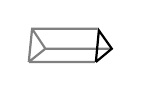
\begin{tikzpicture}[x=1.2em, y=1.2em]
    \draw[thick, black!50]
        (0,0)--(2,0)
        (2.075,1)--(0.1,1)--(0,0)
        (0,0)--(0.5,0.4)--(0.1,1)
        (0.5,0.4)--(2.5,0.4);
	\draw[thick] (2.02,0)--(2.5,0.4)--(2.11,0.95)--(2.02,0);
    \end{tikzpicture}
	 & A \\
	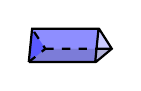
\begin{tikzpicture}[x=1.2em, y=1.2em,baseline=0.5em]
    \begin{scope}[thick]
    \fill[fill=blue, opacity=0.3]
        (0,0)--(2,0)--(2.1,1)--(0.1,1)--(0,0);
    \fill[fill=blue!50!black, opacity=0.3]
        (0,0)--(0.5,0.4)--(2.5,0.4)--(2,0)--(0,0);
    \fill[fill=blue, opacity=0.2]
        (0.1,1)--(0.5,0.4)--(2.5,0.4)--(2.1,1)--(0.1,1);
    \fill[fill=blue, opacity=0.5]
        (0.1,1)--(0.5,0.4)--(0,0)--(0.1,1);
    \draw
        (0,0)--(2,0)--(2.1,1)--(0.1,1)--(0,0)
        (2.02,0)--(2.5,0.4)--(2.117,1.001)
        (2.05,0.4)--(2.5,0.4);
    \draw[dashed]
        (0,0)--(0.5,0.4)--(0.1,1)
        (0.5,0.4)--(2.05,0.4);
    \end{scope}
    \end{tikzpicture}
    & X \\
	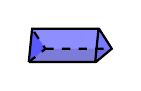
\begin{tikzpicture}[x=1.2em, y=1.2em,baseline=0.5em]
    \begin{scope}[thick]
    \fill[fill=blue, opacity=0.3]
        (0,0)--(2,0)--(2.1,1)--(0.1,1)--(0,0);
    \fill[fill=blue!50!black, opacity=0.3]
        (0,0)--(0.5,0.4)--(2.5,0.4)--(2,0)--(0,0);
    \fill[fill=blue, opacity=0.2]
        (0.1,1)--(0.5,0.4)--(2.5,0.4)--(2.1,1)--(0.1,1);
    \fill[fill=blue, opacity=0.5]
        (0.1,1)--(0.5,0.4)--(0,0)--(0.1,1);
    \fill[fill=blue, opacity=0.4]
        (2,0)--(2.5,0.4)--(2.1,1);
    \draw
        (0,0)--(2,0)--(2.1,1)--(0.1,1)--(0,0)
        (2.02,0)--(2.5,0.4)--(2.117,1.001);
    \draw[dashed]
        (0,0)--(0.5,0.4)--(0.1,1)
        (0.5,0.4)--(2.5,0.4);
    \end{scope}
    \end{tikzpicture}
	\arrow["{\bigcup\psi}", from=1-1, to=1-2]
	\arrow[from=1-1, to=2-1]
	\arrow[from=2-1, to=3-1]
	\arrow["{\psi_f}"', from=3-1, to=2-2]
	\arrow["\lambda"', dashed, from=2-1, to=1-2]
\end{tikzcd}
}
}
    \begin{tikzcd}[column sep=huge]
    (\de\ns\times e_1) \arrow[r, "\bigcup_{i=0,\dots,n} \psi_{d_i^*(f)}"] \arrow[d, hook] & A \arrow[d, hook] \\
    (\ns\times e_0)\cup(\de\ns\times\sx{1}) \arrow[ur, dashed, swap, "\lambda"] \arrow[r, swap, "\til f"] & X
    \end{tikzcd}
\end{center}

We reparametrize the relative homotopy into the desired map $\psi_f$ as follows:
\begin{center}
    \begin{tikzcd}
    (\ns\times e_0)\cup(\de\ns\times\sx{1})\times[0,1] \arrow[d] \arrow[r, "H"] & X \\
    \ns\times\sx{1} \arrow[ur, dashed, swap, "\psi_f"]
    \end{tikzcd}
\end{center}
considering the continuous quotient map.

The following picture illustrates the reparametrization for the $n=1$ case.

\smallskip
\begin{center}
    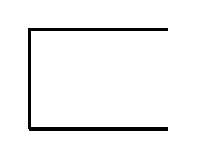
\begin{tikzpicture}[x=5em, y=1.2em,baseline=0.5em]
    \draw[very thick] (0,0)--(1,0) (1,3)--(0,3)--(0,0);
    \end{tikzpicture} \hspace{2em}
    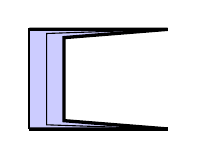
\begin{tikzpicture}[x=5em, y=1.2em,baseline=0.5em]
    \draw[very thick] (0,0)--(1,0) (1,3)--(0,3)--(0,0);
    \def\n{8}
    \def\t{2}
    \def\m{1/\n}
    \foreach \i in {\t,...,0}{
        % the first point is (x, x)
        % the second one is (x, 3-x)
        \filldraw[fill=blue!20] (0,0)--(1,0)--(\i*\m,\i*\m)--(\i*\m, 3-\i*\m)--(1,3)--(0,3);
    }
    \draw[very thick] (0,0)--(1,0)--(\t*\m,\t*\m)--(\t*\m, 3-\t*\m)--(1,3)--(0,3);
    \end{tikzpicture} \hspace{2em}
    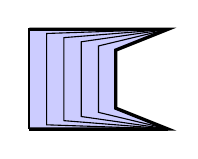
\begin{tikzpicture}[x=5em, y=1.2em,baseline=0.5em]
    \draw[very thick] (0,0)--(1,0) (1,3)--(0,3)--(0,0);
    \def\n{8}
    \def\t{5}
    \def\m{1/\n}
    \foreach \i in {\t,...,0}{
        % the first point is (x, x)
        % the second one is (x, 3-x)
        \filldraw[fill=blue!20] (0,0)--(1,0)--(\i*\m,\i*\m)--(\i*\m, 3-\i*\m)--(1,3)--(0,3);
    }
    \draw[very thick] (0,0)--(1,0)--(\t*\m,\t*\m)--(\t*\m, 3-\t*\m)--(1,3)--(0,3);
    \end{tikzpicture} \hspace{2em}
    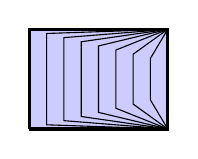
\begin{tikzpicture}[x=5em, y=1.2em,baseline=0.5em]
    \filldraw[very thick, fill=blue!20] (0,0)--(1,0)--(1,3)--(0,3)--(0,0);
    \def\n{8}
    \foreach \i in {0,...,\n}{
        \def\m{1/\n}
        % the first point is (x, x)
        % the second one is (x, 3-x)
        \draw (1,0)--(\i*\m,\i*\m)--(\i*\m, 3-\i*\m)--(1,3);
    }
    \end{tikzpicture}
\end{center}

\bigskip

Now we \enquote{adjoin} the continuous maps $\psi_f$ into the simplicial deformation retraction
\[H:\S(X)\times\Delta[1]\to \S(X),\]

that is, in the simplicial dimension $n$, we need to specify a map
\[\S(X)_n\times\Delta([n],[1])\to \S(X)_n.\]

We do this via an adjunction bijection:
\begin{multline*}
    \Hom_\sSet(Z\times\Delta[1],\S(X))\cong\\
    \cong\cb{\psi=\cb{\psi_z:\nabla^n\times\nabla^1\to X\text{ for all } n\geq0,\ z\in Z_n}\mid\psi_{\alpha^*(z)}=\psi_z\circ(\alpha_*  \times\id_{\nabla^1})}
\end{multline*}

\textit{Sketch} (full argument as an exercise).

Step 1. Given $H:Z\times\Delta[1]\to Y$ and $z\in Z_n$, we define $\psi^H_z:\Delta[n]\times\Delta[1]\to Y$ by
\[(\psi_z)_m(\alpha,\kappa)=H_m(\alpha^*(z),\kappa),\]
and using the Yoneda lemma we can show that the assignment $H\mapsto\cb{\psi^H_z}$ is bijective.

Step 2. $\S:\Top\to\sSet$ is right adjoint to $|-|:\sSet\to\Top$. This is AT1Sheet3.1

Step 3. There is a preferred homeomorphism $|\Delta[n]|\cong\ns$ given by
\[(\alpha:[m]\to[n],t)\mapsto\alpha_*(t),\text{ with inverse }s\mapsto[\id_{[n]},s],\] and the map
\[|\Delta[n]\times\Delta[1]|\xto{(|\pr_1|,|\pr_2|)}|\Delta[n]|\times|\Delta[1]|\cong\ns\times\sx{1}\]
is a homeomorphism. This is AT1Sheet3.2.

Step 4. Combine steps 1-3.
\begin{align*}
    \Hom_\sSet(Z\times\Delta[1],\S(X))&\underset{\text{Step 1}}{\cong}\cb{\cb{\psi_z:\Delta[n]\times\Delta[1]\to\S(X)\text{ for all } n\geq0,\ z\in Z_n}\mid\cdots}\\
    &\underset{\text{Step 2}}{\cong}\cb{\cb{\psi_z^\#:|\Delta[n]\times\Delta[1]|\to X}\mid\cdots}\\
    &\underset{\text{Step 3}}{\cong}\cb{\cb{\hat\psi_z:\ns\times\sx{1}\to X}\mid\cdots}
\end{align*}

\end{proof}

%%% Lecture 6

\section{Proof of Hurewicz Theorem}

\lecture[Hurewicz theorem at last! Then some generalities about fibre bundles.]{2021-11-3}

\begin{proof}[Proof of the Hurewicz theorem (\ref{theorem:hurewicz})]
We modify the definition of $\pi_n(X,A)^\#$ by replacing $\pair$ by the homeomorphic pair $(\ns,\de\ns)$.

Then the fundamental class $i\in H_n(\ns,\de\ns;\Z)$ is represented by the map $\id_\ns\in\S(\ns)_n$. The inclusion of simplicial sets (the $\cong$ comes from theorem \ref{theorem:simplicial-deformation-retraction} of last lecture)
\[\S(A)\into\S(X,A,n-1)\xinto{\cong}\S(X)\]
induces morphisms of chain complexes
\[C(\S(A))\to C(\S(X,A,n-1))\xto{\sim}C(\S(X))\]
where \enquote{$\sim$} is a chain homotopy equivalence.

We compare the long exact homology sequences:
\begin{center}
    \small
    \begin{tikzcd}
    \cdots \arrow[r] & H_n(A) \arrow[d, eq] \arrow[r] & H_n(C(\S(X,A,n-1))) \arrow[d, "\cong"] \arrow[r] & H_n(\frac{C(\S(X,A,n-1))}{C(\S(A))}) \arrow[d,"\cong \text{ (by 5-lemma!)}"] \arrow[r,"\de"] & \cdots \\
    & H_n(A) \arrow[r] & H_n(X) \arrow[r] & H_n(\frac{C(\S(X))}{C(\S(A))})=H_n(X,A) \arrow[r, "\de"] & \cdots
    \end{tikzcd}
\end{center}

Conclusion: the inclusion $\S(X,A,n-1)\into\S(X)$ induces an isomorphism
\[H_n\left(\frac{C(\S(X,A,n-1))}{C(\S(A))}\right)\xto{\cong} H_n(X,A)\]
so that we reduced the problem to finding an isomorphism
\[\pi_n(X,A)^\#\xto{``\cong"} H_n\left(\frac{C(\S(X,A,n-1))}{C(\S(A))}\right)\]

We note that $\S(X,A,\ni)_\ni=\S(A)_\ni$ so
\[\left(\frac{C(\S(X,A,n-1))}{C(\S(A))}\right)_\ni=0\]
which implies
\begin{align*}
    H_n(X,A)&\cong H_n\left(\frac{C(\S(X,A,n-1))}{C(\S(A))}\right) \\
    &=\coker\left(\frac{\Z[\S(X,A,\ni)_{n+1}]}{\Z[\S(A)_{n+1}]}\xto{\quad d\quad} \frac{\Z[\S(X,A,\ni)_n]}{\Z[\S(A)_n]}\right) \\
    &=\Z[f:(\ns,\de\ns)\to (X,A)]/E''
\end{align*}
where $E''$ is the subgroup generated by:
\begin{itemize}[label={-}]
    \item the classes of all $f:(\ns,\de\ns)\to(X,A)$ with $f(\ns)\subset A$,
    \item elements of the form $\sum_0^{n+1}(-1)^id_i^*(g)$ for all $g:\sx{n+1}\to X$ with $g(\sk_\ni(\sx{n+1}))\subset A$.
\end{itemize}

On the other hand, $\pi_n(X,A)^\#=\Z[f:(\ns,\de\ns)\to\pairs]/E'$
where $E'$ is generated by:
\begin{itemize}[label={-}]
    \item $f-f'$ for all pair homotopic $f\sim f'$,
    \item $f_1+f_2-(f_1\oplus f_2)$ whenever $f_1$ and $f_2$ are "addible".
\end{itemize}

To add maps on simplices of the same dimension, we divide $\ns$ into two sub-simplices by a procedure defined inductively, using the hyperplane $T^n$ in $\ns$ through $e_0$ and the hyperplane $T^{n-1}$ dividing $d_0(\sx{n})$. Pictured below, the $n=2$ case, starting with $T^1=\sum \frac{1}{2} e_i$.
\input{Pictures/Lec6Pic1}

Claim. The canonical homomorphism
\[\Z[f:(\ns,\de\ns)\to\pairs]\to \pi_n\pairs^\#,\quad [f]\mapsto[f]\]
factors through a homomorphism
\[\Phi: H_n\left(\frac{C(\S(X,A,n-1))}{C(\S(A))}\right)\to\pi_n\pairs^\#\]
(which is equivalent to saying that $E''\subset E'$).

\begin{claimproof}
We need to show that the two kinds of relations that generate $E''$ are sent to $0$.
\begin{itemize}[label={-}]
    \item If $f:(\ns,\de\ns)\to\pairs$ has image in $A$, we contract $\ns$ onto $e_0$ and postcompose this contraction homotopy with $f$. The result is a pair homotopy from $f$ to a constant map with value $f(e_0)$. So $[f]=[\const_{f(e_0)}]$, which is the zero element in $\pi_n\pairs^\#$.
    \item Now we consider all maps $g:\sx{n+1}\to X$ with $g(\sk_\ni(\sx{n+1}))\subset A$. We want to show that $\sum_0^{n+1}(-1)^i [g\circ(d_i)_*]=0$ in $\pi_n\pairs^\#$.
\end{itemize}

We consider the space $B=\sx{n}\cup_{\sx{n-1}}\dots\cup_{\sx{n-1}}\sx{n}$. It is a quotient space of a disjoint union of $n+2$ copies of $\ns$. If we number these copies from $0$ to $n+1$, we glue the $i$-th copy to the $(i+1)$-st copy by the maps:
\begin{center}
    \begin{tikzcd}
    \sx{\ni} \arrow[d,"(d_i)_*"] \arrow[r,"(d_i)_*"] & \ns_{((i+1)\text{-st})} \\
    \ns_{(i\text{-th})}
    \end{tikzcd}
\end{center}

Informally, $B$ is $\de\sx{n+1}$ "cut open", as shown in the following picture.
\input{Pictures/Lec6Pic2}
\smallskip
We define $p:B\to\de\sx{n+1}$ by defining the restriction to the $i$-th copy of $\ns$ as $(d_i)_*$. The map $p$ is compatible with the equivalence relation (and hence well defined on $B$) thanks to the simplicial relations:
\[d_i\circ d_i=d_{i+1}\circ d_i\]
The upshot is that $p$ is a quotient map onto $\de\sx{n+1}$.

Since $g$ is defined on all of $\sx{n+1}$, its restriction to $\de\sx{n+1}$ represents the $0$ element in $\pi_n\pairs^\#$.

\[\ns\cong B\xto{p}\de\sx{n+1}\into\sx{n+1}\xto{g}X.\]
\begin{center}
    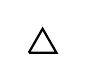
\begin{tikzpicture}[x=1em, y=1em]
        \draw[thick] (0,0)--(1,0)--(.5,.866)--(0,0);
    \end{tikzpicture}
    $\cong$
    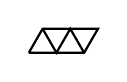
\begin{tikzpicture}[x=1em, y=1em]
        \draw[thick] 
        (0,0)--(2,0)--(2.5,.866)--(.5,.866)--(0,0)
        (.5,.866)--(1,0)--(1.5,.866)--(2,0);
    \end{tikzpicture}
    $\xto{p}$
    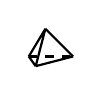
\begin{tikzpicture}[x=.2em, y=.2em, z=-.07em, baseline=0em]
    \draw[thick, black, dashed] 
        (-3,0,0) -- (5,0,0);
    \draw[thick, black]
        (5,0,0)--(0,5,0)
        (0,0,5)--(5,0,0)
        (0,5,0)--(0,0,5)
        (-3,0,0)--(0,5,0)
        (0,0,5)--(-3,0,0);
    \end{tikzpicture}
    $\into$
    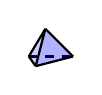
\begin{tikzpicture}[x=.2em, y=.2em, z=-.07em, baseline=0em]
    \draw[thick, black, dashed] 
        (-3,0,0) -- (5,0,0);
    \fill[fill=blue, opacity=0.3]
        (5,0,0)--(0,5,0)--(0,0,5)--(5,0,0);
    \fill[fill=blue, opacity=0.2]
        (-3,0,0)--(0,5,0)--(0,0,5)--(-3,0,0);
    \draw[thick, black]
        (5,0,0)--(0,5,0)
        (0,0,5)--(5,0,0)
        (0,5,0)--(0,0,5)
        (-3,0,0)--(0,5,0)
        (0,0,5)--(-3,0,0);
    \end{tikzpicture}
    $\xto{g} X.$
\end{center}


We apply the homotopy addition theorem (in simplex version) for the maps $\nno{f}{n+1}:\sx{n}\to B=\sx{n}\cup_{\sx{n-1}}\dots\cup_{\sx{n-1}}\sx{n}$, where $f_i$ is the inclusion of the $i$-th copy.
By the HAT:
\leftnote{\begin{center}
\begin{tikzpicture}[x=1em, y=1em]
\draw[thick] 
    (0,4)--(2,4)--(2.5,4.866)--(.5,4.866)--(0,4)
    (.5,4.866)--(1,4)--(1.5,4.866)--(2,4);
\draw[thick]
    (-4,2)--(-3,2)--(-3.5,2.866)--(-4,2)
    (-4,4)--(-3,4)--(-3.5,4.866)--(-4,4)
    (-4,6)--(-3,6)--(-3.5,6.866)--(-4,6);
\path[draw, -{\tip}, use Hobby shortcut,closed=false]
    (2,5.1) .. (2.5,5.7) .. (3.7,6);
\path[draw, -{\tip}] (-2.5, 2.5) -- (-0.5,4);
\path[draw, -{\tip}] (-2.5, 4.5) -- (-0.5,4.5);
\path[draw, -{\tip}] (-2.5, 6.1) -- (-0.5,5);
\path[draw, -{\tip}] (3, 4.5) -- (5,4.5);
\draw
    (-2,5.1) node{$f_i$}
    (4,3.8) node{$g|_{B}$}
    (2.5,6.6) node{$g|_{\cup\de\sx{n}}$}
    (3.8,6) node[anchor=west] {$A$}
    (5.2,4.5) node[anchor=west] {$X$};
\end{tikzpicture}
\end{center}
}
\[0=[g|_{\de \sx{m+1}}\circ p]=\sum_{i=0}^{m+1}(-1)^i[g\circ (d_i)_*].\]
% should this    ^    be an n? I think so

\end{claimproof}

Let's finish once and for all the proof:
\[H_n\left(\frac{C(\S(X,A,n-1))}{C(\S(A))}\right)\xto{\Phi}\pi_n(X,A)^\#\xto{h^\#}H_n(X,A;\Z)\]
the composite $h^\#\circ\Phi$ is the homomorphism induced by the inclusion $\S(X,A,n-1)\hto \S(X)$, which is an isomorphism. So $\Phi$ is injective. But $\Phi$ is also surjective since it hits all generators. So $\Phi$ is an isomorphism, hence $h^\#$ is an isomorphism.
\end{proof}



\chapter{Fibre Bundles and Fibrations}

\section{Generalities on Fibre Bundles}

A \textbf{fibre bundle} over a space $B$ is a continuous map $\pi:E\to B$ that is locally trivial in the following sense: for every point $b\in B$ there is a space $F$, a neighbourhood $U\subset B$ of $b$ and a homeomorphism such that the following diagram commutes:
\begin{center}
    \begin{tikzcd}
    \pi^{-1}(U) \arrow[dr,"\pi"] \arrow[rr,"\cong"] && U\times F \arrow[dl,"\pr_1"]\\
    & U
    \end{tikzcd}
\end{center}

$B$ is called the \textbf{base}, $E$ the \textbf{total space}, $F$ is the \textbf{fibre}, $\pi$ is the \textbf{projection}, the maps $\pi^{-1}(U)\xto{\cong} U\times F$ the \textbf{local trivialisations}.

If we fix $F$, the set of points $b\in B$ such that $F_b=\pi^{-1}(b)$ is homeomorphic to $F$ is open. So in particular, if $B$ is connected, then all fibres are homeomorphic.

\begin{examples}

Trivial fiber bundles: $\pi=\pr_1:E=B\times F\to B$.

Covering spaces: locally trivial fibre bundle with discrete fiber.

Vector bundles: particular fibre bundles with fibre $\R^n$.

Hopf fibration: $\eta:S^3\to S^2$.

\end{examples}

\begin{remark}

Suppose $\pi:E\to B$ is a locally trivial fibre bundle with fibre $\R^n$. For it to be a \textbf{vector bundle} there must be:
\begin{itemize}[label={-}]
    \item additional structure, as each fibre $F_b=\pi^{-1}(b)$ is given the structure of an $\R$ vector space,
    \item  additional conditions, i.e. the local trivialisation $\pi^{-1}(U)$ are fiberwise linear isomorphisms.
\end{itemize}

An equivalent perspective is the following. Suppose we chose a cover of $B$ by open subsets $\cb{U_i}_{i\in I}$ and local trivializations for each $U_i$, $u_i:\pi^{-1}(U_i)\xto{\cong} U_i\times\R^n$. For each pair of indices $i,j$ the "change of charts"
\[(U_i\cap U_j)\times\R^n\xto{u_i^{-1}}\pi^{-1}(U_i\cap U_j)\xto{u_j}(U_i\cap U_j)\times\R^n\]
is a homeomorphism on the projection to the first factors. So $\Phi=u_j\circ u_i^{-1}$ is of the form
\[(u_j\circ u_i^{-1})(x,v)=(x,\Psi(x,v))\]
for some map $\Psi:(U_i\cap U_j)\times\R^n\to\R^n$. The map $\Phi$ is adjoint to a function
\[U_i\cap U_j\to\homeo(\R^n,\R^n), x\mapsto\Psi(x,-)\]
In a vector bundle, the map factors through $\GL_n(\R)$, the linear automorphisms of $\R^n$.

Several related concepts/refinements of fibre bundles can also be conveniently formulated this way, by specifying a \textbf{structure group}, for example there is a hierarchy:
\begin{itemize}
    \item locally trivial fibre bundles with structure group $\homeo(\R^n,\R^n)$,
    \item smooth bundles with structure group $\diffeo(\R^n,\R^n)$,
    \item vector bundles with structure group $\GL_n(\R^n)$,
    \begin{itemize}
        \item vector bundles can be equipped with an inner product, in which case the structure group is required to be $\text{O}(n)$, 
    \end{itemize}
    \item oriented bundles with structure group $\GL_n^+(\R^n)$,
    \begin{itemize}
        \item oriented vector bundles can be equipped with an inner product, in which case the structure group is required to be $\text{SO}(n)$.
    \end{itemize}
\end{itemize}

\end{remark}

%%% Lecture 7

\section{Hopf Fibration}

\lecture[We construct the thing on the background of Schwede's homepage (Hopf fibration) and we introduce the long exact sequence associated to a fiber bundle (we also use our new toys to compute $\pi_3(S^2)$).]{2021-11-8}

The goals of the following two lectures (which are given by Markus Hausmann, a PhD student of Schwede) are:
\begin{enumerate}
    \item to construct the \textbf{Hopf fibration}, a fibre bundle $\eta:S^3\to S^2$ with fibre $S^1$,
    \item to associate to every fibre bundle $p:E\to B$ a long exact sequence of the form
    \[\cdots\to\pi_n(p^{-1}(b),e)\xto{i_*}\pi_n(E,e)\xto{p_*}\pi_n(B,b)\to\pi_\ni(p^{-1}(b),e)\to\cdots\]
\end{enumerate}

When we are done, we will have as a corollary the computation of our first \textit{really} non-trivial homotopy group.

\begin{corollary}
For every $n\geq 3$ there is an isomorphism $\pi_n(S^3,*)\cong\pi_n(S^2,*)$. In particular, $\pi_3(S^2,*)\cong\Z$, generated by the class of the Hopf fibration.
\end{corollary}

\begin{proof}
For $n\geq3$ we have
\[\cdots\to\pi_n(S^1,*)=0\to\pi_n(S^3,*)\xto{\eta_*}\pi_n(S^2,*)\to\pi_\ni(S^1,*)=0\to\cdots\]
which yields the claim.

In particular, for $n=3$ we get that $\eta_*:\pi_3(S^3,*)\cong\Z\to\pi_3(S^2,*)$ is an isomorphism which sends $[\id_{S^3}]$, generator of $\pi_3(S^3,*)$, to $[\eta\circ\id_{S^3}]=[\eta]$.
\end{proof}

The Hopf fibration is part of a family of fibre bundles. Let $K=\R$ or $\CC$ and recall the projective spaces:
\[\kpn=(K^{n+1}\sm\cb{0})/K^\times\]
where $x\sim\lambda x$ for all $x,\lambda\in K^\times$. In particular, we have that $\rpn$ is an $n$-dimensional manifold and $\cpn$ a $2n$-dimensional manifold. Moreover, recall that $\rp{1}\cong S^1$ and $\cp{1}\cong S^2$.

We consider now the projections $p:K^{n+1}\sm\cb{0}\to\kpn$.

Let $G$ be a topological group. A \tbf{principal $G$-bundle}\label{definition:principal-g-bundle} is a $G$-space $E$ such that:
\begin{numerate}
    \item for every $e\in E$ the map $G\to Ge=\cb{ge\mid g\in G}$, $g\to ge$, is a homeomorphism,
    \item the quotient map $p:E\to E/G=E/\sim$, where $e\sim ge$ for all $e\in E$, $g\in G$, is a fibre bundle.
\end{numerate}

\begin{example}
If we consider the real line (with the standard topology) with the group action of the additive group of the real numbers with the discrete topology, $\R_\delta\times\R\to\R$, this is an example of a $G$-space with a free action which does not satisfy property (1).
\end{example}

\begin{proposition}
 For $K=\R$ or $\CC$, the $K^\times$ action on $K^{n+1}\sm\cb{0}$ is a $K^\times$-principal bundle.
\end{proposition}

\begin{proof}
Let $e\in K^{n+1}\sm\cb{0}$. Then the map
\[K^\times\to K^\times e,\ \ \lambda\mapsto\lambda e\]
is continuous and satisfies $\|\lambda_1 e-\lambda_2 e\|=|\lambda_1-\lambda_2|\|e\|$. It follows that the inverse is also continuous.

It remains to show that $K^{n+1}\sm\cb{0}\to \kpn$ is a locally trivial fibre bundle. For $1\leq i\leq n+1$ let $X_i\subset K^{n+1}\sm\cb{0}$ be the subspace of tuples $(x_1,\dots,x_{n+1})$ such that $x_i\neq 0$, i.e. $x_i\in K^\times$. Then $K^{n+1}\sm\cb{0}=\cup_{i=1}^{n+1}X_i$. Let $Y_i=p(X_i)\subset \kpn$. This is open since $p^{-1}(Y_i)=X_i$. We define $u:p^{-1}(Y_i)=X_i\to Y_i\times K^\times$ by $u(x)=(p(x),x_i)$, with inverse
\[u^{-1}([x],\lambda)=(x_1/x_i,\dots,x_{i-1}/x_i,\lambda,x_{i+1}/x_i,\dots,x_{n+1}/x_i).\]
\end{proof}

For $K=\CC$ and $n=1$ this gives a fibre bundle
\[p:\CC^2\sm\cb{0}\cong S^3\to \cp{1}\cong S^2\]
with fibre $\CC^\times\cong S^1$. This is already the Hopf fibration \enquote{up to homotopy}.

Let $S(K^n)\subset K^n$ be the unit sphere ($(n-1)$-dimensional if $K=\R$, $(2n-1)$-dimensional if $K=\CC$). Further, let $G(K)\subset K^\times$ be the subgroup of elements of norm $1$ ($G(\R)=\cb{\pm1}$, $G(\CC)=S^1$). Then the $K^\times$-action on $K^{n+1}\sm\cb{0}$ restricts to a $G(K)$-action on $S(K^{n+1})$ and the induced map
\begin{center}
    \begin{tikzcd}
    S(K^{n+1})\arrow[r]\arrow[dr] & K^{n+1}\sm\cb{0}\arrow[r] & \kpn \\
    & S(K^{n+1})/G(K)\arrow[ur,swap,"\cong"]
    \end{tikzcd}
\end{center}
is a homeomorphism.

\begin{proposition}
The $G(K)$-action on $S(K^{n+1})$ defines a $G(K)$-principal bundle with base space $\kpn$.
\end{proposition}

\begin{proof}
Let $X_i\subset K^{n+1}\sm\cb{0}$, $Y_i\subset \kpn$ as before. We obtain a homeomorphism
\[v:q^{-1}(Y_i)=S(K^{n+1})\cap X_i\to Y_i\times G(K),\ \ x\mapsto (q(x),x_i/|x_i|).\]
\end{proof}

For $K=\R$ we obtain the covering space $S^n\to\rpn$ we already knew.

For $K=\CC$ we get a fibre bundle $S^{2n+1}\to\cpn$ with fibre $S^1$. For $n=1$ we get the Hopf fibration $\eta:S^3\to S^2$.

\begin{remark}
The Hopf fibration decomposes $S^3$ as a disjoint union of circles, continuously indexed over $S^2$.
It can be shown that any two of them are linked!

Considering $\eta:S^3\to S^2$ and $x_1\neq x_2\in S^2$
\[s:\eta^{-1}(x_1)\times\eta^{-1}(x_2)\to S^2,\ (x,y)\to\frac{x-y}{||x-y||}\]
is continuous. Choosing orientations on $S^2$ and $\eta^{-1}(x_1)\times\eta^{-1}(x_2)\cong S^1\times S^1$, we can consider the mapping degree of $s$. This is an example of an invariant for links called the \textbf{linking number} and it will be $\pm1$ in this case.
\end{remark}\smallskip

%\rightnote{Xiaoxiang Zhou suggested \href{https://www.youtube.com/watch?v=yNpqLMpfxA8&list=PL3C690048E1531DC7&index=7}{Dimension: a walk through mathematics} for an animation of the Hopf fibration.}

\begin{center}\rightnote{Someday I'll really wrap my head around this picture... (but maybe it's just not \textit{that} illuminating?)}
    \includegraphics[scale=0.45]{Pictures/HopfFibration.jpg}
\end{center}

\section{The Long Exact Sequence Associated to a Serre Fibration}

We turn now to our second goal. If $p:E\to B$ is a fibre sequence, $b\in B$, $e\in p^{-1}(b)$, then we want to show that there is a long exact sequence of the form:
\[\cdots\to\pi_n(p^{-1}(b),e)\to\pi_n(E,e)\to\pi_n(B,b)\to\pi_{n-1}(p^{-1}(b),e)\to\cdots\]

\begin{example}
Let $p:E\to B$ be a covering space. We get a long exact sequence (assuming $E$ is connected):
\[\cdots\to\pi_n(p^{-1}(b),e)=0\to\pi_n(E,e)\to\pi_n(B,b)\to\pi_\ni(p^{-1}(b),e)=0\to\cdots\]
\[\cdots\to 0 \to\pi_1(E,e)\to\pi_1(B,b)\to\pi_0(p^{-1}(b),e)\to 0\]

This amounts to the already known statements that $p_*:\pi_1(E,e)\to\pi_1(B,b)$ is injective (and that the fiber can be identified with the set of cosets of $p_*\pi_n(E,e)$ in $\pi_1(B,b)$) and that $p_*:\pi_n(E,e)\to\pi_n(B,b)$ is an isomorphism for $n\geq 2$. Both facts are usually proven using the lifting properties of covering spaces.\rightnote{There was a brief reminder on map lifting here.}
\end{example}

Let $p:E\to B$ be a continuous map. A \textbf{test situation} for the homotopy lifting property (HLP) consists of a space $X$ and a commutative square:
\begin{center}
    \begin{tikzcd}
    X \arrow[d,"i_0"'] \arrow[r,"f"] & E \arrow[d,"p"] \\
    X\times[0,1] \ar[ur,dashed,"\til H"'] \arrow[r,"H"'] & B
    \end{tikzcd}
\end{center}

A solution to the test situation is a map $\til H:X\times[0,1]\to E$
 such that $p\circ\til H=H$ and $\til H\circ i_0=f$.
 
there is also a relative version: a pair of spaces $\pairs$ and a commutative diagram:
\begin{center}
    \begin{tikzcd}
    X\times\cb{0}\cup(A\times[0,1]) \arrow[d, hook,"i_0"'] \arrow[r,"f"] & E \arrow[d,"p"] \\
    X\times[0,1] \ar[ur,dashed,"\til H"'] \arrow[r,"H"'] & B
    \end{tikzcd}
\end{center}

A solution is again a map $\til H:X\times[0,1]\to E$ such that $p\circ\til H=H$ and $\til H\circ i_0=f$.

A map $p:E\to B$ is called a \textbf{Hurewicz fibration} if it has the HLP with respect to every $X$ and all absolute test-situations for $X$.

A map $p:E\to B$ is called a \textbf{Serre fibration} if it has the HLP with respect to every CW-complex $X$ and all absolute test-situations for $X$.

For the proof of the existence of the long exact sequence associated to a fibre bundle we need two intermediate results.

\begin{proposition**}
Let $p:E\to B$ be a Serre fibration, $Y\subset B$ a subspace and $x\in p^{-1}(Y)$. Then the projection induces an isomorphism (for $n\geq 1$):
\[p_*:\pi_n(E,p^{-1}(Y),x)\xto{\cong}\pi_n(B,Y,p(x))\]
\end{proposition**}

\begin{corollary**}
Let $Y=\cb{b}$. We get a long exact sequence:
\[\cdots\to\pi_n(p^{-1}(b),x)\to\pi_n(E,x)\to\pi_n(E,p^{-1}(b),x)\cong\pi_n(B,b)\to\cdots\]
\end{corollary**}

\begin{theorem**}
Every fiber bundle is a Serre fibration.
\end{theorem**}

%%% Lecture 8

\lecture[We actually prove the story about the long exact sequence associated to a fibre bundle.]{2021-11-10}

Before we get to the promised results, we prove an auxiliary one.\rightnote{\Attention\ Didn't sleep much the night before this one, I hope I didn't type anything too stupid!}

\begin{lemma}\label{lemma:equivalent-HCP}
Let $p:E\to B$ be a map. The following are equivalent:
\begin{numerate}
\item $p$ is a Serre fibration,
\item $p$ has the absolute HLP for $D^n$ for all $n$,
\item $p$ has the relative HLP for $(D^n,\de D^n)$ for all $n$,
\item $p$ has the relative HLP for all relative CW-complexes.
\end{numerate}
\end{lemma}

\begin{proof}

$(1)\implies(2)$ This is true because $D^n$ is a CW-complex.

$(2)\implies(3)$ The space pairs $(D^n\times[0,1],D^n\times\cb{0})$ and $(D^n\times[0,1],D^n\times\cb{0}\cup\de D^n\times[0,1])$ are homeomorphic, hence any test situation for one HLP can be translated into a test situation for the other, and similarly for the solutions.

$(3)\implies(4)$ Let $(X,X')$ be a relative CW-complex. Consider the test situation:
\begin{center}
    \begin{tikzcd}
    X\times\cb{0}\cup X'\times[0,1] \arrow[d] \arrow[r,"f"] & E \arrow[d,"p"] \\
    X\times[0,1] \arrow[r] & B
    \end{tikzcd}
\end{center}

We first assume that $X=X'\cup_{\de D^n}D^n$ is obtained from $X'$ by attaching a single cell, with characteristic map $\alpha:D^n\to X$.

We obtain:

\begin{center}
    \begin{tikzcd}[row sep=huge]
    D^n\times\cb{0} \cup\de D^n\times[0,1] \arrow[d] \arrow[r] & X\times\cb{0} \cup X'\times[0,1] \arrow[d] \arrow[r,"f"] & E \arrow[d,"P"] \\
    D^n\times[0,1] \arrow[urr,dashed,crossing over,shift right,"H'"] \arrow[r,swap,"\alpha\times\id_{[0,1]}"] & X\times[0,1] \arrow[r,swap,"H"] & B
    \end{tikzcd}
\end{center}

By assumption, there exists a lift $H'$ as in the diagram.

Then the desired solution is
\[X\times[0,1]=(X'\times[0,1])\cup_{\de D^n\times[0,1]}D^n\times[0,1]\xto{f\cup H'}E.\]

The case where $(X,X')$ has finitely many relative cells follows by induction, the infinite case by passing to the colimit.

$(4)\implies(1)$ This is the special case $(X,\emptyset)$.
\end{proof}

\begin{remark}
CW-complexes are colimits of their skeleta.

\begin{center}
    \begin{tikzcd}
    \sk_n X\times[0,1] \arrow[r] \arrow[d,hook] & E \\
    \sk_{n+1}X\times[0,1] \arrow[ur,]
    \end{tikzcd}
\end{center}

We have
\[X\cong\colim_n\sk_n X\]
and since\rightnote{This is the first instance of the fact (which we will use very often) that \href{http://nlab-pages.s3.us-east-2.amazonaws.com/nlab/show/adjoints+preserve+(co-)limits}{adjoints preserve (co-)limits}.} the results in theorem \ref{theorem:exponential-law} assure us that the endofunctor $-\times Z$ of $\Top$ is a left adjoint (to the \enquote{exponentiation} functor; this is AT1Sheet11.2), we have
\[X\times[0,1]\cong\colim_n(\sk_n X\times[0,1]).\]
\end{remark}

Now we can prove the results promised at the end of last lecture.

\begin{lemma}
Let $p:E\to B$ be a Serre fibration, $Y\subset B$ and $x\in p^{-1}(Y)$. Then $p$ induces an isomorphism
\[p_*:\pi_n(E,p^{-1}(Y),x)\xto{\cong}\pi_n(B,Y,p(x))\]
for all $n\geq1$.
\end{lemma}

\begin{proof}
Surjectivity. Let $[\beta]\in\pi_n(B,Y,p(x))$ be represented by $\beta:(I^n,\de I^n,s_0)\to(B,Y,p(x))$ with $s_0=(0,\dots,0)$.
\begin{center}
    \(
    \begin{tikzcd}
    
\begin{tikzpicture}[x=2em, y=2em, baseline=0.7em]
        \draw[very thick, black!30] (0,0)--(1,0)--(1,1)--(0,1)--(0,0);
        \filldraw (0,0) circle (2pt);
    \end{tikzpicture}
    \ar[r, hook]\ar[d]
    & 
    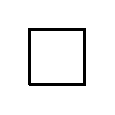
\begin{tikzpicture}[x=2em, y=2em, baseline=0.7em]
        \draw[very thick] (0,0)--(1,0)--(1,1)--(0,1)--(0,0);
    \end{tikzpicture} 
    \ar[r, hook]\ar[d]
    &
    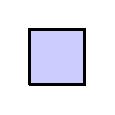
\begin{tikzpicture}[x=2em, y=2em, baseline=0.7em]
        \filldraw[very thick, fill=blue!20] (0,0)--(1,0)--(1,1)--(0,1)--(0,0);
    \end{tikzpicture}
    \ar[d]\\
    p(x)\ar[r, hook]&Y\ar[r, hook]&B
    \end{tikzcd}
    \)
\end{center}

To find a map $(I^n,\de I^n,s_0)\to(E,p^\inv(Y),x)$ mapped to $\beta$ by $p_*$, we would want to lift a homotopy of $\beta|_{I^\ni\times\cb{0}}$, as $\beta$ already looks like one. However, we cannot do this right away, because we are missing a lift of $\beta|_{I^\ni\times\cb{0}}$ to $E$. An obvious way to go about this is by repeated applications of the HLP, but since we are working with a contractible space, there is an easier and faster way.

Applying the HEP first to the relative CW-complex $(\de I^n,I^\ni\times\cb{0})$ for maps to $Y$, second for the relative CW-complex $\pair$ for maps to $B$, we can replace $\beta$ by an homotopic map $\beta'$ which sends all of $I^\ni\times\cb{0}$ to $p(x)$.

\input{Pictures/Lec8Pic2}

Now, the constant map $c_{p(x)}:I^\ni\times\cb{0}\to Y$ can be lifted to E via the constant map $c_x:I^\ni\times\cb{0}\to p^{-1}(Y)$, hence we have a test situation:
\begin{center}
    \begin{tikzcd}[column sep=large]
    I^\ni\times\cb{0} \arrow[d] \arrow[r,"c_x"] & E \arrow[d,"p"] \\
    I^n \arrow[r,swap,"\beta'"] \arrow[ur,dashed,"\exists\til\beta"] & B
    \end{tikzcd}
\end{center}
Since $p$ is a Serre fibration, there exists $\til\beta:I^n\to E$ such that $\til\beta|_{I^\ni\times\cb{0}}=c_x$, so that $\til\beta(s_0)=x$, and $p\circ\til\beta=\beta'$, so that $\til\beta(\de I^n)\subset p^{-1}(Y)$. Hence $\til\beta$ represents an element $[\til\beta]$ of $\pi_n(E,p^{-1}(Y),x)$, which by construction maps to $[\beta']=[\beta]$ under $p_*$.

Injectivity. Let $\alpha_1,\alpha_2:(I^n,\de I^n,s_0)\to(E,p^{-1}(Y),x)$ represent elements of $\pi_n(E,p^{-1}(Y),x)$ which are sent to the same element under $p_*$. Then there exists a homotopy of triple maps $H:I^n\times I\to B$ from $p\circ\alpha_1$ to $p\circ\alpha_2$.

\[
\begin{tikzcd}[column sep = huge]
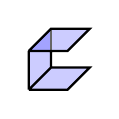
\begin{tikzpicture}[x = 1.4em, y = 1.4em, z = 0.8em, baseline = 0.4em]
    \begin{scope}[fill=blue, opacity=0.2]
    \fill
    (0,0,0) -- (0,1,0) -- (0,1,1) -- (0,0,1) -- (0,0,0);
    \fill
    (0,0,0) -- (1,0,0) -- (1,0,1) -- (0,0,1) -- (0,0,0);
    \fill
    (0,1,0) -- (1,1,0) -- (1,1,1) -- (0,1,1) -- (0,1,0);
    \end{scope}
    \begin{scope}[thick]
    \draw[black!60]
    (0,0.4,1) -- (0,1,1);
    \draw
    (0,0,1) -- (0,0.45,1)
    (0,0,0) -- (0,1,0)
    (0,0,0) -- (1,0,0) -- (1,0,1) -- (0,0,1) -- (0,0,0)
    (0,1,0) -- (1,1,0) -- (1,1,1) -- (0,1,1) -- (0,1,0);
    \end{scope}
\end{tikzpicture}
\ar[r, "\alpha_1\cup c_x\cup\alpha_2"] \ar[d] & E \ar[d, " p"]\\
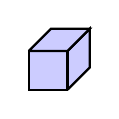
\begin{tikzpicture}[x = 1.4em, y = 1.4em, z = 0.8em, baseline = 0.4em]
    \begin{scope}[fill=blue!20, thick]
    \filldraw
    (1,0,0) -- (1,1,0) -- (1,1,1) -- (1,0,1) -- (1,0,0);
    \filldraw
    (1,0,0) -- (1,1,0) -- (0,1,0) -- (0,0,0) -- (1,0,0);
    \filldraw
    (0,1,0) -- (1,1,0) -- (1,1,1) -- (0,1,1) -- (0,1,0);
    \end{scope}
\end{tikzpicture}
\ar[r, "H"'] \ar[ur, dashed] & B
\end{tikzcd}\rightnote{Note that for this to work we have to \enquote{swap} the last two coordinates!}
\]

Again we can assume that $\alpha_1(I^\ni\times\cb{0})=\alpha_2(I^\ni\times\cb{0})=\cb{x}$. In addition we can assume that $H$ sends $(I^\ni\times\cb{0})\times I$ constantly to $p(x)$. We again lift $c_{p(x)}$ to $c_x$ and view $\alpha_1$ and $\alpha_2$ as lifts of $H$ on the subspace $I^\ni\times\cb{0}\times\cb{0}\cup I^\ni\times\cb{0}\times\cb{1}$. Since $(I^\ni\times\cb{0}\times I,I^\ni\times\cb{0}\times\cb{0}\cup I^\ni\times\cb{0}\times\cb{1})$ is a relative CW-complex, we can apply the relative HLP to lift $H$ to a map $\til H:I^n\times I\to E$, giving a relative homotopy from $\alpha_1$ to $\alpha_2$.
\end{proof}

We remember that this has as a consequence the long exact sequence associated to a Serre fibration.

\begin{theorem}
Let $Y=\cb{b}$, $F=p^{-1}(b)$. We get a long exact sequence:
\[\cdots\to\pi_n(F,x)\to\pi_n(E,x)\to\pi_n(E,F,x)\cong\pi_n(B,b)\to\cdots\]
\end{theorem}

Many examples of Serre fibrations come from fibre bundles, thanks to the next theorem.

\begin{theorem}
Every fibre bundle is a Serre fibration.
\end{theorem}

\begin{proof}
Let $p:E\to B$ be a fibre bundle and a lifting problem
\begin{center}
    \begin{tikzcd}
    X\times\cb{0} \arrow[r,"f"] \arrow[d] & E \arrow[d,"p"] \\
    X\times I \arrow[r,"H"] & B
    \end{tikzcd}
\end{center}

Easy case. Let $p$ be globally trivial, i.e. of the form $\pr_B:B\times F\to B$ for some space $F$. Then we have
\begin{center}
    \begin{tikzcd}[column sep=large]
    X\times\cb{0} \arrow[r,"{(f_1, f_2)}"] \arrow[d] & B\times F \arrow[d,"\pr_B"] \\
    X\times I \arrow[r,swap,"H"] \arrow[ur,dashed,"\til H"] & B
    \end{tikzcd}
\end{center}
We can define a lift $\til H$ explicitly via $\til H(x,t)=(H(x,t),f_2(x))$ (this works for any space $X$).

General case. We have to glue local lifts together systematically.

By lemma \ref{lemma:equivalent-HCP}, it suffices to check the HLP for disks $D^n$, or equivalently for cubes $I^n$. Hence we are given:
\begin{center}
    \begin{tikzcd}
    I^n\times\cb{0} \arrow[r,"f"] \arrow[d] & E \arrow[d,"p"] \\
    I^n\times I \arrow[r,"H"] & B
    \end{tikzcd}
\end{center}

Let $\cb{U_i}_{i\in I}$ be an open covering of $B$, such that $p^{-1}(U_i)\xto{p}U_i$ is a trivial fibre bundle for all $i$. Pulling back along $H$, we get an open cover of $I^n\times I$. By Lebesgue's lemma, we can divide $I^n\times I$ into smaller cubes of side length $1/k$, such that each cube is contained in some $p^{-1}(U_i)$.\rightnote{The drawing is an explanation of how \enquote{row by row}               is fine and otherwise not: this is because the HLP lets us lift the \enquote{base} of the little cubes (or some more, in the relative case), but in the situation pictured on the right there is no way to be sure that our lifting will coincide with the map we already have in the upper side of the cube.}
\input{Pictures/Lec8Pic3}\medskip

We can then extend $H$ iteratively over the smaller cubes \enquote{row by row}. In every situation this amounts to choosing a solution to the relative lifting problem for a globally trivial fibre bundle.
\end{proof}

\begin{remark}
Not every fibre bundle is a Hurewicz fibration (but actual counter-examples are complicated). A sufficient condition is that the base space be paracompact.
\end{remark}

\begin{remark}

An interesting question: are liftings of homotopies unique? It turns out that they are unique up to homotopy! Indeed, let $\til H_1$ and $\til H_2$ two liftings of an homotopy $H$, then we can apply the HLP to obtain a homotopy between them: 
\begin{center}
    \begin{tikzcd}[column sep=huge]
    X\times\cb{0} \arrow[r] \arrow[d] & E \arrow[d,"p"] \\
    X\times I \arrow[r,"H"'] \arrow[ur,dashed,"\til H_1", "\til H_2"'] & B
    \end{tikzcd}\qquad
    \begin{tikzcd}[column sep=huge]
    X\times I\times\cb{0} \cup X\times I\times\cb{1} \arrow[r,"\til H_1\cup\til H_2"] \arrow[d] & E \arrow[d,"p"] \\
    X\times I\times I \ar[ur,dashed,shift right=1] \arrow[r,"\const_H"'] & B
    \end{tikzcd}
\end{center}\normalmarginpar
\end{remark}

%%% Lecture 9

\section{More on Fibre Bundles and Fibrations}

\lecture[Some more fibre bundles/fibrations stuff. Prof. Schwede suggests that we take the categorical red pill. Shout-out to the category of compactly generated spaces (without definition). We introduce the compact-open topology.]{2021-11-15}

Prof. Schwede is back!

\begin{theorem}
Let $p:E\to B$ be a continuous map, with path-connected base.
\begin{numerate}
    \item If $p$ is a Hurewicz fibration, then any two fibers of $p$ are homotopy equivalent.
    \item If $p$ is a Serre fibration, then any two fibres which are CW-complexes are homotopy equivalent.
\end{numerate}
\end{theorem}

\begin{proof}
Let $b_0,b_1\in B$ be points, set $F_0=p^{-1}(b_0),F_1=p^{-1}(b_1)$.

Let $\omega:[0,1]\to B$ be a path from $b_0$ to $b_1$. Choose homotopies $H$ and $K$ as liftings in the followings diagrams:
\begin{center}
\begin{tikzcd}[column sep=large]
F_0\times 0 \arrow[r,"\incl"] \arrow[d,hook] & E \arrow[d,"p"] \\
F_0\times[0,1] \arrow[ur,dashed,"H"] \arrow[r,"\omega\circ\pr_2"] & B
\end{tikzcd}\qquad
\begin{tikzcd}[column sep=large]
F_1\times 0 \arrow[r,"\incl"] \arrow[d,hook] & E \arrow[d,"p"] \\
F_1\times[0,1] \arrow[ur,dashed,"K"] \arrow[r,"\bar\omega\circ\pr_2"] & B
\end{tikzcd}
\end{center}

where $\bar\omega(t)=\omega(1-t)$ is the inverse path.

We set $f=H(-,1):F_0\to F_1$ and $g=K(-,1):F_1\to F_0$.

Let $L:[0,1]\times[0,1]\to B$ be a homotopy, relative $\cb{0,1}$, from the concatenated path $\omega*\bar\omega$ to $\const_{b_0}$.
\[L(-,0)=\omega*\bar\omega,\]
\[L(-,1)=\const_{b_0}\]
\[L(0,t)=L(1,t)=b_0\]

Choose another lifting in the following diagram:

\begin{center}
    \begin{tikzcd}[column sep=huge]
    F_0\times((0\times I)\cup(I\times 0)\cup(1\times I)) \arrow[r] \arrow[d,hook] & E \arrow[d,"p"] \\

    F_0\times[0,1]\times[0,1] \arrow[ur,dashed,swap,"\bar L"] \arrow[r,swap,"L\circ\pr_{2,3}"] & B
    \end{tikzcd}
\end{center}
where the upper arrow is\alvaropls\ $(\const_{\incl}\,\cup\, H*(K\circ(f\times\id))\,\cup\,\const_{\incl\circ 
g\circ f})$.\smallskip

\begin{center}
    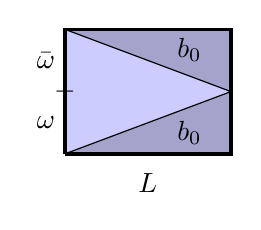
\begin{tikzpicture}[x=1.5em, y=1.5em, baseline=2.1em]
    \filldraw[very thick, fill=blue!20] (0,0)--(0,3)--(4,3)--(4,0)--(0,0);
    \draw (0,0)--(4,1.5)--(0,3);
    \filldraw[fill = black, opacity = 0.2] (0,0)--(4,1.5)--(0,3)--(4,3)--(4,0)--(0,0);
    \filldraw
    (0,.75) node[anchor=east]{$\omega$}
    (0,2.25) node[anchor=east]{$\bar\omega$}
    (0,1.5) node {$-$}
    (3,2.5) node {$b_0$}
    (3,0.5) node {$b_0$}
    (2,-0.7) node{$L$};
    \end{tikzpicture}
    \hspace{2cm}
    \(\displaystyle
    \begin{tikzcd}[column sep=huge]
    F_0\times
        
\begin{tikzpicture}[x=1em, y=1em, baseline=0.2em]
        \draw[very thick] (0,1)--(0,0)--(1,0)--(1,1);
        \end{tikzpicture}
    \arrow[r] \arrow[d,hook] & E \arrow[d,"p"] \\
    F_0\times
        
\begin{tikzpicture}[x=1em, y=1em, baseline=0.2em]
        \filldraw[very thick, fill=blue!20] (1,0)--(0,0)--(0,1)--(1,1)--(1,0);
        \end{tikzpicture}
    \arrow[ur,dashed,swap,"\bar L"] \arrow[r,swap,"L\circ\pr_{2,3}"] & B
    \end{tikzcd}\)
\end{center}

\vspace{-0.1cm}
Then we can set $G=\bar L(-,-,1):F_0\times[0,1]\to E$ to obtain a homotopy from $\incl:F_0\into E$ to $\incl\circ\,g\circ f:F_0\to E$.

Since $p\circ G=\const_{b_0}$, this homotopy $G$ takes place inside $F_0$. So $G$ can be seen as a homotopy from $\id_{F_0}$ to $g\circ f$. Reversing the roles of $b_0$ with $b_1$, $F_0$ with $F_1$ and $f$ with $g$ yields a homotopy from $\id_{F_1}$ to $f\circ g$.
\end{proof}

\unnumpar{Induced fibres bundles/fibrations}

We construct the pullback bundle\rightnote{This construction is also called base change sometimes. Or fiber product.}. Let $p:E\to B$ and $\beta:B'\to B$ be continuous maps. The pullback is \[E'=B'\times_B E=\cb{(b',e)\in B'\times E\mid \beta(b')=p(e)}\]
with subspace topology of the product topology.

\begin{center}
    \begin{tikzcd}
    &[-6ex] (b',e) \arrow[r,mapsto] & e \\[-4ex]
    (b',e) \arrow[d,mapsto] & B'\times_B E \arrow[d,dashed,"p'"] \arrow[r,dashed,"\beta'"] & E \arrow[d,"p"] \\
    
    b' & B' \arrow[r,"\beta"] & B
    \end{tikzcd}
\end{center}

This is a pullback in $\Top$ in the sense of category theory, i.e. the following universal property holds: for all spaces $A$ and continuous maps $\alpha:A\to B'$ and $\epsilon:A\to E$ such that $\beta\alpha=p\epsilon$, there is a unique continuous map $\delta:A\to B'\times_B E$ such that $\beta'\delta=\epsilon$ and $\alpha\delta=p'$, namely the map $\delta(a)=(\alpha(a),\epsilon(a))$.
\begin{center}
    \begin{tikzcd}
    A \arrow[dr,dashed,"\exists!\delta"] \arrow[drr,bend left,"\epsilon"] \arrow[ddr,bend right,"\alpha"] & & \\
     & B'\times_B E \arrow[d,"p'"] \arrow[r,"\beta'"] & E \arrow[d,"p"] \\
    
     & B' \arrow[r,"\beta"] & B
    \end{tikzcd}
\end{center}

\begin{example}[Restriction bundle]
Suppose $B'$ is a subspace of $B$ and $\beta:B'\to B$ the inclusion. Then we have
\[B'\times_B E\cong p^{-1}(B')\]
with homeomorphisms given by
\[(b',e)\mapsto e,\]
\[(p(e),e)\mapsfrom e.\]
\end{example}

\begin{example}[A pretty stupid one]
I lost the explanation, but take it as a little rebus:
\begin{center}
    \begin{tikzcd}
    B'\amalg B' \arrow[d] \arrow[r] & B' \arrow[d] \\
    *\amalg* \arrow[r] & *
    \end{tikzcd}
\end{center}
\end{example}
In general taking the constant map $\beta:B'\to B$ to a point $b\in B$ will yield as the pullback bundle the trivial bundle $B'\times p^{-1}(b)$.

\begin{theorem}
Let $p:E\to B$ and $\beta:B'\to B$ be continuous maps.
\begin{itemize}
    \item[(i)] If $p$ is a fibre bundle, then so is $p':B'\times_B E\to B'$.
    \item[(ii)] If $p$ is a Hurewicz fibration, then so is $p'$.
    \item[(iii)] If $p$ is a Serre fibration, then so is $p'$.
\end{itemize}
\end{theorem}

\begin{proof}\rightnote{\emph{\enquote{You take the blue pill — the story ends, you wake up in your bed and believe whatever you want to believe. You take the red pill — you stay in Wonderland, and I show you how deep the rabbit hole goes.}}}There's two reasonable proofs of the first fact, one direct, one categorical. The Professor seems to be suggesting a blue pill/red pill situation (with the categorical version being \emph{\enquote{much more transparent}} to him).

(i) Consider any point $a\in B'$. There is a open neighbourhood $U$ of $\beta(a)$ in $B$ and a local trivialization, i.e. a homeomorphism $\psi:p^{-1}(U)\to U\times F$ for one space $F$ (over $U$).

We argue that $p':B'\times_B E\to B'$ is trivializable over $V=\beta^{-1}(U)$ with the same fibre $F$.

The following are mutually inverse homeomorphisms:
\begin{align*}
    (p')^{-1}(V)&\xleftrightarrow{\ \cong\ }V\times F\\
    (b',e)&\ \,\mapsto\ (b',\psi_2(e))\\
    (b',\psi^{-1}(\beta(b'),f))&\ \,\mapsfrom\ (b',f).
\end{align*}

Categorical proof: the statement is an instance of the fact that \enquote{pullbacks are transitive}.

In any category $\Cc$, we consider a commutative diagram:
\begin{center}
    \begin{tikzcd}[column sep={8em,between origins}]
    B''\times_B E \arrow[d] \arrow[r] & B'\times_B E \arrow[d,"p'"] \arrow[r,"\beta'"] & E \arrow[d] \\
    
    B'' \arrow[r] & B' \arrow[r,"\beta"] & B
    \end{tikzcd}
\end{center}

If both squares are pullbacks, then the composite square is also a pullback. Symbolic notation:
\[B''\times_B E\cong B''\times_{B'}(B'\times_B E).\]

Hence, considering the same situation as in the direct proof, we have:
\[(p')^{-1}(V)\cong V\times_B E\cong V\times_{B'}(B'\times_B E)\cong V\times_U(U\times_B E)\cong V\times_U(U\times F)\cong V\times F.\]

(ii)+(iii) We show: whenever $p:E\to B$ has the HPL for some space $X$, then $p':B'\times_B E\to B'$ also has the HLP for $X$.

Consider a lifting square on the left:
\begin{center}
    \begin{tikzcd}[column sep=large,row sep=huge]
    X\times0 \arrow[d,hook] \arrow[r,"f"] & B'\times_B E \arrow[d,"p'" near end] \arrow[r,"\beta'"] & E \arrow[d,"p"] \\
    
    X\times[0,1] \arrow[ur,dashed,bend left=20,blue,"\til H"] \arrow[urr,dashed,crossing over,red, "K" near start] \arrow[r,"H"'] & B' \arrow[r,"\beta"'] & B
    \end{tikzcd}
\end{center}

There is a homotopy $K:X\times[0,1]\to E$ so that $p\circ K=\beta\circ H$ and $K(-,0)=\beta'\circ f$.

The universal property of the pullback provides a unique continuous map
\[\til H:X\times[0,1]\to B'\times_B E\]
such that $p'\circ \til H=H$ and $\beta'\circ\til H=K$.

The two continuous maps $f,\,\til H(-,0):X\times0\to B'\times_B E$ compose in the same way with $p'$ and with $\beta'$. The uniqueness part of the universal property then forces $f=\til H(-,0)$.
\end{proof}

\chapter{Mapping Spaces}

\section{Compact-open Topology}

Our aim: to define and study a specific topology on $Z^X=\cb{f:X\to Z\text{ continuous}}.$

We would like the "exponential law" to hold: the map
\begin{align*}
    Z^{X\times Y}&\to(Z^X)^Y\\
    (f:X\times Y\to Z)&\mapsto \cb{y\mapsto f(-,y)}
\end{align*}
should be a homeomorphism.

Unfortunately, it is not. At least not in general, but the good news is that it is whenever $Y$ is Hausdorff and $X$ locally compact.

\begin{remark}
There is a way to arrange the exponential law in complete generality: work in the full subcategory $CG$ of compactly generated spaces. Then $CG$ is a cartesian closed category, i.e. it has finite products and for all $X\in\operatorname{ob}(G)$
\[-\times X:CG\to CG\]
has a right adjoint, written $Z\mapsto Z^X$.

Watch out: the product in $CG$ is not always the usual product topology!

Some examples of classes of spaces in $CG$ are:
\begin{itemize}[label={-}]
    \item every locally compact Hausdorff space,
    \item every CW-complex,
    \item every manifold is in $CG$,
    \item the realization of every simplicial set,
    \item for two CW-complexes $X$ and $Y$, the product in $CG$, $X\times_{CG}Y$, is again a CW-complex.
    \item for all simplicial sets $A,B$, the canonical map:
    \[|A\times B|\to|A|\times_{CG}|B|\]
    is a homeomorphism.
\end{itemize}
\end{remark}

Enter: the compact-open topology. For spaces $X$ and $Z$, write $Z^X$ for the set of continuous maps $f:X\to Z$. Let $K$ be a compact subset of $X$ and let $O$ be an open subset of $Z$. Set:
\[W(K,O)=\cb{f\in Z^X:f(K)\subset O}\subset Z^X.\]

The \textbf{compact-open topology} on $Z^X$ is the topology generated by the sets $W(K,O)$ with $K\subset X$ compact and $O\subset Z$ open, i.e. these sets form a subbasis of the compact-open topology.

\begin{theorem}
Let $X$ be a compact space and $(Z,d)$ a metric space.
\begin{numerate}
\item There is a metric on $Z^X$, defined as:
\[d(g_1,g_2)=\sup_{x\in X}d(g_1(x),g_2(x)),\text{ for }g_1,g_2\in Z^X.\]
called the supremum metric.
\item The compact-open topology on $Z^X$ coincides with the metric topology of the supremum metric.
\end{numerate}
\end{theorem}

\begin{proof}
(1) Omitted (see \cite[proposition A.13]{hatcher}).

(2) \enquote{$\subset$}: compact-open is metrically open.

It suffices to show that the generating sets $W(K,O)$ are metrically open. Fix $K\subset X$ compact, $O\subset Z$ open and $f\in W(K,O)$, i.e. $f(K)\subset O$. Then $C=Z\sm O$ is a closed subset of $Z$ and $f(x)\not\in C$ for all $x\in K$ (hence $d(f(x),C)>0$ for all $x\in K$). Since $K$ is compact, $\epsilon=\inf_{x\in K}d(f(x),C)>0$
is positive.
We claim that $B_{\sup}(f,\epsilon)\subset W(K,O)$.

Let $g\in Z^X$ be such that $d(f,g)<\epsilon$. Then $d(f(x),g(x))<\epsilon$ for all $x\in K$, hence:
\[d(f(x),g(x))\leq d(f(x),C),\]
so $g(x)\in O=Z\sm C$. Therefore $g(K)\subset O$, so $g\in W(K,O)$.

\enquote{$\supset$}: metrically open is compact-open.

Let $A\subset Z^X$ be open in the sup-topology, $f\in A$. We will construct finitely many compact sets $K_i$ in $X$ and open sets $O_i$ in $Z$ so that:
\[f\in W(K_1,O_1)\cap\dots\cap W(K_m,O_m)\subset A.\]

Since $A$ is open in the sup-topology, there is an $\epsilon>0$ so that $A$ contains the $\epsilon$-ball around $f$.

For $x\in X$ the set $f^{-1}(B(f(x),\epsilon/5))$ is an open neighbourhood of $x$ in $X$. Since $X$ is compact\rightnote{Note: compact spaces, meaning quasi-compact \textit{and} Hausdorff, are locally compact, but quasi-compact spaces may not be!}, this contains a compact neighbourhood $K_x$ of $x$. Since $X$ is compact, there are finitely many $x_1,\dots,x_m$ such that $X=K_{x_1}\cup\dots\cup K_{x_m}$.
Set $K_i:=K_{x_i}$ and $O_i:=$ open $\epsilon/5$-neighbourhood of $f(K_i)$ in $Z$.

\input{Pictures/Lec9Pic2}
As shown in the picture, for all $z,z'\in O_i$, we have $d(z,z')\leq 4\epsilon/5<\epsilon$ (to expand on this, observe we have $f(K_x) \subset B(f(x),\frac{\varepsilon}{5})\subseteq O_x := \frac{\varepsilon}{5}\text{-neighborhood of }f(K_x)$, hence both $z$ and $z'$ are at distance less or equal than $\frac{\varepsilon}{5}$ from two points of $f(K_x)$, and both these points are at distance less or equal than $\frac{\varepsilon}{5}$ from $f(x)$).

Suppose that $g\in W(K_1,O_1)\cap\dots\cap W(K_m,O_m)$. Then for all $x\in X$ there is $1\leq i\leq m$ with $x\in K_i$. Since $g\in W(K_i,O_i)$, we have $g(x)\in O_i$. We also have $x\in K_i=K_{x_i}$, so $d(f(x),f(x_i))\leq\epsilon/5$ so $f(x)\in O_i$. Hence $d(g(x),f(x))<\epsilon$. Since this holds for all $x\in X$, $d(f,g)<\epsilon$. So $W(K_1,O_1)\cap\dots\cap W(K_m,O_m)\subset B_{\sup}(f,\epsilon)\subset A$.
\end{proof}

% Lecture 10

\lecture[Legend has it that if you repeat compact-open for two hours loop spaces will appear.]{2021-11-17}

I missed this lecture, thanks to Paul for providing photos of the blackboard!

Up to now we have proved the following facts:
\begin{itemize}[label={-}]
    \item for a Hurewicz fibration (resp. Serre fibration) over a path-connected space, the fibres are homotopy equivalent (resp. the same, but whenever they admit CW-structures),
    \item fibre bundles, Hurewicz fibrations and Serre fibrations are stable under base change,
    \item if $X$ is compact and $Z$ is a metric space, the compact-open topology on $Z^X$ agrees with the topology of the supremum metric.
\end{itemize}

\begin{example}
Let $I$ be any set, endowed with the discrete topology. Let $Z$ be a space and consider $Z^I=\prod_I Z$. Then the compact-open topology on $Z^I$ agrees with the product topology.
\begin{itemize}
    \item Let $J$ be any subset of I; then $J$ is compact if and only if it is finite. So the sets $W(J,O)=\prod_{j\in J}O\times\prod_{j\not\in J}Z$ for $J$ finite and $O$ open form a subbasis of the compact-open topology. These sets are open in the product topology.
    \item A subbasis in the product topology is given by the sets $\prod_{j\in J}O_j\times\prod_{j\not\in J}Z$ for $J\subset I$ finite and $O_j$ open in $Z$. But then we have that
    \[\prod_{j\in J}O_j\times\prod_{j\not\in J}Z=\bigcap_{j\in J}(O_j\times\prod_{i\neq j}Z)=\bigcap_{j\in J}W(\cb{j},O_j)\]
    is open in the compact-open topology.
\end{itemize}
\end{example}

\begin{theorem}\label{theorem:compact-subbasis-topology}
Let $X$ and $Z$ be spaces and let $\S$ be a subbasis of the topology on $Z$. Then the sets $W(K,O)$ for $K\subset X$ compact and $O\in\S$ form a subbasis of the compact-open topology.
\end{theorem}

\begin{proof}
The "new topology" (generated by $W(K,O)$ for $O\in\S$) is clearly contained in the compact-open topology. We need to show that for all $O\subset Z$ open, the set $W(K,O)$ is open in the new topology.

If $O\in\S$, this is true by definition.

If $O=\nns{O}{\cap}{n}$ with $O_i\in\S$, then
\[W(K,O)=W(K,O_1)\cap\cdots\cap W(K,O_n)\]
which is open in the new topology.

Now, suppose $O=\bigcup_{i\in I}O_i$ with $O_i\in\Bb$, where $\Bb$ is the basis generated by $\S$, i.e. the set of all finite intersections of sets in $\S$. Let $f\in W(K,O)$. Then for each $x\in K$ there is a set $O_x\in\Bb$ with $f(x)\in O_x\subset O$. Since $K$ is compact, hence locally compact, there is a compact neighbourhood $K_x$ of $x$ with $f(K_x)\subset O_x$. The covering $\cb{K_x}_{x\in K}$ of the compact set $K$ has a finite subcover $K\subset K_{x_1}\cup\cdots\cup K_{x_n}$. Then
\[f\in \bigcap_{i=1,\dots,n}W(K_{x_i},O_{x_i})\subset W(K,O).\]
\end{proof}

\begin{theorem}
Let $X$ and $Z$ be spaces and let $X$ be locally compact. Then the evaluation map $\ev:Z^X\times X\to Z,\ \ev(f,x)=f(x)$, is continuous.
\end{theorem}

\begin{proof}
Let $O$ be any open subset of $Z$. We want to show that
\[\ev^{-1}(O)=\cb{(f,x)\in Z^X\times X:f(x)\in O}\]
is open. Let $(f,x)\in Z^X\times X$ be in $\ev^{-1}(O)$, so $f(x)\in O$. Since $f$ is continuous, $f^{-1}(O)$ is an open neighbourhood of $x$. Since $X$ is locally compact, there is a compact neighbourhood $K$ of $x$ inside $f^{-1}(O)$. Then $f\in W(K,O)$ and $W(K,O)\times K$ is a neighbourhood of $(f,x)$ in $Z^X\times X$. Then $\ev(W(K,O)\times K)\subset O$, hence $(f,x)\in W(K,O)\times K\subset\ev^{-1}(O)$, so $\ev$ is continuous.
\end{proof}

\begin{theorem}\label{theorem:exponential-law}
Let $X,Y$ and $Z$ be spaces.
\begin{numerate}
    \setcounter{enumi}{-1}
    \item For every continuous map $f:X\times Y\to Z$, the adjoint map $\Phi(f):Y\to Z^X$ defined by $\Phi(f)(y)(x)=f(x,y)$ is continuous. So $\Phi$ defines a map $Z^{X\times Y}\to(Z^X)^Y$.
    \item The map $\Phi:Z^{X\times Y}\to(Z^X)^Y$ is continuous.
    \item If $X$ is locally compact (and Hausdorff), then $\Phi$ is bijective.\rightnote{\upshape Locally compact includes Hausdorff for Schwede.}
    \item If $X$ is locally compact and $Y$ is Hausdorff, then $\Phi$ is a homeomorphism.
\end{numerate}
\end{theorem}

\begin{proof}\ 

(0) Let $f:X\times Y\to Z$ be continuous and $\Phi(f):Y\to Z^X$ the adjoint map. To show that $\Phi(f)$ is continuous, it suffices to show that the sets $(\Phi(f))^{-1}(W(K,O))$ are open in $Y$ for all $K\in X$ compact, $O\in Z$ open. Let $y\in (\Phi(f))^{-1}(W(K,O))$, i.e. $f(K\times\cb{y})\subset O$, or $K\times\cb{y}\subset f^{-1}(O)$ which is open. By the \href{https://en.wikipedia.org/wiki/Tube_lemma}{tube lemma}, there is a open neighbourhood $U$ of $y$ in $Y$ such that $K\times U\subset f^{-1}(O)$ or equivalently $\Phi(f)(U)\subset W(K,O)$. Hence $y\in U\subset(\Phi(f))^{-1}(W(K,O))$, so the latter set is open in $Y$.

(1) The compact-open topology on $Z^X$ has a subbasis consisting of the sets $W(K,O)$ for $K\subset X$ compact and $O\subset Z$ open. By theorem \ref{theorem:compact-subbasis-topology} the compact-open topology on $(Z^X)^Y$ has a subbasis of the form $W(K',W(K,O))$ for $K\subset X$ compact, $K'\subset Y$ compact, $O\subset Z$ open. But $\Phi^{-1}(W(K',W(K,O)))=W(K\times K',O)$ which is open in the compact-open topology on $Z^{X\times Y}$ because $K\times K'$ is again compact.

(2) On the set-theoretic level, every map $Y\to Z^X$ is of the form $\Phi(f)$ for some unique map $f:X\times Y\to Z$. So $\Phi$ is continuous by (1) and injective. We have to show that when $X$ is locally compact and $g:Y\to Z^X$ is continuous, $\Phi^{-1}(g)$ is continuous. But since the evaluation map is continuous, by (0) the composite
\[\Psi(g):X\times Y\cong Y\times X\xto{g\times\id}Z^X\times X\xto{\ev}Z\]
is continuous and we have:
\[\Phi(\Psi(g))(y)(x)=\Psi(g)(x,y)=\ev(g(y),x)=g(y)(x)\text{ for all }x\in X,y\in Y,\]
so that $\Phi(\Psi(g))=g$, i.e. $\Psi(g)=\Phi^\inv(g)$.

(3) Now we suppose that $X$ is locally compact Hausdorff and $Y$ is Hausdorff. As we saw in (1), the sets $W(K',W(K,O))$ with $K\subset X$ and $K'\subset Y$ compact, $O\subset Z$ open, form a subbasis on $(Z^X)^Y$. Then
\[\Phi^{-1}(W(K',W(K,O)))=W(K\times K',O)\]
so that we just need to show that the sets $W(K\times K',O)$ generate the compact-open topology on $Z^{X\times Y}$. This is the content of the following lemma.
\end{proof}

\begin{lemma}
Let $X$ and $Y$ be Hausdorff spaces and $Z$ any space. Then the compact-open topology on $Z^{X\times Y}$ is generated by the sets $W(K\times K',O)$ for all $K\subset X$ compact, $K'\subset Y$ compact and $O\subset Z$ open.
\end{lemma}

\begin{proof}
Let $L$ be any compact subset of $X\times Y$ and $O$ an open subset of $Z$. We need to show that $W(L,O)$ is open in the potentially small topology generated by the sets $W(K\times K',O)$. Let $f\in W(L,O)$ be arbitrary, we have $L\subset f^{-1}(O)$, which is open in $X\times Y$. For each $(x,y)\in L$ we can choose $U_{x,y}$ open in $X$ and $V_{x,y}$ open in $V$ with $(x,y)\in U_{x,y}\times V_{x,y}\subset f^{-1}(O)$. We set $L_X=\pr_X(L)$ and $L_Y=\pr_Y(L)$, which are quasi-compact subsets of $X$ and $Y$ respectively. Since $X$ and $Y$ are Hausdorff, $L_X$ and $L_Y$ are indeed compact, hence locally compact. For each $(x,y)\in L$ we can find compact neighbourhoods $K_{x,y}$ of $x$ in $L_X$ and $K'_{x,y}$ of $y$ in $L_Y$. Then the sets $\cb{K_{x,y}\times K'_{x,y}}_{(x,y)\in L}$ cover L. Since $L$ is compact, there is a finite subcover $\cb{K_{x,y}\times K'_{x,y}}_{(x,y)\in I}$ with $I$ finite. Then
\[f\in\underbrace{\bigcap_{(x,y)\in I}W(K_{x,y}\times K'_{x,y},O)}_{\text{open in the new topology}}=W(\bigcup_{(x,y)\in I}K_{x,y}\times K'_{x,y},O)\subset W(L,O)\]
where the last inclusion follows from $L\subset \bigcup_{(x,y)\in I}K_{x,y}\times K'_{x,y}$.
\end{proof}

\begin{remark}
The assignment $(Z,X)\mapsto Z^X$ is a bifunctor
\[(-)^{(-)}:\Top\times\Top^\op_{H}\to \Top.\]

Contravariant functoriality: let $f:X\to X'$ be a continuous map between Hausdorff spaces. Define $f^*:Z^{X'}\to Z^X$ by precomposition with $f$, i.e.
\[f^*(\psi:X'\to Z)=\psi\circ f:X\to Z.\]

This map is continuous: let $K\subset X$ be compact, $O\subset Z$ open, then
\[(f^*)^{-1}(W(K,O))=\cb{\psi:X'\to Z\mid (\psi\circ f)(K)\subset O}=W(f(K),O).\]
Since $K$ is compact, $f(K)$ is quasi-compact; since $X'$ is Hausdorff, $f(K)$ is compact.

Covariant functoriality: let $g:Z\to Z'$ be continuous. We define $g_*:Z^X\to (Z')^X$ by postcomposition with $g$, i.e.
\[g_*(\psi:X\to Z)=g\circ\psi:X\to Z'.\]

This map is continuous: let $K\subset X$ be compact and $O\subset Z'$ open, then
\[g_*^{-1}(W(K,O))=\cb{\psi:X\to Z\mid (g\circ\psi)(K)\subset O}=W(K,g^{-1}(O)),\]
which is open in $Z^X$.

Note also that for $f:X\to X'$ continuous, $g:Z\to Z'$ continuous and $X,X'$ Hausdorff, the following square commutes:
\begin{center}
    \begin{tikzcd}
    (Z')^{X'} \arrow[r,"f^*"] & (Z')^X\\
    Z^{X'} \arrow[u,"g_*"] \arrow[r,"f^*"] & Z^X \arrow[u,"g_*"]
    \end{tikzcd}
\end{center}
\end{remark}

\begin{example}
Let $f,g:X\to Z$ be homotopic maps, with $H:X\times[0,1]\to Z$ a homotopy between them. The adjoint $\Phi(H):[0,1]\to Z^X$ is then continuous. Hence homotopies correspond to paths in $Z^X$, so that the map
\begin{align*}
[X,Z]&\to\pi_0(Z^X)\\
[f]\ \ &\mapsto\ \ [f]
\end{align*}
where $[X,Z]$ indicates the set of homotopy classes of maps $X\to Z$, is well-defined, surjective and a bijection whenever $X$ is locally compact.
\end{example}

\section{Path Spaces and Loop Spaces}

For a space $X$, the space $X^{[0,1]}$ is the \textbf{path space} of $X$. For a pointed space $(X,x_0)$, the \textbf{loop space} $\Omega X$ is the subspace of $X^{[0,1]}$ consisting of all loops at $x_0$, i.e. those $\omega\in X^{[0,1]}$ with $\omega(0)=\omega(1)=x_0$.

Let $q:[0,1]\to S^1=\cb{z\in\CC\mid|z|=1}$ be the quotient map $q(x)=e^{2\pi ix}$, this induces a continuous map
\[q^*:X^{S^1}\to X^{[0,1]},\]
which restricts to a continuous bijection onto $\Omega X$, considered as the space
\[(X,x_0)^{(S^1,1)}=\cb{f:S^1\to X\mid f(1)=x_0}.\]
This is in fact a homeomorphism, as a special case of the following lemma.

\begin{lemma}\label{lemma:quotient-map-induces-homeomorphism-on-mapping-spaces}
Let $q:X\to Y$ be a quotient map between compact spaces. Then for every space $Z$, the continuous map $q^*:Z^Y\to Z^X$ is a homeomorphism onto the subspace of all functions $f:X\to Z$ that factor through $q$.
\end{lemma}

% Lecture 11

\lecture[We continue studying mapping spaces.]{2021-11-22}

We prove the lemma from last lecture.\rightnote{\Attention\ I definitely still need to digest lecture 11 and 12, don't count on everything I write.}

\begin{proof}
First, note that $q^*$ is injective, continuous and has the desired image by the universal property of the quotient topology. We show that $q^*$ is also open as a map onto its image. We let $K\subset Y$ be compact and $O\subset Z$ be open. Then
\[q^*(W(K,O))=\cb{g\circ q:X\to Z\mid g\in Z^Y,\ g(K)\subset O}=W(q^{-1}(K),O)\cap\im(q^*).\]
Because $K$ is compact and $Y$ Hausdorff, $K$ is closed in $Y$; so $q^{-1}(K)$ is closed in $X$. Since $X$ is compact, $q^{-1}(K)$ is again compact. So $W(q^{-1}(K),O)\cap\im(q^*)$ is open.
\end{proof}

\begin{example}
The map $q:[0,1]\to S^1=\cb{z\in\CC:|z|=1}$, $q(x)=e^{2\pi ix}$ is a quotient map, so
\[q^*:X^{S^1}\to\cb{f\in X^{[0,1]}\mid f(0)=f(1)}\]
is a homeomorphism. For any base point $x_0\in X$, this homeomorphism restricts to a homomorphism
\[(X,x_0)^{(S^1,1)}\to\Omega X.\]

If $(Y,y_0)$ is a pointed space, the pointed version of $[Y,Z]=\pi_0(Z^Y)$ yields a well-defined surjective map $[Y,Z]_*\to\pi_0((Z,z_0)^{(Y,y_0))}$. If $Y$ is locally compact, this is a bijection.

For $Y=S^1$, this gives a bijection $\pi_1(Z,z_0)\cong\pi_0((Z,z_0)^{(S^1,1)})=\pi_0(\Omega Z)$.
\end{example}

\subsection{Loop Shifts the Homotopy Groups}

Let $(Y,y_0)$ be a based space. The reduced suspension is the space:
\[\Sigma Y=\frac{Y\times[0,1]}{Y\times 0\cup\cb{y_0}\times[0,1]\cup Y\times 1}.\]

The quotient map $q:Y\times[0,1]\to\Sigma Y$ induces a continuous injection:
\[q^*:(Z,z_0)^{(\Sigma Y,*)}\to Z^{Y\times[0,1]}\]
whose image consists of all continuous maps $f:Y\times[0,1]\to Z$ that factor through the quotient map, i.e. such that $f(Y\times 0\cup\cb{y_0}\times[0,1]\cup Y\times 1)=\cb{z_0}$. If $Y$ is compact, then so are $Y\times[0,1]$ and $\Sigma Y$, and $q^*$ is even an homeomorphism onto its image:
\[(Z,z_0)^{(\Sigma Y,*)}\cong(\Omega Z,\const_{z_0})^{(Y,y_0)}.\]

In particular:
\[\Hom_{\Top_*}((\Sigma Y,*),(Z,z_0))\cong\Hom_{\Top_*}((Y,y_0),(\Omega Z,\const_{z_0})).\]

So the functors $\Sigma$ and $\Omega$ are adjoint endofunctors in the category of based spaces.

On path components, we obtain a bijection
\[[\Sigma Y,Z]_*\cong[Y,\Omega Z]_*.\]

For $Y=S^n$ the last bijection specializes to a bijection
\[\pi_{n+1}(Z,z_0)=[S^{n+1},Z]_*\cong[\Sigma S^n,Z]_*\cong[S^n,\Omega Z]_*=\pi_n(\Omega Z,\const_{z_0})\]
which is even a group homomorphism (as we will see).

\section{Mapping Spaces and Serre Fibrations}

\begin{theorem}
Let $Z$ be any space, $(X,A)$ a relative CW-complex with $X$ and $A$ finite CW-complexes.\rightnote{\upshape A slightly more general statement was mentioned but I missed it. I guess $X$ and $A$ need not be finite but something weaker?} Then the restriction map $\incl^*:Z^X\to Z^A$, $f\mapsto f|_A$ is a Serre fibration.
\end{theorem}

\begin{proof}
We show that $\incl^*$ has the HLP with respect to all CW-complexes $Q$. So we consider a lifting diagram
\[\begin{tikzcd}
Q\times0 \arrow[d,hook] \arrow[r,"f"] & Z \arrow[d,"\incl^*"] \\
Q\times[0,1] \arrow[r,"\Phi"] & Z^A
\end{tikzcd}\]
Since $X$ and $A$ are locally compact we can use the exponential law to adjoint $f$ and $\Phi$ to continuous maps
\[\til f:X\times Q\times0\to Z\]
\[\til\Phi:A\times Q\times[0,1]\to Z\]
The condition $\incl^*\circ f=\Phi|_{Q\times0}$ becomes the relation that $\til f$ and $\til\Phi$ coincide on $A\times Q\times0$.

We consider the glued maps
\[\til f\cup\til\Phi:X\times Q\times 0\cup A\times Q\times[0,1]\to Z.\]

Since $(X\times Q,A\times Q)$ is a relative CW-complex, it has the HEP so there is a continuous extension $H:X\times Q\times[0,1]\to Z$ that extends $\til f$ and $\til\Phi$. The adjoint $H^\#:Q\times[0,1]\to Z^X$ of $H$ then solves the original lifting problem.
\end{proof}

For the relative CW-complex $([0,1],\cb{0,1})$ the theorem says that the restriction map
\[Z^{[0,1]}\to Z^{\cb{0,1}}\cong Z\times Z,\ w\mapsto (w(0),w(1))\]
is a Serre fibration for every space $Z$.

We let $z_0\in Z$ be any base point. Define $EZ$ as the subspace of $Z^{[0,1]}$ of all paths that start at $z_0$.

Equivalently, $EZ$ is the pullback:
\begin{center}
    \begin{tikzcd}
    w \ar[d,mapsto] &[-6ex] EZ \arrow[d] \arrow[r,hook] & Z^{[0,1]} \arrow[d] &[-6ex] w \ar[d,mapsto] \\
    w(1) & Z \arrow[r,"{(z_0,-)}"] & Z\times Z & (w(0),w(1))
    \end{tikzcd}
\end{center}

Since Serre fibrations are stable under base-change, we conclude that the map $EZ\to Z$, $w\mapsto w(1)$ is a Serre fibration.

\begin{theorem}\label{theorem:EZ-contractible}
The space $EZ$ is contractible onto the constant path at $z_0$.
\end{theorem}

\begin{proof}
Let $H:[0,1]\times[0,1]\to[0,1]$ be a homotopy, relative $\cb{0}$, that contracts the interval onto $0$, e.g. $H(s,t)=s(1-t)$. Let
\[H^*:Z^{[0,1]}\to Z^{[0,1]\times[0,1]}\]
be the continuous induced map and
\[\til H^*:Z^{[0,1]}\times[0,1]\to Z^{[0,1]}\]
its adjoint, i.e. $\til H^*(w,t)(s)=w(H(s,t))$.

We observe that
\[\til H^*(w,t)(0)=w(H(0,t))=w(0).\]
So whenever $w(0)=z_0$ (i.e. $w\in EZ$), then also $\til H^*(w,t)(0)=z_0$. In other words, for all $t\in[0,1]$, the map $\til H^*(-,t)$ takes $EZ$ to $EZ$. So we can restrict $\til H^*$ to a continuous map $\til H^*:EZ\times[0,1]\to EZ$; this is the desired contracting homotopy:
\[\til H^*(w,1)(s)=w(H(s,1))=w(0)\]
so the homotopy $\til H^*$ ends in the constant map at $z_0$.

For all $w\in EZ$, $\til H^*(w,0)(s)=w(t(s,0))=w(s)$, so $\til H^*(w,0)=w$.
\end{proof}

Now we can see that $\pi_n(\Omega,*)\cong\pi_{n+1}(Z,z_0)$ is a group morphism.

\begin{proof}[Second proof/construction of the isomorphism $\pi_n(\Omega Z,*)\cong\pi_{n+1}(Z,z_0)$]

We have seen that the space $EZ=\cb{w\in Z^{[0,1]}\mid w(0=z_0)}$ is contractible.

The map $e:EZ\to Z$, $e(w)=w(1)$ is a Serre fibration, so for every point in $Z$, we get a long exact sequence of homotopy groups. For $z_0\in Z$, the fibre of $e$ at $z_0$ is $\Omega Z$; hence the long exact sequence of homotopy groups is:
\[\dots\to\pi_{n+1}(EZ,*)=0\xto{e_*}\pi_{n+1}(Z,z_0)\xto{\de}\pi_n(\Omega Z,*)\xto{\incl_*}\pi_n(EZ,*)=0\to\cdots\]

So for $n\geq 1$, the connecting morphism $\de:\pi_{n+1}(Z,z_0)\to\pi_n(\Omega Z,*)$ is an isomorphism.
\end{proof}

\section{Turning Maps into Fibrations, up to Homotopy}

This is kind of dual to the mapping cylinder.

\begin{theorem}
Every continuous map $f:X\to Y$ can be factored functorially and naturally\todo[color=red]{ What does he mean by functorially and naturally?} as a composite
\[X\xto{\cong}Ef\xto{p} Y\]
of a homotopy equivalence followed by a Serre fibration.
\end{theorem}

\begin{proof}
Let $Ef=X\times_Y Y^{[0,1]}=\cb{(x,w)\in X\times Y^{[0,1]}\mid f(x)=w(0)}$. More precisely, $Ef$ is the pullback:
\[\begin{tikzcd}
Ef \arrow[d] \arrow[r] & Y^{[0,1]} \arrow[d] &[-6ex] w \ar[d,mapsto] \\
X \arrow[r,"f"] & Y & w(0)
\end{tikzcd}\]

We define natural continuous maps $h:X\to Ef$ by $h(x)=(x,\const_{f(x)})$ and $p:Ef\to Y$ by $p(x,w)=w(1)$.

Clearly we have $f=p\circ h$.

We observe that $Ef$ can be described as a slightly different pullback:
\[\begin{tikzcd}
(x,w) \ar[d,mapsto] &[-6ex] Ef \arrow[d] \arrow[r] & Y^{[0,1]} \arrow[d] &[-6ex] w \ar[d,mapsto]\\
(x,w(1)) & X\times Y \arrow[r,"f\times\id"] & Y\times Y & (w(0),w(1))
\end{tikzcd}\]

Since Serre fibrations are stable under base change, the map $Ef\to X\times Y$, $(x,w)\mapsto(x,w(1))$ is a Serre fibration. Since $\pr_2:X\times Y\to Y$ is a Serre fibration and Serre fibrations are closed under composition, $p$ is a Serre fibration. 
The map $h:X\to Ef$ is a homotopy equivalence: the homotopy inverse, which is also a left inverse, is the projection to the first factor.

Claim. The composite $c:Ef\to Ef$ is homotopic to the identity.

\begin{claimproof}
We define the desired homotopy
\[\bar H:Ef\times[0,1]\to Ef=X\times_Y Y^{[0,1]}\]
by specifying its projections to $X$ and to $Y^{[0,1]}$. The first coordinate of $\bar H$ is $Ef\times[0,1]\to X$, $(x,w,t)\mapsto x$, i.e. the constant homotopy of the projection to $X$. The second coordinate is the composite
\[Ef\times[0,1]\xto{\pr_2\times\id} Y^{[0,1]}\times [0,1]\xto{\til H^*} Y^{[0,1]}\]
where $\til H^*$ is the homotopy we constructed in the proof of theorem \ref{theorem:EZ-contractible}.

This has the following properties:
\begin{itemize}[label={-}]
    \item $\bar H$ starts with the identity,
    \item for all $t\in [0,1]$, all $w\in Y^{[0,1]}$, the path $\til H^*(w,t)$ has the same startpoint as $w$, so $\bar H$ really lands in $Ef$.
    \item $\til H^*(w,1)$ is constant at $w(0)$, which means that $\bar H(-,1)=h\circ\pr_1$.
\end{itemize}
\end{claimproof}
\end{proof}

% Lecture 12

\lecture[Homotopy fibre and the homotopy groups of a map (wew).]{2021-11-24}

The \textbf{homotopy fibre} of a continuous map $f:X\to Y$ over a point $y_0\in Y$ is the space:
\begin{align*}
    \ho_{y_0}(f)&=X\times_Y Y^{[0,1]}\times_Y \cb{y_0}\\
    &=\cb{(x,w)\in X\times Y^{[0,1]}\mid f(x)=w(0),w(1)=y_0}=p^{-1}(y_0).
\end{align*}

Informally the homotopy fibre is what we get when we turn the map into a Serre fibration, then take the actual fibre.

Because $p:Ef\to Y$ is a Serre fibration, the homotopy groups of $\ho_{y_0}(f)$ participate in a long exact sequence:
\[\cdots\to\pi_{n+1}(Y,y_0)\xto{\de}\pi_n(\ho_{y_0}(f),x)\to\pi_n(X,x)\xto{f_*}\pi_n(Y,y_0)\to\cdots\]

The slogan is: the homotopy fibres measure how far $f$ is from a real homotopy equivalence.

If $X$ and $Y$ happen to be path-connected CW-complexes, then $f$ is a homotopy equivalence if and only if $\pi_n(\ho_{y_0}(f),x)=0$ for all $n\geq0$.

For $f:X\to Y$ the analogy goes:

\begin{center}
\begin{tabular}{ m{6.5cm} | m{6.5cm} } 
 $Z(f)=X\times[0,1]\cup_{X\times1}Y$:
 & $Ef=X\times_Y Y^{[0,1]}$: \\ 
 \[\begin{tikzcd}[column sep=large]
    X \arrow[r,"\text{cl. emb.}"] \arrow[dr,"f"] & Z(f)\arrow[d,"(f \circ \pr_1)\cup\id_Y","\simeq"']\\
     & Y
    \end{tikzcd}\] & \[\begin{tikzcd}[column sep=large]
    X \arrow[r,"\sim"] \arrow[dr,"f"] & Ef\arrow[d,"p"]\\
     & Y
    \end{tikzcd}\] \\ 
 $Cf=Z(f)/X=*\cup_{X\times0}X\times[0,1]\cup_{X\times1} Y$. & $\ho_{y_0}(f)=X\times_Y Y^{[0,1]}\times_Y\cb{y_0}$. \\
  & \\
 Long exact homology sequence. & Long exact homotopy sequence.
\end{tabular}
\end{center}

Where the long exact homology sequence we are referring to is the one associated with the mapping cone:
\[\cdots\to H_n(X;A)\xto{f_*} H_n(Y;A)\to \til H_n(Cf;A)\xto{\de} H_\ni(X;A)\to\cdots\]
and the long exact homotopy sequence the one associated with the homotopy fibre.

\section{Relative Homotopy Groups of a Map}

Let $X,Y$ be spaces, $f:X\to Y$ a continuous map and $x_0\in X$, $y_0=f(x_0)$. Choose a basepoint $s_0\in S^{n-1}\subset D^n$.

Elements of the homotopy group $\pi_n(f)$ are represented by commutative squares of continuous maps:
\begin{center}
    \begin{tikzcd}
    (S^{n-1},s_0) \arrow[d,hook] \arrow[r,"\alpha"] & (X,x_0) \arrow[d,"f"] \\
    (D^n,s_0) \arrow[r,"\beta"] & (Y,y_0)
    \end{tikzcd}
\end{center}

Two representatives $(\alpha_0,\beta_0)$ and $(\alpha_1,\beta_1)$ define the same class in $\pi_n(f)$ when there is a commutative square of continuous maps
\begin{center}
    \begin{tikzcd}
    (S^{n-1},s_0)\times[0,1] \arrow[d,hook] \arrow[r,"H"] & (X,x_0) \arrow[d,"f"] \\
    (D^n,s_0)\times[0,1] \arrow[r,"\bar H"] & (Y,y_0)
    \end{tikzcd}
\end{center}
such that $H(-,0)=\alpha_0$, $H(-,1)=\alpha_1$, $\bar H(-,0)=\beta_0$, $\bar H(-,1)=\beta_1$.

If $X\subset Y$ and $f$ is the inclusion, then the map $\alpha$ is already defined by $\beta$, and it exists precisely when $\beta(S^\ni)\subset X$. So $\pi_n(\incl:X\into Y)=\pi_n(Y,X,x_0)$.

There is also an alternative (and isomorphic) description via cubes. We consider equivalence classes of commutative diagrams of continuous maps of pairs:
\begin{center}
    \begin{tikzcd}
    (I^\ni,\de I^\ni) \arrow[d,hook] \arrow[r,"\alpha"] & (X,x_0) \arrow[d,"f"] \\
    (I^n,J^\ni) \arrow[r,"\beta"] & (Y,y_0)
    \end{tikzcd}
\end{center}

The advantage of this description is that for $n\geq2$ we can define a group structure on $\pi_n(f)$ by stacking representatives next to each other in the first coordinate.

The long exact sequence of homotopy groups also generalizes:
\[\cdots\to\pi_{n+1}(f)\xto{\de}\pi_n(X,x_0)\xto{f_*}\pi_n(Y,y_0)\to\pi_n(f)\to\cdots\tag{$*$}\]

where $\de$ is:
\[[\alpha:S^n\to X,\beta:D^{n+1}\to Y]\mapsto\alpha,\]

and the map $\pi_n(Y,y_0)\to\pi_n(f)$ is:

\[[\beta:(I^n,\de I^n)\to(Y,y_0)]\mapsto
\begin{tikzcd}
(I^\ni,\de I^\ni) \arrow[d,hook] \arrow[r,"\const_{x_0}"] & (X,x_0) \arrow[d,"f"] \\
    (I^n,J^\ni) \arrow[r,"\beta"] & (Y,y_0)
\end{tikzcd}
.\]

The long exact sequence is natural in $f:X\to Y$, i.e. for every commutative square
\begin{center}
    \begin{tikzcd}
     X \arrow[d,"\phi"] \arrow[r,"f"] & Y \arrow[d,"\psi"] \\
    X' \arrow[r,"f'"] & Y'
    \end{tikzcd}
\end{center}
we get a commutative diagram of long exact sequences.

\begin{theorem}
The long exact sequence of homotopy groups $(*)$ is exact.
\end{theorem}

There are two possible proof, one "short", one instructive.

\begin{proof}\ 

1. Mimic the arguments for $\pi_n(Y,X,x_0)$, i.e. the special case $f=\incl:X\into Y$.

2. For $n\geq1$ there is a natural isomorphism $\pi_\ni(\ho_{y_0}(f),*)\cong\pi_n(f)$ such that the following diagram commutes:
\[
\begin{tikzcd}[column sep={8em,between origins},row sep=large]
& \pi_n(Y,y_0) \arrow[dl,"\de"'] \arrow[dr] & \\
\pi_\ni(\ho_{y_0}(f),*) \arrow[dr] \arrow[rr,"\cong"] && \pi_n(f) \arrow[dl,"\de"] \\
 & \pi_\ni(X,x_0) &
\end{tikzcd}
\]
where the connecting homomorphism on the top left of the diagram comes from the sequence of spaces $\ho_{y_0}(f)\into Ef\xto{p} Y$ and the map on the bottom left is induced by $\pr_1:\ho_{y_0}(f)\to X$.

Since the long exact sequence of the Serre fibration $p:Ef\to Y$ is exact, we have that the new sequence $(*)$ is also exact.

The isomorphism is constructed as follows.

$\ho_{y_0}(f)=X\times_Y Y^{[0,1]}\times_Y\cb{y_0}$, so elements of $\pi_\ni(\ho_{y_0}(f),*)$ are represented by continuous maps of pairs $\gamma:(I^\ni,\de I^\ni)\to (X\times_Y Y^{[0,1]}\times_Y\cb{y_0},*)$. The representative $\gamma$ consists of two continuous maps $\alpha:(I^\ni,\de I^\ni)\to(X,x_0)$ and $\bar\beta:(I^\ni,\de I^\ni)\to(Y^{[0,1]},\const_{y_0})$ that satisfy $f\circ\alpha=\ev_0\circ\bar\beta$ and $\ev_1\circ\bar\beta=\const_{y_0}$.

The exponential law lifts $\bar\beta$ to a continuous map $\beta:I^n=I^\ni\times[0,1]\to Y$ and the previous conditions become the conditions $\beta|_{I^\ni\times0}=f\circ\alpha$ and $\beta(\de I^\ni\times[0,1]\cup I^\ni\times1)=y_0$. Then $(\alpha,\beta)$ represent a class in $\pi_n(f)$. This process is fully reversible and works in $1$-parameter families.
\end{proof}

\chapter{Eilenberg-MacLane Spaces and Representability of Cohomology}

Executive summary.\rightnote{This is a non very rigorous summary, says the Professor.} Let $A$ be an abelian group, $n\geq1$.
Eilenberg-MacLane spaces are spaces such that:
\[\pi_i(K(A,n))=\begin{cases}
A & i=n\\
0 & i\neq n
\end{cases}.\]

We want to show that they exist and are unique up to homotopy and that they represent cohomology:
\[H^n(X,A)\cong[X,K(A,n)].\]

Let $n\geq1$, let $A$ be a group, abelian if $n\geq2$.
An \textbf{Eilenberg-MacLane space} of type $(A,n)$, called "a $K(A,n)$", is a path-connected based space together with an isomorphism $\pi_n(X,x_0)\to A$ such that $\pi_i(X,x_0)=0$ for all $i\geq1$, with $i\neq n$.

\begin{examples}
The circle $S^1$ is a $K(\Z,1)$: its universal cover $\R$ is contractible, so we have that $\pi_i(S^1,*)\cong\pi_i(\R,0)=0$ for $i\geq2$, and $\pi_1(S^1,*)\cong\operatorname{Deck}(\operatorname{exp}:\R\to S^1)\cong\Z$.

Let $X$ be a path-connected space with a contractible universal cover $\til X$. Then $X$ is a $K(G,1)$ for $G=\operatorname{Deck}(p)$.

We have a cover $S^\infty\to\rp{\infty}$ with $\operatorname{Deck}\cong\Z/2$. So $\rp{\infty}=K(\Z/2,1)$.

The torus $S^1\times S^1$ has $R^2$ as a universal cover, with deck transformation group $\Z^2$. Then the torus is a $K(\Z^2,1)$.

Same for the Klein bottle, it is a $K(\Z\rtimes\Z,1)$.
\end{examples}

\begin{example}[A more interesting one]
$\cp{\infty}$ is a $K(\Z,2)$. We have that:
\begin{itemize}[label={-}]
    \item $\cp{\infty}$ admits a CW-structure with exactly one cell in every even dimension, so $\cp{\infty}$ is simply-connected by cellular approximation.
    \item $\pi_2(\cp{\infty},*)=H_2(\cp{\infty};\Z)\cong\Z$ by Hurewicz theorem.
\end{itemize}
We also have that a generator of $\pi_2(\cp{\infty},*)$ is represented by any choice of homeomorphism $S^2\cong\cp{1}\into\cp{\infty}$.

We claim that $\pi_n(\cp{\infty},*)\cong0$ for $n\geq3$.

The map $S^{2m+1}\cong S(\CC^{m+1})\to\cp{m}$, $x\mapsto\CC\cdot x$, is a fibre bundle with fibre $S^1$. So we get a long exact sequence of homotopy groups:
\[\cdots\to\pi_n(S^1,1)\to\pi_n(S(\CC^{m+1},*))\to\pi_n(\cp{m},*)\xto{\de}\pi_\ni(S^1,*)\to\cdots\]
since $\pi_n(S(\CC^{m+1},*))=0$ for $n\leq2m$ and $\pi_\ni(S^1,*)=0$ for $n\geq3$, $\pi_n(\cp{m},*)=0$ for $3\leq n\leq 2m$. Then $\pi_n(\cp{m},*)\to\pi_n(\cp{\infty},*)$ is an isomorphism for $n\leq2m$ by cellular approximation.
\end{example}

\begin{example}
If $X$ and $Y$ are EM-spaces for $A,B$ in the same dimension $n$, then $X\times Y$ is an EM-space for $A\times B$ in dimension $n$.
\end{example}

% Lecture 13

\lecture[We introduce Eilenberg-MacLane spaces and classifying spaces.]{2021-11-29}

There's one last important easy example of EM-space.

\begin{example}
For $n\geq2$, we have $\Omega K(A,n)=K(A,n-1)$.\rightnote{Sometimes the notation with EM-spaces gets a bit sloppy.}
\end{example}

We want to show existence and uniqueness (up to homotopy) of EM-spaces. For the existence part, it is better to treat the dimension 1 case separately (the reason for this is that in this case we do not have Hurewicz's theorem).

\section{Construction of Classifying Spaces.}
\label{section:construction-of-classifying-spaces}

A space of type $(G,1)$ is also denoted $BG$, and called the \tbf{classifying space} for $G$.

We use a construction that is similar to the one we saw in \hyperref[exercise:AT1Sheet4.1]{AT1Sheet4.1}.

\begin{construction}[Bar construction]
Let $X$ be a set. We define a simplicial set $EX$ by setting $(EX)_n=\Hom(\cb{0,1,\dots,n},X)(\cong X^{n+1}$ via $f\mapsto(f(0),f(1),\dots,f(n))$) where the simplicial structure map $\alpha^*:(EX)_n\to(EX)_m$ induced by $\alpha:[m]\to[n]$ is $\alpha^*(f)=f\circ\alpha$. Equivalently we have: $\alpha^*(x_0,\dots,x_n)=(x_{\alpha(0)},\dots,x_{\alpha(m)})$.

If $g:X\to Y$ is any map, a morphism of simplicial sets $g_*:EX\to EY$ is given by
\[g_*(f)=g\circ f\text{ or }g_*(\xso)=(g(x_0),\dots,g(x_n)).\]

Altogether we get a functor $E:\Set\to\sSet$.
\end{construction}

\begin{proposition}
If $X$ is not empty, then $EX$ is simplicially contractible.
\end{proposition}

\begin{proof}
Pick any element $y\in X$. We will write down an explicit morphism of simplicial sets
\[H:EX\times\Delta[1]\to EX\]
that contracts $EX$ onto $y$.

For $0 \le i \le n+1$, let $k_i:[n]\to[1]$ be the weakly monotone map with
\[k_i(i-1)=0\text{ and }k_i(i)=1.\]
We define $H_n:(EX)_n\times\Delta[1]_n=X^{n+1}\times\Delta([n],[1])\to X^{n+1}$ as
\[H_n((\xso),k_i)=(x_0,\dots,x_{i-1},y,\dots,y).\]

It is straightforward to check that these maps do form a morphism of simplicial sets and we have:
\[H_n((\xso),\const_0)=H_n((\xso),k_{n+1})=(\xso),\]
\[H_n((\xso),\const_1)=H_n((\xso),k_0)=(y,\dots,y).\]
\end{proof}

Now let $G$ be any group. Then $G$ acts on itself by right translation. So for $g\in G$ we get a morphism $E_{{r_g}}:EG\to EG$, where $r_g$ is right multiplication by $g$. This defines an action of $G$ on $EG$ by morphisms of simplicial sets, i.e. it makes $EG$ into a $G$-simplicial set.

A \textbf{$G$-simplicial set} is a functor $Y:\Delta^\op\to G\text{-}\Set$. More explicitly, a $G$-simplicial set is the data of an underlying simplicial set $Y$ and a $G$-action on $Y_n$ for any $n\geq0$ such that $\alpha^*:Y_n\to Y_m$ is $G$-equivariant for all $\alpha:[m]\to[n]$ in $\Delta$.

The \textbf{simplicial orbit set} is the composite functor:
\[Y/G:\Delta^\op\xto{Y}G\text{-Set}\xto{-/G}\Set,\]
i.e. $(Y/G)_n=Y_n/G$, the set of $G$-orbits on $Y_n$.
\[\alpha^*:Y_n/G=(Y/G)_n\to(Y/G)_m=Y_m/G,\ yG\mapsto\alpha^*(y)G\]

This comes with a morphism of simplicial sets $Y\to Y/G$ with $p_n:Y_n\to Y_n/G$, $y\mapsto yG$.

\begin{theorem}\label{theorem:classifying space}
Let $G$ be a group and $Y$ a free $G$-simplicial set, i.e. the $G$ action on $Y_n$ is free for all $n\geq0$. Then $G$ acts freely and properly discontinuously on $|Y|$ and the continuous map $|p|:|Y|\to|Y/G|$ is a covering space with deck transformation group $G$.
\end{theorem}

Note: this is essentially \hyperref[exercise:AT1Sheet11.3]{AT1Sheet11.3}. A key part is that $|-|:\Set\to\Top$ is a left adjoint, so it preserves all colimits, hence $|Y|/G\cong|Y/G|$ because taking orbits by a group action (i.e. the quotient of the space by the group action) is a colimit. If $G$ happens to be finite, we only need the freeness of the action on $|Y|$ and the fact that $|Y|$ is Hausdorff.

We apply this theorem to $Y=EG$. The right translation action of $G$ on itself is free, so the map:
\[|p|:|EG|\to|(EG)/G|\cong|EG|/G\]
is a covering space with deck transformation group $G$. Since $|EG|$ is contractible, $|(EG)/G|$ is a $K(G,1)$.

\begin{remark}
The \textbf{bar-construction} $BG$ of a group $G$ (introduced in \hyperref[exercise:AT1Sheet4.1]{AT1Sheet4.1}) is the simplicial set $(BG)_n=G^n$ with structure maps:
\[d^*_i(g_1,\dots,g_n)=\begin{cases}
(g_2,\dots,g_n) & i=0\\
(g_1,\dots,g_ig_{i+1},\dots,g_n) & 1\leq i\leq n-1\\
(g_1,\dots,g_\ni)
\end{cases}\]
\[s^*_i(g_1,\dots,g_n)=(g_1,\dots,g_{i-1},1,g_{i},\dots,g_n).\]

\begin{lemma}
The simplicial sets $EG/G$ and $BG$ are isomorphic. Therefore $|BG|$ is homeomorphic to $|EG/G|$, hence a $K(G,1)$.
\end{lemma}

\begin{proof}
Consider $q:EG\to BG$ defined in dimension $n$ by:
\begin{align*}
    q_n:(EG)_n=G^{n+1}&\to G^n=(BG)_n\\
    (\nno{g}{n})&\mapsto(g_0g_1^{-1},g_1g_2^{-1},\dots,g_\ni g_n^{-1}).
\end{align*}
The map $q_n$ is constant on $G$-orbits by the componentwise right translation action. Then $q_n$ factors through a bijection $(EG)_n/G\xto{\cong}(BG)_n.$
\end{proof}
\end{remark}

In AT1Sheet4.1 we also find an explicit isomorphism $G\to\pi_1(|BG|,1)$.

\tbf{What do classifying spaces classify?} --- A short digression on what the classifying space $BG=K(G,1)$ actually classifies. Let $G$ be a group. A \textbf{principal $G$-bundle}\todo[color=red]{I don't understand well how this definition relates to the one we give in chapter \ref{definition:principal-g-bundle}!} is a $G$-space $X$ with the following property: for every $xG\in X/G$ there is an open neighbourhood $U$ of $xG$ in $X/G$ and a $G$-equivariant homeomorphism $p^{-1}(U)\to U\times G$ (making the usual diagram commute) where $p:X\to X/G$ is the quotient map.

\begin{example}
$|EG|$ with the $G$ action is a principal $G$-bundle.
\end{example}

\begin{itemize}[label={-}]
    \item The actions of principal $G$-bundles are in particular free.
    \item Principal $G$-bundles admit base change. Consider a principal $G$-bundle and a continuous map $f:Y\to X/G$:
    \[\begin{tikzcd} & X \ar[d,"p"] \\
    Y \ar[r,"f"] & X/G\end{tikzcd}\]
    Then $Y\times_{X/G}X$ comes with a continuous $G$-action by $(y,x)g=(y,xg)$, i.e. $Y\times_{X/G}X$ is another principal $G$-bundle with \[(Y\times_{X/G}X)/G\xto{\cong} Y.\]
\end{itemize}

\begin{theorem}
For all paracompact spaces $Y$ and all groups $G$, the map:
\begin{align*}
    [Y,|BG|]&\to \operatorname{Prin}_G(Y)\\
    [f]&\mapsto[f^*(|EG|\to\underbrace{|EG/G|}_{=|BG|})]
\end{align*}
is a bijection.
\end{theorem}

\section{Construction of EM-Spaces}

The first step towards construction of EM-spaces is to have a way to \enquote{kill homotopy groups}.

\begin{theorem}[Killing homotopy groups]\label{theorem:killing-homotopy-groups}
Let $n\geq0$ and let $(Y,y)$ be a based space. Then there is a relative CW-complex $(X,Y)$ such that:
\begin{itemize}
    \item[(i)] all relative cells have dimension $\geq n+1$,
    \item[(ii)] The inclusion induces isomorphisms $\pi_i(Y,y)\to\pi_i(X,y)$ for all $0\leq i<n$,
    \item[(iii)] For all $i\geq n$, $\pi_i(X,y)=0$.
\end{itemize}
\end{theorem}

\begin{proof}
We set $X^{(0)}=X^{(1)}=\cdots=X^{(n)}=Y$ and we construct the higher skeleta by induction, so that for $i\ge n$:
\begin{itemize}
    \item[(a)] $X^{(i+1)}$ is obtained from $X^{(i)}$ by attaching $(i+1)$-cells; in particular, the inclusion $X^{(i)}\into X^{(i+1)}$ induce isomorphisms of homotopy groups up to dimension $i-1$ (by cellar approximation),
    \item[(b)] the homotopy groups $\pi_i(X^{(i+1)},y)$ are trivial.
\end{itemize}

Then $X=\cup_{i\geq0}X^{(i)}$ with the weak topology is the desired CW-complex relative to $Y$. Indeed, we have $\pi_i(X^{(N)},y)\cong\pi_i(X,y)$ for all $N\ge i+1$, in particular $\pi_i(X,y)\cong 0$ for $i\geq n$ and $\pi_i(X,y)\cong\pi_i(Y,y)$ for $i<n$.

We describe the inductive procedure. Suppose that $X^{(i)}$ has already been constructed. Choose generators $\cb{x_j}_{j\in J}$ for the group $\pi_i(X^{(i)},y)$, choose representatives $f_j:S^i\to X^{(i)}$ of the classes $x_j$.

Define $X^{(i+1)}=X^{(i)}\cup_{S^i\times J}D^{i+1}\times J$ using the maps $f_j$ as attaching maps.

We observe:
\begin{enumerate}
    \item The map $\pi_i(X^{(i)},y)\to\pi_i(X^{(i+1)},y)$ is surjective by cellular approximation.
    \item The map $\pi_i(X^{(i)},y)\to\pi_i(X^{(i+1)},y)$ is the zero map; it suffices to show that the set $\cb{x_j}_{j\in J}$ of generators goes to zero. For all $j\in J$ the composite
    \[S^i\xto{f_j}X^{(i)}\into X^{(i+1)}\]
    extends to a continuous map on $D^{i+1}$, so it represents the trivial class in $\pi_i(X^{(i+1)},y)$.
\end{enumerate}

From this we get $\pi_i(X^{(i+1)},y)=0$.
\end{proof}

% Lecture 14

\lecture[Existence of EM-spaces (btw, today is supposedly Dies Academicus...).]{2021-12-1}

We can now prove the existence of EM-spaces.\rightnote{I missed this lecture because I thought on the Dies Academicus there were no lectures. Apparently the Dies Academicus starts at 10, though. -.-}

\begin{theorem}
Let $n\geq2$ and let $A$ be an abelian group. Then there is an EM-space of type $(A,n)$ that is a CW-complex.
\end{theorem}

\begin{proof}
We choose a free resolution of $A$ as an abelian group:
\[0\to\Z[I]\xto{d}\Z[J]\xto{\epsilon}A\to0,\]
i.e. a short exact sequence of abelian groups with $I,J$ some sets.

We define a CW-complex with skeleta:
\[X^{(0)}=\cdots=X^{(\ni)}=\cb{x},\]
\[X^{(n)}=\cb{x}\cup_{J\times S^\ni}J\times D^n\cong\bigvee_J S^n.\]
By cellular approximation $X^{(n)}$ is $(n-1)$-connected. The Hurewicz theorem then provides an isomorphism
\[h:\pi_n(X^{(n)},x)\xto{\cong}H_n(X^{(n)};\Z)\cong\Z[J].\]

For every index $i\in I$ we chose a map $\alpha_i:S^n\to X^{(n)}$ such that $h([\alpha_i])=d(i)\in\Z[J]$. We define
\[X^{(n+1)}=X^{(n)}\cup_{I\times S^n}I\times D^{n+1}\]
using the $\alpha_i$'s as attaching maps. Then $X^{(n+1)}$ is a CW-complex with one $0$-cell, an $n$-cell for every element of $J$ and an $(n+1)$-cell for every element of $I$. So the cellular chain complex of $X^{(n+1)}$ is concentrated in degrees $0$, $n$ and $n+1$ and in the relevant dimension it looks as follows:
{\small
\[0\to C^\text{cell}_{n+1}(X^{(n+1)};\Z)=\underbrace{H_{n+1}(X^{(n+1)},X^{(n)};\Z)}_{\cong\Z[I]}\xto{\de}C^\text{cell}_n(X^{(n+1)};\Z)=\underbrace{H_n(X^{(n)},\cb{x};\Z)}_{\cong\Z[J]}\to0.\]}Hence we have $H_n^\text{cell}(X^{(n+1)};\Z)=\coker(\de)\cong\coker(d:\Z[I]\to\Z[J])\cong A$.

$X^{(n+1)}$ is again $(n-1)$-connected, so the Hurewicz theorem provides an isomorphism
\[\pi_n(X^{(n+1)},x)\xto{\cong}H_n(X^{(n+1)};\Z)\cong H^\text{cell}_n(X^{(n+1)};\Z)\cong A.\]

Now we can use kill the homotopy groups as we have seen in Theorem \ref{theorem:killing-homotopy-groups}, obtaining a relative CW-complex $(X,X^{(n+1)})$ with relative cells in dimensions $n+2$ and higher and such that:
\[\pi_i(X,x)\cong\pi_i(X^{(n+1)},x)\cong\begin{cases}
0 & \text{for } 1\le i < n\\
A & \text{for } i = n
\end{cases}\]
and $\pi_i(X,x)=0$ for $i\ge n+1$. So $X$ is a CW-complex and a $K(A,n)$.
\end{proof}

There is also an alternative construction of $K(A,n)$ as the geometric realization of some simplicial set.\todo{I am missing this part but I plan to add details eventually.}

\section{Uniqueness of EM-Spaces}

We first prove an auxiliary lemma.

\begin{lemma}\label{theorem:extension-theorem}
Let $(X,Y)$ be a relative CW-complex, $Z$ any space. Suppose that for all $m\geq1$ such that $(X,Y)$ has at least one relative $m$-cell, $\pi_{m-1}(Z,z)=0$ holds for all $z\in Z$. Then every continuous map $f:Y\to Z$ has a continuous extension to $X$.
\end{lemma}

\begin{proof}
We construct inductively continuous maps $f^{(n)}:X^{(n)}\to Z$ on the relative skeleta, that successively extend each other. Then $g=\cup f^{(n)}:X=\cup X^{(n)}\to Z$ does the job.\rightnote{Just to be sure:\\ do not forget that maps constructed like this are continuous thanks to CW-complexes having the final topology with respect to the inclusions of\\ their skeleta.}

We start with $f=f^{(-1)}:X^{(-1)}=Y\to Z$. We extend $f^{(-1)}$ to $f^{(0)}:X^{(0)}=Y\amalg J_0\to Z$ by mapping the relative $0$-cells arbitrarily to $Z$.

Let now $m\ge1$ and suppose that $f^{(m-1)}$ has been constructed. If there are no relative $m$-cells, we set $f^{(m)}=f^{(m-1)}$. Otherwise choose characteristic maps for the relative $m$-cells, call $\alpha_j$ the attaching maps and consider the following composite:
\[S^{m-1}\xto{\alpha_j}X^{(m-1)}\xto{ f^{(m-1)}}Z.\]
Pick a basepoint $x\in S^{m-1}$. Then $f^{(m-1)}\circ\alpha_j$ represents an element in $\pi_{m-1}(Z,z)$, with $z=f^{(m-1)}(\alpha_j(x))$. By hypothesis we have $\pi_{m-1}(Z,z)=0$, hence the $f^{(m-1)}\circ\alpha_j$ all represent the trivial class, i.e. they can be extended to the disk $D^m$, which gives us a way to extend $f^{(m-1)}$ to a map $f^{(m)}$ defined on $X^{(m)}$.
\end{proof}

\begin{theorem}\label{theorem:single-0-cell-complex}
Every $(\ni)$-connected CW-complex $Y$ is homotopy equivalent to a CW-complex whose $(\ni)$-skeleton is one $0$-cell.
\end{theorem}

\begin{proof}
Suppose that $n=1$. We can choose a maximal tree\rightnote{Strictly speaking, we would have to show that such a maximal tree exists, but heh.} in $Y$ (i.e. a 1-dimensional subcomplex containing all the $0$-cells) and collapse it to obtain the desired CW-complex with just one cell (the quotient map will be an homotopy equivalence).

Now suppose that $n\ge2$. Because $Y$ is $(n-1)$-connected, its $n$-skeleton is still $(n-1)$-connected. Since the Hurewicz map is an isomorphism, considering
\[\pi_n(Y^{(n)},y)\to H_n(Y^{(n)};\Z)\cong H^\text{cell}_n(Y^{(n)};\Z)=\ker(\underbrace{C^\text{cell}_n(Y^{(n)};\Z)}_{\text{free abelian}}\xto{d^\text{cell}}C^\text{cell}_\ni(Y^{(n)};\Z))\]
we have that $H_n(Y^{(n)};\Z)$ and hence $\pi_n(Y^{(n)},y)$ are free abelian groups.

We choose a basis $I$ of the free abelian group $\pi_n(Y^{(n)},y)$ and represent the basis elements by continuous maps $\alpha_i:S^n\to Y^{(n)}$. These $\alpha_i$'s together define a map
\[\alpha=\bigvee_{i\in I}\alpha_i:\bigvee_I S^n\to Y^{(n)}\]
with source and target $(n-1)$-connected CW-complexes. The map $\alpha$ induces an isomorphism on $H_n(-;\Z)$ because it sends the natural basis of $\vee_I S^n$ to the chosen basis of $H_n(Y^{(n)};\Z)$. Note also that source and target of $\alpha$ have trivial homology above dimension $n$. Hence $\alpha$ is a homology isomorphism between simply-connected CW-complexes, hence a homotopy equivalence.

By cellular approximation we can assume that $\alpha$ is cellular for the CW-structure on $\vee_I S^n$ with one $0$-cell and a $n$-cell for every $i\in I$. Then we form
\[Y'=Y\cup_{Y^{(n)}}\bigvee_I S^n\]
where the gluing is along a cellular homotopy inverse $g:Y^{(n)}\to \vee_I S^n$. The space $Y'$ then comes with a CW-structure with one $0$-cell and no cells in dimensions $1,\dots,\ni$ and the map
\[Y\to Y\cup_{Y^{(n)}}\bigvee_I S^n=Y'\]
is a homotopy equivalence (using the homotopy extension property).
\end{proof}

% Lecture 15

\lecture[Uniqueness of EM-spaces. We start making our way towards representability of singular cohomology.]{2021-12-06}

There\rightnote{I missed both lectures this week...} is one last preparatory result needed to prove uniqueness of Eilenberg-MacLane spaces.

Note that, in fact, the following theorem yields much more than uniqueness of EM-spaces: it will form the basis for the proof of representability of cohomology.

\begin{theorem}\label{theorem:correspondence-maps-and-group-morphisms}
Let $n\geq1$ and $Y$ an $(n-1)$-connected CW-complex. Let $Z$ be a based space with $\pi_m(Z,z)=0$ for $m>n$. Then for every group morphism $\Phi:\pi_n(Y,y)\to\pi_n(Z,z)$ there is a continuous map $f:Y\to Z$ with $f(y)=z$ and $\pi_n(f)=\Phi$. Moreover, any two such realizations of $\Phi$ are based homotopic. Equivalently, we have a bijection:
\[\pi_n:[Y,Z]_*\to\Hom_\Grp(\pi_n(Y,y),\pi_n(Z,z)).\]
\end{theorem}

\begin{proof}
If the theorem holds for some $Y$, then it holds for every homotopy equivalent $Y$. So without loss of generality we can assume (considering theorem \ref{theorem:single-0-cell-complex}), $Y^{(\ni)}=\cb{y}$. For a given morphism $\Phi:\pi_n(Y,y)\to\pi_n(Z,z)$ we construct a continuous map $f^{(n)}:Y^{(n)}\to Z$ such that the following diagram of group morphisms commutes:
\[\begin{tikzcd}
\pi_n(Y^{(n)},y) \ar[dr,"\incl_*"] \ar[rr,"f^{(n)}_*"] & & \pi_n(Z,z) \\
& \pi_n(Y,y) \ar[ur,"\Phi"] &
\end{tikzcd}
\tag{$*$}\]
Let $I$ be an index set for the $n$-cells of $Y$. Let $\chi_i:D^n\to Y^{(n)}$, $i\in I$, be a characteristic map for the $i$-th $n$-cell. Because $Y^{(\ni)}=\cb{y}$, we have $\chi_i(S^\ni)=y$, so this map factors over $D^n/\de D^n$. Let $\bar\chi_i$ be the following composite:
\[\begin{tikzcd}
S^n \ar[r,"\cong"] \ar[rr,bend left,"\bar\chi_i"] & D^n/\de D^n \ar[r] & Y^{(n)} \ar[r,hook] & Y \\
& D^n \ar[u,two heads] \ar[ur,"\chi_i"] & & 
\end{tikzcd}\]

The map $\bar\chi_i$ represents an element in $\pi_n(Y^{(n)},y)$. Then $\Phi([\incl\circ\bar\chi_i])\in\pi_n(Z,z)$. We choose a representative $\omega_i$ for this class:
\[D^n\onto D^n/\de D^n\cong S^n\xto{\omega_i}Z.\]
We define:
\[f^{(n)}:Y^{(n)}\cong\frac{I\times D^n}{I\times\de D^n}\xto{\amalg\bar\omega_i}Z.\]
Then the diagram $(*)$ commutes by construction because the class of the characteristic maps of the $n$-cells generate $\pi_n(Y^{(n)},y)$.

Now we extend $f^{(n)}$ to the $(n+1)$-skeleton of $Y$. Let $\chi_j:D^{n+1}\to Y^{(n+1)}$, $j\in J$, be a characteristic map for the $j$-th $(n+1)$-cell. Then the attaching map is $\chi_j|_{S^n}:S^n\to Y^{(n)}$. Because $Y^{(n)}$ is path-connected, $\chi_j|_{S^n}$ is freely homotopic to a based map $\alpha_j:S^n\to Y^{(n)}$. Because $(D^{n+1},S^n)$ has the HEP and because $\chi_j|_{S^n}$ comes from a continuous map on $D^{n+1}$, $\alpha_j$ also admits a continuous extension to $D^{n+1}$. So the composite
\[g:S^n\xto{\alpha_j}Y^{(n)}\into Y\]
represents the zero element in $\pi_n(Y,y)$. Since $(*)$ commutes we have $0=f^{(n)}_*([\alpha_j])=[f^{(n)}\circ\alpha_j]$, so $f^{(n)}\circ\alpha_j:S^n\to Z$ has a continuous extension to $D^{n+1}$. Hence by the HEP also $f^{(n)}\circ\chi_j|_{S^n}:S^n\to Z$ admits a continuous extension to $D^{n+1}$. Choose such an extension $g_j:D^{n+1}\to Z$ and define
\[f^{(n+1)}=f^{(n)}\cup\bigcup_{j\in J}g_j:Y^{(n+1)}=Y^{(n)}\cup_{J\times S^n}J\times D^{n+1}\to Z.\]
By theorem \ref{theorem:extension-theorem} $f^{(n+1)}:Y^{(n+1)}\to Z$ can be extended continuously to $Y$ (consider the relative CW-complex $(Y,Y^{(n+1)})$ with relative cells of dimensions greater than $n+1$). Let $f:Y\to Z$ be any such extension.

We claim that $\pi_n(f)=\Phi$. This follows from $(*)$ because $\incl_*:\pi_n(Y^{(n)},y)\to\pi_n(Y,y)$ is surjective by cellular approximation.

Now we can prove uniqueness up to homotopy of the map $f$. Let $f,f':Y\to Z$ be two continuous based maps with $\pi_n(f)=\Phi=\pi_n(f')$. Since $Y^{(\ni)}=\cb{y}$, $f$ and $f'$ are equal on the $(n-1)$-skeleton.

We choose characteristic maps $\chi_i:D^n\to Y^{(n)}$, $i\in I$, for all $n$-cells. Then consider:
\[
\begin{tikzcd}
D^n/\de D^n \ar[r,"\bar\chi_i"] & Y^{(n)} \ar[d] \ar[r,"{f|_{Y^{(n)}},f'|_{Y^{(n)}}}"] &[20mm] Z\\
& Y^{(n+1)} \ar[r,hook] & Y \ar[u]
\end{tikzcd}
\]
because $f$ and $f'$ have the same effect on $\pi_n$, $f\circ\bar\chi_i$ is based homotopic to $f'\circ\bar\chi_i$. We can then choose based homotopies $H_i:D^n\times[0,1]\to Z$ and we can glue them into a single homotopy
\[H=\bigcup_{i\in I}H_i:Y^{(n)}\times[0,1]\to Z\]
which shows that $f|_{Y^{(n)}}$ and $f'|_{Y^{(n)}}$ are based homotopic.

Now we apply the \enquote{extension theorem} \ref{theorem:extension-theorem} from last lecture to the relative CW-complex $(Y\times[0,1],Y\times\cb{0}\cup Y^{(n)}\times[0,1]\cup Y\times\cb{1})$ whose relative cells all have dimension greater than $n+1$. By the theorem we get a continuous extension $\bar H:Y\times[0,1]\to Z$ of the map
\[f\cup H\cup f':Y\times0\cup Y^{(n)}\times[0,1]\cup Y\times1\to Z.\]
Then $\bar H$ is the desired based homotopy from $f$ to $f'$.
\end{proof}

\begin{theorem}\label{theorem:correspondence-maps-and-group-morphisms-EM}
Let $(X,\phi)$ and $(Y,\psi)$ be EM-spaces of type $(A,n)$ and $(B,n)$. Then if $X$ is a CW-complex the map
\begin{align*}
    \pi_n:[X,Y]_*&\to\Hom_\Grp(A,B)\\
    [f:X\to Y]&\mapsto\psi\circ\pi_n(f)\circ\phi^\inv
\end{align*}
is bijective.
\end{theorem}

\begin{proof}
By the previous theorem (\ref{theorem:correspondence-maps-and-group-morphisms}) we have:
\[
    [X,Y]_*\underset{\cong}{\xto{\pi_n}}\Hom_\Grp(\pi_n(X,x),\pi_n(Y,y))\xto{\cong}\Hom_\Grp(A,B)
\]
where the second map simply sends $h$ to $\psi\circ h\circ\phi^\inv$.
\end{proof}

\begin{corollary}
Let $A$ be a group, abelian if $n\ge2$, and let $(X,\phi), (Y,\psi)$ be two EM-spaces of type $(A,n)$ that are CW-complexes. Then there is a based homotopy equivalence $f:X\to Y$ that makes the following diagram commute:
\[
\begin{tikzcd}
\pi_n(X,x) \ar[dr,"\phi"',"\cong"] \ar[rr,"\pi_n(f)"] & & \pi_n(Y,y) \ar[dl,"\psi","\cong"']\\
& A &
\end{tikzcd}
\]
\end{corollary}

\begin{proof}
The existence of a map $f$ that makes the diagram commute is given by the previous theorem (\ref{theorem:correspondence-maps-and-group-morphisms-EM}) and $f$ induces isomorphisms on all homotopy groups for all basepoints. Since $X$ and $Y$ are CW-complexes, $f$ is a homotopy equivalence by Whitehead's theorem.
\end{proof}

\begin{example}
From the uniqueness of EM-space we have that $\rp{\infty}$ is homotopy equivalent to $|B\Z/2|$ and $S^1$ is homotopy equivalent to $|B\Z|$. Observe that $S^1$ is a finite one dimensional CW-complex, while $|B\Z|$ is an infinite dimensional one (we will return on this in chapter \ref{example:cw-bz-2}).
\end{example}\label{example:cw-bz-1}

\section{Representability of Cohomology}

Our goal is now to construct a natural isomorphism
\[H^n(X;A)\cong[X,K(A,n)]\]
for any CW-complex $X$.

We observe first that for an abelian group $A$ and $n>1$, an EM-space $K(A,n)$ can be seen as an \enquote{abelian group up to homotopy}. Indeed, given a $K(A,n)$ which is a CW-complex, using theorem \ref{theorem:correspondence-maps-and-group-morphisms-EM} we can define a \enquote{group structure up to homotopy} considering a based continuous map $\mu:K(A,n)\times K(A,n)\to K(A,n)$, which is unique up to based homotopy, that realizes addition, i.e. makes the following diagram commute:
\[
\begin{tikzcd}
\pi_n(K(A,n)\times K(A,n),(*,*)) \ar[d,"\cong"] \ar[r,"\mu_*"] & \pi_n(K(A,n),*)\\
\pi_n(K(A,n),*)\times \pi_n(K(A,n),*) \ar[d,"\phi\times\phi"',"\cong"] & A \ar[u,"\phi^\inv"']\\
A\times A \ar[ur,"+"'] &
\end{tikzcd}
\]

Similarly we can construct a continuous based map $\iota$ which realizes the inverse map $a\mapsto a^\inv$.

The map $\mu$ is \enquote{associative up to homotopy}: this is because the two based continuous maps $\mu\circ(\mu\times\id),\mu\circ(\id\times\mu):K(A,n)^3\to K(A,n)$ realize the maps $(a,b,c)\mapsto(a+b)+c$ and $(a,b,c)\mapsto a+(b+c)$, hence $\pi_n(\mu\circ(\mu\times\id))=\pi_n(\mu\circ(\id\times\mu))$, since addition in $A$ is associative, and therefore $\mu\circ(\mu\times\id)$ and $\mu\circ(\id\times\mu)$ are homotopic as based maps.

Similarly, considering the map $\tau:K(A,n)^2\to K(A,n)^2$, $(x,y)\mapsto(y,x)$, we have that $\mu$ and $\mu\circ\tau$ are based homotopic maps.

\ 

% Lecture 16

\lecture[The core of the representability argument.]{2021-12-07}

Given the above discussion, for all CW-complexes $X$, the set $[X,K(A,n)]$ becomes an abelian group by $[f]+[g]=[\mu\circ(f,g)]$.

\begin{remark}\todo{I don't really understand this remark}
One can realize a $K(A,n)$ as a topological abelian group, e.g. $|\til A[\Delta^n/\de]|$. $\til A[\Delta^n/\de]$ is a simplicial abelian group, and $|-|:\sSet\to\Top_\text{cpt. gen.}$ commutes with products, which implies that $|\til A[\Delta^n/\de]|$ is an abelian topological group with product given by:
\[|\til A[\Delta^n/\de]|^2\xto{\cong}|\til A[\Delta^n/\de]\times\til A[\Delta^n/\de]|\xto{|\mu|}|\til A[\Delta^n/\de]|.\]
\end{remark}

\begin{example}\todo[color=red]{I really don't understand this example}
We know that $\rp{\infty}=K(\Z/2,1)$ and $\cp{\infty}=K(\Z,2)$. We also talked about how $\rp{\infty}$ classifies principal $\Z/2$-bundles (i.e. two-fold coverings). Then for every paracompact space $X$, we have:
\[
\begin{tikzcd}
    \left[X,\rp{\infty}\right] \ar[r,"\cong"] & \operatorname{Prin}_{\Z/2}(X) \ar[r,"\cong"] & \Pic_\R(X)\\[-4ex]
    f \ar[rr,mapsto] & & f^* (j)\\[-4ex]
    & E\to X \ar[r,mapsto] & E\times_{C_2}\R\to X\\[-4ex]
    & (F-s_0(X))/\R_{>0}\to X & F\to X \ar[l,mapsto]
\end{tikzcd}
\]
where $j$ is the tautological line bundle on $\rp{\infty}$ and $s_0$ is the zero section. Under this bijection, the group operation on the left corresponds to the tensor product on the right (?).

Similarly we have:
\[[X,\cp{\infty}]\xto{\cong}\Pic_\CC(X)\]
sending $[f:X\to\cp{\infty}]$ to pullback of the universal complex line bundle over $\cp{\infty}$ and again with addition corresponding to the tensor product of line bundles (?).
\end{example}

\subsection{The Fundamental Cohomology Class}

\begin{propdef}[Fundamental cohomology class]\label{propdef:fundamental-cohomology-class}
Let $(X,\phi)$ be an EM-space of type $(A,n)$, $n\ge1$, $A$ abelian. Then there is a unique class $\iota\in H^n(X;A)$ such that the composite:
\[\pi_n(X,x)\xto{\cong}H_n(X;\Z)\xto{\Phi(\iota)}A\]
is the isomorphism $\phi:\pi_n(X,x)\to A$, where $\Phi:H^n(X;A)\to\Hom(H_n(X;\Z),A)$ is the homomorphism from the universal coefficient theorem.
\end{propdef}

\begin{proof}
Since $X$ is $(\ni)$-connected, the Hurewicz homomorphism $h:\pi_n(X,x)\to H_n(X,\Z)$ is an isomorphism if $n\ge2$; for $n=1$ this is true because $A$ is abelian. Since $H_\ni(X,\Z)$ is trivial (for $n\ge2$) or free (if $n=1$), the $\Ext$-term in the UCT vanishes, so
\[\Phi:H^n(X;A)\xto{\cong}\Hom(H_n(X;\Z),A)\]
is an isomorphism. Then we can define $\iota=\Phi^\inv(\phi\circ h^\inv)$.
\end{proof}

We want to see that for a CW-complex $Y$ the fundamental class $\iota\in H^n(K(A,n);A)$ gives rise to a natural isomorphism:
\[
[Y,K(A,n)]\to H^n(Y;A),\quad [f:Y\to K(A,n)]\mapsto f^*(\iota).
\]

The convention for $n=0$ is that $K(A,0)$ is just the group $A$ with the discrete topology, the map $\mu:K(A,0)^2\to K(A,0)$ is the addition on $A$ and $i: K(A,0)\to K(A,0)$ is the inverse map, while $\iota\in H^0(A,A)$ is represented by the identity cocycle.

\begin{theorem}
For all $n\ge0$ and all abelian groups $A$, the evaluation map at $\iota$ is a group morphism.
\end{theorem}

\begin{proof}
Given the convention above, without loss of generality we can assume $n\ge1$.

We start with a \enquote{universal example}, from which the general case will easily follow. Let $Y=K(A,n)\times K(A,n)$ and $p_1,p_2:K(A,n)^2\to K(A,n)$ the projections. Observe that the sum $[p_1]+[p_2]$ is represented by the map $\mu$ realizing group addition:
\[
K(A,n)\times K(A,n)\xto{(p_1,p_2)=\id}K(A,n)\times K(A,n)\xto{\mu}K(A,n),\]
\[\text{i.e. } [p_1]+[p_2]=[\mu\circ(p_1,p_2)]=[\mu].
\]\ 

Then we want to show that in the special case of $[\mu]=[p_1]+[p_2]$ evaluation at $\iota$ is additive:
\[\mu^*(\iota)=p_1^*(\iota)+p_2^*(\iota).\]
We will use the following isomorphism:
{\small
\[ H^n(K(A,n)^2;A)\xto{\cong}\Hom(H_n(K(A,n)^2;\Z),A)\xto{\cong}\Hom(\pi_n(K(A,n)^2,*),A)\xto{\cong}\Hom(A\times A,A)\]}where the first isomorphism comes from the UCT and the second is precomposition with the Hurewicz isomorphism. Under this isomorphism $\mu^*(\iota)$ corresponds (as one can show by naturality of the first two maps) to the addition $A\times A\to A$ and the projections to the corresponding projections $A\times A\to A$. But in $\Hom(A\times A,A)$ clearly we do have that the sum of the projections is the addition, hence the same holds in $H^n(K(A,n)^2;A)$.

Now for the general case, let $Y$ be an arbitrary space and $f,g:Y\to K(A,n)$ continuous maps. Then we have:
\begin{align*}
(f+g)^*(\iota)=(\mu\circ(f,g))^*(\iota)=(f,g)^*(\mu^*(\iota))&=(f,g)^*(p_1^*(\iota)+p_2^*(\iota))\\
&=(f,g)^*(p_1^*(\iota))+(f,g)^*(p_2^*(\iota))\\
&=f^*(\iota)+g^*(\iota).
\end{align*}
\end{proof}

\begin{lemma}
For all $n\ge1$, all abelian groups $A$ and all based CW-complexes $Y$, the forgetful map
\[[Y,K(A,n)]_*\to [Y,K(A,n)]\]
is a bijection.
\end{lemma}

\begin{proof}
We start by showing surjectivity. We will use that for $n\ge1$ any $K(A,n)$ is path-connected and that the inclusion of the basepoint $\cb{y}\into Y$ has the HEP\rightnote{Note (for those who studied the HEP long ago): clearly not every inclusion of a point has the HEP, this works (as always in this course) because $Y$ is a CW-complex.}. In particular, given any continuous map $f:Y\to K(A,n)$, we can choose a path $w:[0,1]\to K(A,n)$ from $f(y)$ to $x\in K(A,n)$. The HEP for $(\cb{y},Y)$ lets us choose a homotopy $H:Y\times[0,1]\to K(A,n)$ starting with $f$ and such that $H(y,-)=w$. Then $g=H(-,1)$ is freely homotopic to $f$ and based, hence the forgetful map sends $[g]$ to $[f]$.

To show injectivity, we first consider the case $n=1$. Let $f,g:Y\to K(A,1)$ be based maps that are freely homotopic. Then we have:
\[f_*=g_*:H_1(Y;\Z)\to H_1(K(A,1);\Z).\]
Since $A$ is abelian, the map $\pi_1(K(A,1),x)\to H_1(K(A,1),\Z)$ is an isomorphism, hence we have:
\[f_*=g_*:\pi_1(Y,y)\to \pi_1(K(A,1),x).\]
By theorem \ref{theorem:correspondence-maps-and-group-morphisms}\leftnote{In principle, theorem \ref{theorem:correspondence-maps-and-group-morphisms} would require $Y$ to be connected, but (Xiaoxiang Zhou suggested) it is easy to show that when $Y$ is not connected the result still holds: the idea is that a pointed map from a disjoint union\\ of connected components can\\ be decomposed as maps from each component, only one of which has to preserve the basepoint.}, $f$ and $g$ are then based homotopic.

Now let $n\ge2$. We will exploit the fact that a $K(A,n)$ is then simply connected. Let $Z$ be (more generally) any simply-connected space, $f,g:Y\to Z$ two based continuous maps that are freely homotopic. Let $H:Y\times[0,1]\to Z$ be a free homotopy from $f$ to $g$. Then $w=H(y,-):[0,1]\to Z$ is a loop at the basepoint of $Z$. Since $Z$ is simply-connected, this loop is homotopic to the constant loop at the endpoint, relative to it, say by a homotopy $G:[0,1]\times[0,1]\to Z$. The HEP of the pair $(Y\times[0,1],Y\times\cb{0}\cup\cb{y}\times[0,1]\cup Y\times\cb{1})$ applied to
\[K:(Y\times\cb{0}\cup\cb{y}\times[0,1]\cup Y\times\cb{1})\times[0,1]\xto{\const_f\cup\,G\,\cup\, \const g} Z\]
yields a map $\bar K:Y\times[0,1]\times[0,1]\to Z$ extending $K$ and such that $\bar K(-,-,0)=H$. Then the map $H'=\bar K(-,-,1):Y\times[0,1]\to Z$ is a based homotopy between $f$ and $g$.
\end{proof}

We are now ready to prove the result we promised.

\begin{theorem}
For all $n\ge0$, all abelian groups $A$ and all CW-complexes $Y$, the evaluation map
\[
    [Y,K(A,n)]\to H^n(Y;A),\ [f]\mapsto f^*(\iota)
\]
is a group isomorphism.
\end{theorem}

\begin{proof}\renewcommand{\qedsymbol}{\textit{To be continued...}}
If $n=0$, we defined $K(A,0)$ as $A$ with the discrete topology, so clearly
\[[Y,K(A,n)]=\Hom_\Set(\pi_0(Y),A)\cong H^0(Y;A)\]
with addition in $[Y,K(A,n)]$ corresponding to pointwise addition in $\Hom_\Set(\pi_0(Y),A)$.

Now let $n\ge1$. The theorem holds for $Y=\emptyset$ (since both sides are then $0$), so without loss of generality we can assume $Y$ is non-empty. We choose a basepoint $y\in Y$. We will start by proving the theorem in a special case, which will then be used to conclude in generality.

Special case. Suppose $Y$ is $(n-1)$-connected. Then $H_\ni(Y;\Z)$ is trivial (if $n\ge2$, by Hurewicz) or at least free (if $n=1$), hence $\Ext(H_\ni(Y;\Z),A)$ vanishes and the morphism $\Phi:H^n(Y;A)\to\Hom(H_n(Y;\Z),A)$ from the UCT is an isomorphism. We also have that for $n\ge2$ the Hurewicz map $h:\pi_n(Y,y)\to H_n(Y;\Z)$ is an isomorphism, while for $n=1$ it is the universal homomorphism into the abelianization. In both cases precomposition yields an isomorphism
\[\Hom(h,A):\Hom_\Grp(H_n(Y;\Z),A)\xto{\cong}\Hom_\Grp(\pi_n(Y,y),A).\]
The composite
\[[Y,K(A,n)]_*\xto{[f]\mapsto f^*(\iota)} H^n(Y;A)\underset{\cong}{\xto{\Phi}}\Hom(H_n(Y;\Z),A)\underset{\cong}{\xto{\Hom(h,A)}}\Hom_\Grp(\pi_n(Y,y),A)\]
sends $[f]$ to $\pi_n(f):\pi_n(Y,y)\to\pi_n(K(A,n),*)\to A$, hence we know that it is a bijection by theorem \ref{theorem:correspondence-maps-and-group-morphisms} (since $Y$ is a $(n-1)$-connected CW-complex and $K(A,n)$ has vanishing homotopy groups for $k>n$). Since the composite, the second and the third maps are bijections, the valuation at $\iota$ map $[f]\mapsto f^*(\iota)$ must also be.
\end{proof}

% Lecture 17

\lecture[We finish to prove representability of singular cohomology. We show existence and uniqueness up to homotopy of CW-approximations to a topological space $Z$.]{2021-12-14}

\comment{
Last time we introduced the fundamental class of an EM-space $\iota\in H^n(K(A,n);A)$, the unique class such that the composite:
\[\pi_n(K(A,n),*)\xto{\cong} H_n(K(A,n);\Z)\xto{\Phi(\iota)}A\]
where the last morphism comes from the UCT, is the identification $\phi:\pi_n(K(A,n),*)\xto{\cong} A$.

For every CW-complex $X$, the map
\[[X,K(A,n)]\to H^n(X;A)\]
\[[f]\to f^*(\iota)\]
is a group homomorphism and the forgetful map $[X,K(A,n)]_*\to[X,K(A,n)]$ is bijective.

\begin{theorem}
For all $n\ge0$, all abelian groups $A$ and all CW-complexes $Y$, the evaluation homomorphism $[Y,K(A,n)]\to H^n(Y;A)$ is an isomorphism.
\end{theorem}
}

General case. We consider the cone of the $(\ni)$-skeleton, \[CY^{(\ni)}=(Y^{(\ni)}\times[0,1])/(Y^{(\ni)}\times\cb{1}),\]
and we form the CW-complex
\[Y\cup_{Y^{(\ni)}}CY^{(\ni)}.\]
Note that we have continuous maps
\[Y\xto{i} Y\cup_{Y^{(\ni)}}CY^{(\ni)}\xto{p}\Sigma Y^{(\ni)},\]
where $i$ is the inclusion and $p$ collapses $Y$.\todo[color=red]{Here $\Sigma Y$ denotes the \tit{unreduced} suspension! (I think, I do not know why the Professor chose this notation)}

We consider the commutative diagram of abelian groups:
\[
\begin{tikzcd}\label{diagram:representability-theorem}
{[\Sigma Y^{(\ni)},K(A,n)]} \ar[d] \ar[r,"p^*"] & {[Y\cup_{Y^{(\ni)}}CY^{(\ni)},K(A,n)]} \ar[d] \ar[r, "i^*"] & {[Y,K(A,n)]} \ar[d,"?"] \ar[r] & 0\\
H^n(\Sigma Y^{(\ni)};A) \ar[r,"p^*"] & H^n(Y\cup_{Y^{(\ni)}}CY^{(\ni)};A) \ar[r,"i^*"] & H^n(Y;A) \ar[r] & 0
\end{tikzcd}\tag{$*$}
\]
We want to use the $5$-lemma to show that the map on the right is an isomorphism.

Exactness of the upper row of (\ref{diagram:representability-theorem}). In the relative CW-complex $(Y\cup_{Y^{(\ni)}}CY^{(\ni)},Y)$ all relative cells have dimension less or equal to $n$. Since the homotopy groups of $K(A,n)$ vanish up to dimension $\ni$, every continuous map $Y\to K(A,n)$ admits a continuous extension to $Y\cup_{Y^{(\ni)}}CY^{(\ni)}$. So the upper map $i^*$ is surjective. Since $p\circ i$ is the constant map, we have that $i^*\circ p^*=(p\circ i)^*$ is the zero homomorphism. Let $f:Y\cup_{Y^{(\ni)}}CY^{(\ni)}\to K(A,n)$ represent an element in the kernel of $i^*$, i.e. $f|_Y$ is nullhomotopic. The HEP for the pair $(Y\cup_{Y^{(\ni)}}CY^{(\ni)},Y)$ let us replace $f$ by a homotopic map $g:Y\cup_{Y^{(\ni)}}CY^{(\ni)}\to K(A,n)$ such that $g|_Y$ is the constant map at the basepoint:
\[
\begin{tikzcd}
Y \ar[dr,"\const_*"'] \ar[r,"i"] & Y\cup_{Y^{(\ni)}}CY^{(\ni)} \ar[d,"g"] \ar[r,"p"] & \Sigma Y^{(\ni)} \ar[dl,dashed,"h"]\\
& K(A,n) &
\end{tikzcd}
\]
So there is a unique continuous map $h:\Sigma Y^{(\ni)}\to K(A,n)$ with $h\circ p=g$. In particular, we have that $p^*[h]=[g]=[f]$, so that $\ker(i^*)=\im(p^*)$.

Exactness of the lower row of (\ref{diagram:representability-theorem}). This comes from the cohomology long exact sequence of the relative CW-complex $(Y\cup_{Y^{(\ni)}}CY^{(\ni)},Y)$. In particular, observe that the sequence would continue with
\[H^n(Y;A)\xto{\de} H^{n+1}(\Sigma Y^{(\ni)};A)\]
and $H^{n+1}(\Sigma Y^{(\ni)};A)=0$, since $\Sigma Y^{(\ni)}$ is a CW-complex of dimension less or equal to $n$.

The left vertical map in (\ref{diagram:representability-theorem}) is surjective. Since $\Sigma K(A,\ni)$ has trivial homotopy groups below the $n$-th and $K(A,n)$ above the $n$-th, using theorem \ref{theorem:correspondence-maps-and-group-morphisms} we can choose a continuous based map, unique up to homotopy, $\kappa_n:\Sigma K(A,\ni)\to K(A,n)$, that realizes the following homomorphism on homotopy groups:
\[
    \pi_n(\Sigma K(A,\ni),*)\underset{\text{Hurewicz}}{\xto{\cong}}H_n(\Sigma K(A,\ni);\Z)\underset{\text{Suspension}}{\xto{\cong}} H_\ni(K(A,\ni);\Z)
\]
\[
    \underset{\text{Hurewicz}}{\xto{\cong}}\pi_\ni(K(A,\ni),*)\xto{\cong}A\xto{\cong}\pi_n(K(A,n),*).
\]

Then the following square commutes:
\[
\begin{tikzcd}[column sep=10em]
{[Y^{(\ni)},K(A,\ni)]} \ar[d,"\cong","{[f]}\mapsto f^*(\iota_\ni)"'] \ar[r,"{[f]}\mapsto{[\kappa_n\circ\Sigma f]}"] & {[\Sigma Y^{(\ni)},K(A,n)]} \ar[d,"{[f]}\mapsto f^*(\iota_n)"]\\
H^\ni(Y^{(\ni)};A) \ar[r,"\cong"] & H^n(\Sigma Y^{(\ni)};A)
\end{tikzcd}
\]
which gives us surjectivity of the map ${[f]}\mapsto f^*(\iota_n)$ (i.e. the left vertical map in (\ref{diagram:representability-theorem})), since ${[f]}\mapsto f^*(\iota_\ni)$ is an isomorphism by induction.

The middle vertical map in (\ref{diagram:representability-theorem}) is an isomorphism. This follows from the previous special case, since the space $Y\cup_{Y^{(\ni)}}CY^{(\ni)}$ is $(\ni)$-connected: indeed, by cellular approximation any continuous map $f:S^k\to Y\cup_{Y^{(\ni)}}CY^{(\ni)}$, with $k\le\ni$, is homotopic to a map with image the contractible space $CY^{(\ni)}$.

The $5$-lemma then shows that the right vertical map in (\ref{diagram:representability-theorem}) is an isomorphism.\qed

\begin{example}
$\rp{\infty}$ is both an EM-space of type ($\Z/2,1$) and a classifying space for real line bundles. So for any CW-complex $X$ we get two natural bijections
\[
    \Pic_\R(X)\xleftarrow{\cong}[X,\rp{\infty}]\xto{\cong}H^1(X,\FF_2),
\]
given by:
\[
    f^*(j)\mapsfrom [f]\mapsto f^*(\iota)
\]
where $j$ is the universal/tautological line bundle on $\rp{\infty}$. We can combine the two bijections into a map $w_1:\Pic_\R(X)\to H^1(X;\FF_2)$ which is called the first \tbf{Stiefel-Whitney class}.

One can show that a real line bundle is completely determined (up to isomorphism) by its first Stiefel-Whitney class (it is possible to see that vector bundles of higher rank are in general \tit{not} determined by their Stiefel-Whitney classes, though).

The complex version of this story uses $\cp{\infty}$:
\[
    \Pic_\CC(X)\xleftarrow{\cong}[X,\cp{\infty}]\xto{\cong} H^2(X,\Z),
\]
this gives a map $\Pic_\CC(X)\to H^2(X;\Z)$ which is called the first \tbf{Chern class}. Again, one can show that a complex line bundle over a CW-complex is determined up to isomorphism by its first Chern class (and that the same is not true in general for vector bundles of higher rank and their Chern classes).
\end{example}

\section{CW Approximation}

Our aim: we want to show that every space $Z$ admits a weak homotopy equivalence $X\to Z$ from a CW-complex $X$ that is unique up to homotopy.

A continuous map $f:X\to Y$ is a \tbf{weak homotopy equivalence}\rightnote{Being \enquote{weakly homotopy equivalent} is the equivalence relation generated by the relation \enquote{there is a weak homotopy equivalence between $X$ and $Y$}, which can be proved transitive but is not symmetric!} if $\pi_0(f):\pi_0(X)\to\pi_0(Y)$ is bijective and for all $n\ge1$ and all $x\in X$, $\pi_n(f):\pi_n(X,x)\to\pi_n(Y,f(x))$ is an isomorphism.\todo{A bunch of interesting facts are in AT1Sheet10.2 and elsewhere, maybe add them}

Note that every homotopy equivalence is a weak homotopy equivalence (note: sometimes people (e.g. me) forget that this is not entirely trivial... see \cite[Proposition~1.18]{hatcher} for a proof in the case of fundamental groups, which can be easily generalized to the higher homotopy groups).

For an example of a weak homotopy equivalence which is not an homotopy equivalence one could take the inclusion of a point into the long line or the Warsaw circle, or a map from a countable discrete space $Y$ to $\cb{0}\cup\cb{1/n\mid n\ge1}\subset\R$ with the subspace topology.\todo[color=yellow]{These pathological counterexamples can be somewhat subtle (even if perhaps ultimately not very interesting?), I might add an appendix on them}

\begin{theorem}[Existence of CW-approximations]\label{theorem:cw-approximation}
Let $Z$ be a path connected space, $X$ a CW-complex, $x_0\in X$ a $0$-cell, $f:(X,x_0)\to(Z,z_0)$ a continuous map. Then there is a CW-complex $Y$ that contains $X$ as a subcomplex and a continuous extension $g:Y\to Z$ that is a weak homotopy equivalence.

As a special case, $X=\cb{x_0}$ gives the existence of CW-approximations.
\end{theorem}

\begin{proof}
This is similar to the proof of \ref{theorem:killing-homotopy-groups}, the method for "killing homotopy groups". We construct inductively CW-complexes $X=Y^{(-1)}\subset Y^{(0)}\subset Y^{(1)}\subset\cdots$ such that $Y^{(n)}$ contains $Y^{(\ni)}$ as a subcomplex and a continuous map $g^{(n)}:Y^{(n)}\to Z$ such that $g^{(n)}|_{Y^{(\ni)}}=g^{(\ni)}$ and $\pi_k(g^{(n)})=0$ for all $1\le k\le n$. Then $Y=\cup_{n\ge0}Y^{(n)}$ with the weak topology is the desired CW-complex and $g=\cup_{n\ge0}\,g^{(n)}:Y\to Z$ is the desired map because $\pi_k(g)=0$\rightnote{We are appealing to the fact that a compact subspace of a CW complex is contained in a finite subcomplex.} for all $k\ge1$ by compactness, hence $g$ is a weak homotopy equivalence by its associated long exact homotopy sequence.

Now, we proceed with the construction. Let $Y^{(-1)}=X$ and $g^{(-1)}=f:X\to Z$. Suppose that $Y^{(\ni)}$ and $g^{(\ni)}:Y^{(\ni)}\to Z$ with the desired properties have already been constructed. For each class $i\in\pi_n(g^{(\ni)})$ choose representing maps $\alpha_i:S^\ni\to Y^{(\ni)}$ and $\beta_i:D^n\to Z$ such that the diagram
\[
\begin{tikzcd}
S^\ni \ar[d,hook] \ar[r,"\alpha_i"] & Y^{(\ni)} \ar[d,"g^{(\ni)}"]\\
D^n \ar[r,"\beta_i"] & Z
\end{tikzcd}
\]
commutes. By cellular approximation we can assume that the $\alpha_i$ are cellular maps.

We construct $Y^{(n)}$ by attaching $n$-cells to $Y^{(\ni)}$
using the $\alpha_i$'s as attaching maps. Similarly, we define $g^{(n)}$ taking the union of $g^{(\ni)}$ with the $\beta_i$'s. Then $Y^{(n)}$ contains $Y^{(\ni)}$ as a subcomplex and $g^{(n)}$ extends $g^{(\ni)}$.

It remains to show that $\pi_k(g^{(n)})=0$ for $1\le k\le n$. To this end we compare the long exact homotopy sequences of $g^{(\ni)}$ and $g^{(n)}$:
\[
\small
\begin{tikzcd}
\pi_k(Y^{(\ni)},x_0) \ar[d,"\incl_*"] \ar[r,"g^{(\ni)}_*"] & \pi_k(Z,z_0) \ar[d,eq] \ar[r] & \pi_k(g^{(\ni)}) \ar[d,"\incl_*"] \ar[r,"\de"] & \pi_{k-1}(Y^{(\ni)},x_0) \ar[d,"\incl_*"] \ar[r,"g^{(\ni)}_*"] & \pi_{k-1}(Z,z_0) \ar[d,eq]\\
\pi_k(Y^{(n)},x_0) \ar[r,"g^{(n)}_*"] & \pi_k(Z,z_0) \ar[r] & \pi_k(g^{(n)}) \ar[r,"\de"] & \pi_{k-1}(Y^{(n)},x_0) \ar[r,"g^{(n)}_*"] & \pi_{k-1}(Z,z_0)
\end{tikzcd}
\]
The fourth map is surjective for $k\le n$ by cellular approximation, hence the middle map is surjective by the $5$-lemma. Since $\pi_k(g^{(\ni)})=0$ for $1\le k<n$, we have that also $\pi_k(g^{(n)})=0$ for $1\le k<n$.

For $k=n$ the map $\incl_*:\pi_n(g^{(\ni)})\to\pi_n(g^{(n)})$ sends all elements to zero by design: given an $i\in\pi_n(g^{(\ni)})$ represented by $(\beta_i,\alpha_i)$, we have the diagram
\[
\begin{tikzcd}[row sep=large]
S^\ni \ar[d,hook] \ar[r,"\alpha_i"] & Y^{(\ni)} \ar[d,"g^{(\ni)}"' near start] \ar[r,hook] & Y^{(n)} \ar[d,"g^{(n)}"]\\
D^n \ar[r,"\beta_i"'] \ar[urr,dashed,crossing over] & Z \ar[r,eq] & Z
\end{tikzcd}
\]
where the dashed arrow is a characteristic map for the $i$-th cell. The existence of the diagonal filler means that the outer square represents the $0$ element in $\pi_n(g^{(n)})$\leftnote{Because then you can contract $D^n$.}, hence $\incl_*$ is surjective and the zero homomorphism, so $\pi_n(g^{(n)})=0$.
\end{proof}

\begin{theorem}[Uniqueness of CW-approximations]\label{theorem:uniqueness-cw-approximations}
Let $f:X\to Z$ and $g:Y\to Z$ be two CW-approximations, i.e. weak homotopy equivalences to a path-connected space $Z$ such that $X$ and $Y$ are CW-complexes. Then there is a homotopy equivalence $\psi:X\to Y$ such that the diagram:
\[
\begin{tikzcd}
X \ar[rd,"f"'] \ar[rr,"\psi"] & & Y \ar[dl,"g"]\\
& Z &
\end{tikzcd}
\]
commutes up to homotopy.
\end{theorem}

\begin{proof}
We consider the map $f\amalg g:X\amalg Y\to Z$. Then by the previous theorem (\ref{theorem:cw-approximation}) there is a CW-complex $W$ that contains $X\amalg Y$ as a subcomplex and a weak homotopy equivalence $\Phi:W\to Z$ with $\Phi|_X=f$ and $\Phi|_Y=g$.

Because $g$ and $\Phi$ are weak homotopy equivalences, so is the inclusion $i_Y:Y\into W$
\[
\begin{tikzcd}
Y \ar[rd,"g"'] \ar[rr,"i_Y"] & & W \ar[dl,"\Phi"]\\
& Z &
\end{tikzcd}
\]
Since $Y$ and $W$ are path-connected, $i_Y$ is a homotopy equivalence by Whitehead's theorem. Let $j:W\to Y$ be a homotopy inverse.

Interchanging the roles of $X$ and $Y$ shows that also $i_X:X\to W$ is a homotopy equivalence.
So $\psi:j\circ i_X:X\to Y$ is a homotopy equivalence. Moreover: \[g\circ\psi=g\circ j\circ i_X=\Phi\circ i_Y\circ j\circ i_X\simeq\Phi\circ i_X=f.\]
\end{proof}

% Lecture 18

\lecture[We apply the results on representability of singular cohomology.]{2021-12-15}

Addendum to last time: the results on CW-approximations hold for all spaces $Z$, not necessarily path-connected. Indeed, a space $Z$ is the union of its path components, hence by choosing CW-approximations for each path component separately and taking the disjoint union we obtain a CW-approximation for $Z$ (note: we might get some strange CW-complex).

\section{Some Applications: Classifying Cohomology Operations}

\begin{theorem}
Let $f:X\to Y$ be a weak homotopy equivalence. Then $f$ induces isomorphisms $f_*:H_n(X;A)\to H_n(Y;A)$ and $f^*:H^n(Y;A)\to H^n(X;A)$ for all abelian groups $A$.
\end{theorem}

\begin{proof}
By the UCTs, it suffices to prove the homological case for $A=\Z$.

Because the simplices $\ns$ are all path-connected, $H_n(X;A)$ decomposes as the direct sum of the homology of the path components:
\[\bigoplus_{i\in\pi_0(X)}H_n(X_i;A)\to H_n(X;A)\]
and similarly for $Y$. Since $f_*:\pi_0(X)\to\pi_0(Y)$ is bijective, it suffices to show the claim for each $X_i$. So we can assume without loss of generality that $X$ and $Y$ are path-connected.

We let $Z(f)=X\times[0,1]\cup_f Y$ be the mapping cylinder of $f$. Then $f$ factors as
\[X\xto{(-,0)}Z(f)\xto{\ p\ }Y\]
where the first map is a closed embedding and the second the projection. Since the homotopy equivalence $p$ is a weak equivalence and induces isomorphisms on $H_n(-;\Z)$, we can assume without loss of generality that $X$ is a closed subspace of $Y$ (by replacing $Y$ with $Z(f)$).

Since $f_*:\pi_1(X,x)\to\pi_1(Y,x)$ and $f_*:\pi_n(X,x)\to\pi_n(Y,x)$ for $n\ge2$ are isomorphisms, the Hurewicz theorem (in its relative version \ref{theorem:hurewicz}) applies. By the long exact sequence we have that $\pi_k(Y,X,x)=0$ for all $k\ge1$, hence by Hurewicz $H_n(Y,X;\Z)=0$ for all $n\ge1$. So $f_*:H_n(X;\Z)\to H_n(Y;\Z)$ is an isomorphism by the homology long exact sequence.
\end{proof}

Question: what are all natural transformations
\[H^2(-;\Z)\to H^6(-;\Z)\]
as functors $\Top\to\Set$?

Some examples are $x\mapsto x^3= x\smile x\smile x$ (the cup product taken three times) or $x\mapsto kx^3$ for $k\in\Z$. Are these all of them?

\begin{theorem}\label{theorem:cohomology-operations}
Let $A$ be an abelian group, $n\ge0$. Let $F:\Top^\op\to\Set$ be any functor that sends weak equivalences to isomorphisms. Then the map
\begin{align*}
    \Nat_{\Top^\op\to\Set}(H^n(-;A),F)&\to F(K(A,n))\\
    \tau=\cb{\tau_X:H^n(X;A)\to F(X)}&\mapsto \tau_{K(A,n)}(\iota)
\end{align*}
is bijective.
\end{theorem}

\begin{example}
We have a bijection
\[\Nat(H^2(-;\Z),H^6(-;\Z))\xto{\cong}H^6(K(\Z,2);\Z)\cong H^6(\cp{\infty};\Z)\cong\Z\cb{\iota^3}\]
sending $x\mapsto kx^3$ on the left and to $k\iota^3$ on the right.
\end{example}

In general, $\Nat(H^n(-;A),H^m(-;B))\cong H^m(K(A,n);B)$ are called the cohomology operations of type $(A,n,B,m)$.

Note:\rightnote{\Attention\ I do not understand well these results, I might have written something dumb here and there.} the cohomology operations of a given type are usually really difficult to compute. A couple of facts about this story: $H^*(K(\FF_2,n);\FF_2)$ for $n\ge2$ is a polynomial algebra in infinitely many explicitly known generators (for $n=1$ on one generator) given by the "Steenrod operations"; for $p$ an odd prime, $H^*(K(\FF_p,n);\FF_p)$ is a polynomial $\otimes$ exterior algebra. We know that $H^m(K(\Z,n);\Z)$ is finitely generated, so it can be decomposed into free and $p$-partition groups; $H^m(K(\Z,n);\Z)\otimes\Z_{(p)}=H^m(K(\Z_{(p)},n),\Z_{(p)})$ related to $A=B=\FF_p$. Also:
\[H^*(K(\Q,n);\Q)\cong\begin{cases}
\Q[\iota] &\text{if } n\text{ is even}\\
\Lambda_\Q[\iota] &\text{if } n\text{ is odd}
\end{cases}
\]

\begin{proof}
The essential ingredients are the Yoneda lemma and CW-approximations, as expected.

Injectivity. Suppose that $\tau$ and $\mu$ are two natural transformations from $H^n(-;A)$ to $F$ such that $\tau_{K(A,n)}(\iota)=\mu_{K(A,n)}(\iota)$.

If $X$ is a CW-complex and $x\in H^n(X;A)$, there is a continuous map $f:X\to K(A,n)$ such that $f^*(\iota)=x$. So by naturality of $\tau$ and $\mu$:
\[\tau_X(x)=\tau_X(f^*(\iota))=f^*(\tau_{K(A,n)}(\iota))=f^*(\mu_{K(A,n)}(\iota))=\mu_X(f^*(\iota))=\mu_X(x),\]
hence $\tau_X=\mu_X$ for all CW-complexes $X$.

If $Y$ is any space, choose a CW-approximation $\alpha:X\xto{\sim} Y$. Let $y\in H^n(Y;A)$. Then by naturality:
\[\alpha^*(\mu_Y(y))=\mu_X(\alpha^*(y))=\tau_X(\alpha^*(y))=\alpha^*(\tau_Y(y))\]
where the middle equality is by the previous special case. Since $\alpha^*:F(Y)\to F(X)$ is an isomorphism by hypothesis, this proves $\mu_Y(y)=\tau_Y(y)$, hence $\mu=\tau$.

Surjectivity. First we need to prove an intermediate result.

Claim. Let $F$ be a functor that sends weak equivalences to isomorphisms. Then $F$ takes homotopic maps to the same map (Warning: the converse is \tit{not} true!).

\begin{claimproof}
Let $f,g:X\to Y$ be two homotopic continuous maps and choose an homotopy $H:X\times[0,1]\to Y$ from $f$ to $g$. Let $i_0,i_1:X\to X\times[0,1]$ be the two "extremal" inclusions, $p:X\times[0,1]\to X$ the projection. These maps are homotopy equivalences, hence weak equivalences. So $F(p):F(X)\to F(X\times[0,1])$ is an isomorphism. We have
\[F(i_0)\circ F(p)=F(p\circ i_0)=F(\id_X)=F(p\circ i_1)=F(i_1)\circ F(p).\]
Because $F(p)$ is an isomorphism, we conclude that $F(i_0)=F(i_1)$. Now
\[F(f)=F(H\circ i_0)=F(i_0)\circ F(H)=F(i_1)\circ F(H)=F(H\circ i_1)=F(g).\]
\end{claimproof}

To prove surjectivity, for any element $u\in F(K(A,n))$ we will construct a natural transformation $\Phi^u:H^n(-;A)\to F$ such that $\Phi^u_{K(A,n)}(\iota)=u$.

Let $Y$ be a space and choose a CW-approximation $\alpha:X\xto{\sim}Y$. We let $y\in H^n(Y;A)$ be a class. Since $X$ is a CW-complex, there is a continuous map $f:X\to K(A,n)$ such that $\alpha^*(y)=f^*(\iota)$ in $H^n(X;A)$. We define $\Phi^u_Y(y)=(\alpha^*)^\inv(F(f)(u))$. Note that we have:
\[F(K(A,n))\xto{F(f)}F(X)\underset{\cong}{\xleftarrow{\alpha^*}}F(Y)\]

Claim. $\Phi^u_Y(y)$ is independent of the choices of $\alpha$ and $f$.

\begin{claimproof}
Let $\beta:X'\xto{\sim}Y$ be another CW-approximation. Let $g:X'\to K(A,n)$ be another continuous map such that $\beta^*(y)=(f')^*(\iota)$.

By uniqueness of CW-approximations there is a homotopy equivalence $\psi:X\to X'$ such that
\[
\begin{tikzcd}
X \ar[dr,"\alpha"'] \ar[rr,"\psi"] & & X' \ar[dl,"\beta"]\\
& Y &
\end{tikzcd}
\]
commutes up to homotopy. Then:
\[(g\circ\psi)^*(\iota)=\psi^*((g)^*(\iota))=\psi^*(\beta^*(y))=(\beta\circ\psi)^*(y)=\alpha^*(y)=f^*(\iota).\]

Because $X$ is a CW-complex, the maps $g\circ\psi,f:X\to K(A,n)$ are homotopic. Hence we have $F(f)=F(g\circ\psi)=F(\psi)\circ F(g)$. So the following diagram commutes:
\[
\begin{tikzcd}[row sep=small,column sep={10em,between origins}]
& F(X) & \\
F(K(A,n)) \ar[ur,"f^*"] \ar[dr,"g^*"] & & F(Y) \ar[ul,"\alpha^*"',"\cong"] \ar[dl,"\beta^*","\cong"']\\
& F(X') \ar[uu,"\cong","\psi^*"']
\end{tikzcd}
\]
So the potentially different definitions of $\Phi^u_Y(y)$ agree.
\end{claimproof}

Clearly $\Phi^u_{K(A,n)}(\iota)=u$ since we can take both $\alpha$ and $f$ to be $\id:K(A,n)\to K(A,n)$. Hence we are left to prove that $\Phi^u$ is indeed a natural transformation.

Claim. $\Phi^u=\cb{\Phi^u_Y}$ is a natural transformation.

\begin{claimproof}
Let $h:Y\to Z$ be any continuous map, and let $z\in H^n(\Z;A)$. Let $\alpha:X\to Y$ be any CW-approximation to $Y$. We choose a CW-approximation for $Z$ relative to the map $h\circ\alpha:X\to Z$ (which we can do by using theorem \ref{theorem:cw-approximation} in the general, i.e. relative to a map, version). This is a CW-complex $\bar X$ containing $X$ as a subcomplex and a weak equivalence $\beta:\bar X\to Z$ such that $\beta|_X=h\circ\alpha$. Consider the following diagram:
\[
\begin{tikzcd}
& X \ar[dl,"g"] \ar[d,hook,"i"]\ar[r,"\sim"',"\alpha"] & Y \ar[d,"h"]\\
K(A,n) & \bar X \ar[l,"f"] \ar[r,"\sim","\beta"'] & Z
\end{tikzcd}
\]
where $f:\bar X\to K(A,a)$ is any continuous map such that $f^*(\iota)=\beta^*(z)$ and $g=f|_X$. The map $g:X\to K(A,n)$ satisfies:
\[g^*(\iota)=(f\circ i)^*(\iota)=i^*(f^*(\iota))=i^*(\beta^*(z))=\alpha^*(h^*(z)),\]
hence we can use $\alpha:X\to Y$, $g:X\to K(A,n)$ to define $\Phi^u_Y(h^*(z))$. Then we have: \[\Phi^u_Y(h^*(z))=(\alpha^*)^\inv(i^*(f^*(u)))=h^*((\beta^*)^\inv(f^*(u)))=h^*(\Phi^u_Z(z))\]
i.e. $\Phi^u$ is a natural transformation.
\end{claimproof}
\end{proof}

What are all natural transformations, on paracompact spaces, of functors $\Top_\text{para}\to\Set$, $\Pic_\R\to\Pic_\CC$?

Surely we have:

\[[\xi:L\to X]\mapsto[\xi_\CC:L\otimes_\R\CC\to X],\]
\[[\xi:L\to X]\mapsto[X\times\CC\xto{\pr} X].\]
These two turn out to be all natural operations:
\[\Nat(\Pic_\R,\Pic_\CC)\cong\Nat(H^1(-,\FF_2),\Pic_\CC)\cong\Pic_\CC(\rp{\infty})\cong H^2(\rp{\infty};\Z)\cong\Z/2.\]

% Lecture 19

\chapter{Spaces and Simplicial Sets: an Introduction to Homotopy Theory (?)}\label{chapter:the-cool-chapter}

\Attention\ For the last part of the course, Professor Schwede decided to put me out of a job and upload \href{https://www.math.uni-bonn.de/people/schwede/sset_vs_spaces.pdf}{his own typed notes} (in English!). I will continue updating my notes as a way to study the material, but it goes without saying that the official version is more reliable.\medskip

\lecture[A lot of simplicial stuff, pt.2 (is this even topology anymore?).]{2021-12-20}

The long term goal for the rest of the semester is to show that in some sense (which we will specify), the \enquote{homotopy theories} of topological spaces and of simplicial sets are equivalent.

It is possible to prove (but it is beyond the scope of this course) that in fact there is an underlying equivalence of model categories/infinity categories; we will only see a "shadow" of this result, i.e. that there is an equivalence between the homotopy category of CW-complexes and the localization of the category of simplicial sets at the class of weak equivalences.\todo{Maybe I should rewrite this introduction}

The short term goal for this lecture and the next one is to show the existence of a preferred\rightnote{In this course, we do not like the word \enquote{canonical}.} CW-structure on $|X|$, the geometric realization of a simplicial set $X$.

\section{The Preferred CW-structure on a Geometric Realization}
Recall the \hyperref[section:reminder-on-sset]{basic theory of simplicial sets} as exposed in chapter I.

The geometric realization of a simplicial set is the space:
\[|X|=\left(\coprod X_n\times\ns\right)/\sim\]
where $X_n$ is endowed with the discrete topology and the equivalence relation is generated by:
\[X_m\times\nabla^m\cont(x,\alpha_*(t))\sim(\alpha^*(x),t)\in X_n\times\nabla^n\quad\text{for all }\alpha:[n]\to[m],\ x\in X_m,\ t\in\nabla^n.\]

Note that we did not give explicitly the equivalence relation $\sim$ on $|X|$, just a relation (not symmetric, in particular) that \tit{generates} it,
hence it might be difficult to tell when two points of $\coprod_{n\ge0} X_n\times\ns$ represent the same equivalence class in $|X|$.
To solve this issue, we need to study the equivalence relation $\sim$ more in detail.

\begin{remark*}
Given any relation $R$ on a set $X$, the equivalence relation generated by $R$ is the intersection of all the equivalence relations containing $R$, i.e. $a\sim b$ if and only if there exists $\xs\in X$ such that $a=x_0$, $b=x_n$ and $x_iRx_{i-1}$ or $x_{i-1}Rx_i$ for all $i=1,\dots,n$.
\end{remark*}

\subsection{Minimal Representatives}\label{subsection:minimal-representatives}

An important feature of the relation $\sim$ is that classes have minimal representatives, as shown by the following proposition.

\begin{proposition}[Minimal representatives]\label{proposition:minimal-representatives}
Let $X$ be a simplicial set.
\begin{numerate}
\item Every equivalence class for $\sim$ has a unique representative $(x,t)\in X_l\times\sx{l}$ of minimal dimension $l$, called the \tbf{minimal representative}.
\item A pair $(y,s)\in X_n\times\ns$ is the minimal representative in its class if and only if:
\begin{itemize}[label={-}]
    \item $y$ is a non-degenerate simplex,
    \item $s$ is an interior point of $\ns$.
\end{itemize}
\item If $(x,t)\in X_l\times\sx{l}$ is the minimal representative in its class and $(y,s)\in X_n\times\ns$ is equivalent to $(x,t)$, then there is a unique triple $(\delta,\sigma,u)$ consisting of:
\begin{itemize}[label={-}]
    \item an injective morphism $\delta:[k]\into[n]$,
    \item a surjective morphism $\sigma:[k]\onto[l]$,
    \item $u\in\ring\nabla^{k}$,
\end{itemize}
such that $\delta^*(y)=\sigma^*(x)$, $s=\delta_*(u)$ and $t=\sigma_*(u)$.
\end{numerate}
\end{proposition}

Summing up: the first part of the proposition gives existence of minimal representatives, the second part a characterization of them and the third says that any element in an equivalence class is related to the minimal representative of the class by a chain of just two "elementary equivalences" (the relations by which the equivalence relation $\sim$ is generated), i.e. $(y,s)=(y,\delta_*(u))\sim(\delta^*(y),u)=(\sigma^*(x),u)\sim(x,\sigma_*(u))=(x,t)$.

\begin{proof}
We write $X_l^\text{nd}$ for the set of non-degenerate $l$-simplices. We first define a map
\[\rho:\coprod_{n\ge0} X_n\times\ns\to\coprod_{l\ge0} X_l^\text{nd}\times\ring\nabla^l\]
such that $\rho(y,s)$ is equivalent to $(y,s)$.

Consider any $(y,s)\in X_n\times\ns$. Suppose that $s=(\nno{s}{n})$. Since $\nnso{s}{+}{n}=1$ and all $s_i\ge0$, there is at least a coordinate which is positive. Suppose that $k+1$ of the coordinates are positive. Define $u=(\nno{u}{k})$ to be the coordinates of $s$ with the zero entries deleted, in the same order. We let $\delta:[k]\to[n]$ be the unique injective morphism such that $\delta_*(u)=s$. The simplex $\delta^*(y)\in X_k$ can be written uniquely as $\delta^*(y)=\sigma^*(x)$ for a surjective morphism $\sigma:[k]\to[l]$ and a non-degenerate simplex $x\in X_l^\text{nd}$, by proposition \ref{proposition:non-degenerate-simplices}. Then we set:
\[\rho(y,s)=(x,\sigma_*(u)).\]
Since $u\in\ring\nabla^{k}$ and $\sigma_*:\nabla^{k}\to\nabla^{l}$ adds coordinates together (hence does not insert zeroes), also $\sigma_*(u)\in\ring\nabla^l$. Hence the map $\rho$ is well-defined and by construction $\rho(y,s)\sim(y,s)$.

Claim. If $(y,s)\in X_n\times\ns$ and $(\bar y,\bar s)\in X_{\bar n}\times\sx{\bar n}$ are equivalent pairs, then $\rho(y,s)=\rho(\bar y,\bar s)$.

\begin{claimproof}
It suffices to show this when $(y,s)$ and $(\bar y,\bar s)$ are "elementary equivalent", i.e. there is a morphism $\alpha:[n]\to[\bar n]$ such that
\[(y,s)=(\alpha^*(\bar y),s)\sim(\bar y,\alpha_*(s))=(\bar y,\bar s).\]
We let $(\delta,u,\sigma,x)$ be the data in the construction of $\rho(y,s)$ and we choose a factorization (which is necessarily unique) $\alpha\circ\delta=\bar\delta\circ\bar\sigma$ for a surjective morphism $\bar\sigma:[k]\to[\bar k]$ and an injective morphism $\bar\delta:[\bar k]\to[\bar n]$. Then
\[\bar s=\alpha_*(s)=\alpha_*(\delta_*(u))=\bar\delta_*(\bar\sigma_*(u)).\]

Since $u\in\ring\nabla^{k}$ and $\sigma$ is surjective, $\bar\sigma_*(u)\in\ring\nabla^{\bar k}$. Hence $\bar s=\bar\delta_*(\bar\sigma_*(u))$ must be the unique expression in the first step of the construction of $\rho(\bar y,\bar s)$, since $\bar\delta_*$ is injective and $\bar\sigma_*(u)$ is an interior point. We write $\bar\delta^*(\bar y)=\hat\sigma^*(\hat x)$ for a surjective morphism $\hat\sigma:[\bar k]\to[\hat l]$ and a non-degenerate element $\hat x\in X_{\hat l}^\text{nd}$. Then we have:
\[\sigma^*(x)=\delta^*(y)=\delta^*(\alpha^*(\bar y))=\bar\sigma^*(\bar\delta^*(\bar y))=\bar\sigma^*(\hat\sigma^*(\hat x))=(\hat\sigma\circ\bar\sigma)^*(\hat x).\]
By the uniqueness of pairs of degeneracies and non-degenerate simplices (of proposition \ref{proposition:non-degenerate-simplices}), we must have $l=\hat l$, $x=\hat x$, $\sigma=\hat\sigma\circ\bar\sigma$. So $\bar\delta^*(\bar y)=\hat\sigma^*(\hat x)=\hat\sigma^*(x)$ and $(\bar\delta,\bar\sigma_*(u),\hat\sigma,x)$ must be the data in the construction of $\rho(\bar y,\bar s)$. Hence:
\[\rho(\bar y,\bar s)=(x,\hat\sigma_*(\bar\sigma_*(u)))=(x,\sigma_*(u))=\rho(y,s).\]
\end{claimproof}

(1) Suppose $(y,s)\in X_n\times\ns$ is of minimal dimension in its equivalence class. In the construction of $\rho(y,s)$ we must have $n\ge k\ge l$, therefore $n=k=l$, since $(y,s)\sim \rho(y,s)$. Clearly the injective map $\delta:[k]=[n]\into[n]$ and the surjective map $\sigma:[k]=[l]\onto[l]$ must be equal to $\id_{[n]}$. Hence $\rho(y,s)=(y,s)$.

If $(\bar y,\bar s)$ is another representative of the same minimal dimension, then
\[(y,s)=\rho(y,s)=\rho(\bar y,\bar s)=(\bar y,\bar s).\]
This also shows that $\rho(y,s)$ produces the unique minimal representative.

(2) The necessity falls out of the construction of $\rho$, which produces the minimal representative of a given class. Conversely, suppose $y$ is non-degenerate and $s$ an interior point. If $s=\delta_*(u)$ for another interior point $u$, then $\delta$ must be the identity, but then $\delta^*(y)=y=\sigma^*(x)$, hence also $\sigma$ must be the identity, so $(y,s)=\rho(y,s)$ is the minimal representative.

(3) Suppose $(x,t)$ minimal, and $(y,s)$ equivalent (but not elementary equivalent) to it. We want to find a unique triple $(\delta,\sigma,u)$ of an injective map, a surjective map and an interior point such that $\delta^*(y)=\sigma^*(x)$, $s=\delta_*(u)$ and $t=\sigma_*(u)$. The existence comes from the construction of $\rho(y,s)$, while the uniqueness is because no choices were involved (every step is uniquely determined).
\end{proof}

While the previous proof is not exactly enlightening, having minimal representatives makes it easier to work with the geometric realization functor.

\begin{corollary}\label{corollary:criterion-for-injectivity-of-map-between-realizations}
Let $f:X\to Y$ be a morphism of simplicial sets such that $f_n:X_n\to Y_n$ is injective for all $n\ge0$.
\begin{numerate}
\item For every non-degenerate $x\in X_n$, the simplex $f_n(x)\in Y_n$ is non-degenerate.
\item The continuous map $|f|:|X|\to|Y|$ is injective.
\end{numerate}
\end{corollary}

Note: if $f$ has a retract, then (2) follows by functoriality, however, having a retract is much stronger than having injective components (the left inverses of the components might not assemble into a natural transformation).

\begin{proof}\ 

(1) Suppose that $f_n(x)=s_i^*(y)$ for some $0\le i\le\ni$, $y\in Y_\ni$. Then (using that $f$ is a morphism of simplicial sets) we have:
\[f_n(s_i^*(d_i^*(x)))=s_i^*(d_i^*(f_n(x)))=s_i^*(\underbrace{d_i^*(s_i^*(y))}_{\id_{[n]}^*(y)})=s_i^*(y)=f_n(x).\]
Since $f_n$ is injective, $s_i^*(d_i^*(x))=x$, which contradicts the assumption that $x$ is non-degenerate.

(2) Let $(x,t)\in X_n\times\ns$ and $(x',t')\in X_m\times\sx{m}$ be minimal representatives of classes in $|X|$ such that $|f|[x,t]=|f|[x',t']$. By definition of the geometric realization functor we have $|f|[x,t]=[f_n(x),t]$ and $|f|[x',t']=[f_m(x'),t']$, and by part (1) both $f_n(x)$ and $f_m(x')$ are non-degenerate.
Then by uniqueness of minimal representatives we must have $(f_n(x),t)=(f_m(x'),t')$, hence in particular $n=m$, $t=t'$ and $x=x'$, i.e. $[x,t]=[x',t']$.
\end{proof}

\begin{corollary}\label{corollary:composition-of-realization}
Let $X$ be any simplicial set.
\begin{numerate}
\item The composite
\[\coprod_{n\ge0} X_n^\text{nd}\times\ns\into\coprod_{n\ge0} X_n\times\ns\onto|X|\]
is surjective.
\item The composite:
\[\coprod_{n\ge0} X_n^\text{nd}\times\ring\nabla^n\into\coprod_{n\ge0} X_n\times\ns\onto|X|\]
is a continuous bijection.
\end{numerate}
\end{corollary}

We will see that the second statement gives us the decomposition into cells of the preferred CW-structure for the geometric realization of a simplicial set.

We also have a useful corollary of (1).\rightnote{Note: $|X|$ will turn out to be Hausdorff once we show it is a CW-complex, so we do not try to prove it directly (although it should be feasible).}

\begin{corollary}\label{corollary:criterion-for-compactness-of-realization}
Suppose that the total number of non-degenerate simplices in all dimensions is finite. Then $|X|$ is quasi-compact.
\end{corollary}

\subsection{The Skeleta filtration}

The preferred CW-structure of $|X|$ arises from a "CW-like structure" that is intrinsic to the combinatorics of simplicial sets.

The \tbf{$m$-skeleton} $\sk^m X$ of a simplicial set $X$, for $m\ge0$, is the simplicial set defined by:
\[(\sk^m X)_n=\cb{x\in X_n\mid x=\alpha^*(y)\text{ for some }\alpha:[n]\to[m]\text{ and some }y\in X_m},\]
i.e. $\sk^m X$ is the smallest simplicial subset that contains $X_m$.

Clearly one has to convince himself that this is a simplicial set, which is not difficult.

\begin{example}
Every constant simplicial set (i.e. constant as a presheaf) is zero-dimensional, i.e. $X=\sk^0 X$. Conversely if $X=\sk^0 X$, then $X$ is isomorphic to the constant simplicial set on the zero-simplices $X_0$.
\end{example}

\begin{example}
For $\Delta^m=\Delta(-,[m])$, the simplicial $m$-simplex, we have $\sk^m(\Delta^m)=\Delta^m$ and $\sk^{m-1}(\Delta^m)=\de\Delta^m$, where $(\de\Delta^m)_n=\cb{\alpha:[n]\to[m]\mid\alpha\text{ not surjective}}$.
\end{example}

Note: these examples may not be necessarily obvious at first, one should diligently sit down and check the details.

% Lecture 20

\ 

\lecture[]{2021-12-22}

The next proposition sheds some light on the definition of the skeleta of a simplicial set, showing that they are the right analogue of the skeleta of CW-complexes.

\begin{proposition}\label{proposition:getting-to-know-the-simplicial-skeleton}
let $X$ be a simplicial set.
\begin{numerate}
\item For $n\le m$, $(\sk^m X)_n=X_n$.
\item For $n>m$, all simplices of $(\sk^m X)_n$ are degenerate.
\item $\sk^m X\subset \sk^{m+1} X$.
\item $X$ is a colimit, in the category of simplicial sets, of the sequence:
\[\sk^0 X\subset \sk^1 X\subset\cdots\subset \sk^m X\subset\cdots\]
\item For every morphism $f:X\to Y$ of simplicial sets, $f(\sk^m X)\subset\sk^m Y$.
\end{numerate}
\end{proposition}

\begin{proof}\ 

(1) Let $n\le m$. We choose an injective morphism $\alpha:[n]\to[m]$ and a surjective morphism $\sigma:[m]\to[n]$ such that $\sigma\circ\alpha=\id_{[n]}$. Then for all $x\in X_n$ we have:
\[x=\id_{[n]}^*(x)=\alpha^*(\underbrace{\sigma^*(x)}_{\in X_m}),\]
hence $x\in(\sk^m X)_n$.

(2) We suppose that $n>m$, $x\in (\sk^m X)_n$. We write $x=\alpha^*(y)$ for some $\alpha:[n]\to[m]$, $y\in X_m$. Since $n>m$, $\alpha$ cannot be injective, so $\alpha(i)=\alpha(i+1)$ for some $0\le i<n$. So $\alpha=\beta\circ s_i$ for some morphism $\beta:[\ni]\to[n]$. Then
\[x=\alpha^*(y)=s_i^*(\beta^*(y))\]
is degenerate.

(3) We consider $x\in(\sk^m X)_n$, so $x=\alpha^*(y)$ for some $\alpha:[n]\to[m]$, $y\in X_m$. Then
\[x=\alpha^*(y)=(s_0\circ d_0\circ\alpha)^*(y)=(d_0\circ\alpha)^*(\underbrace{s_0^*\,(y)}_{\in X_{m+1}}),\]
hence $x\in(\sk^{m+1} X)_n$.

(4) Limits and colimits in functor categories are computed objectwise (a proof can be found in \cite[Theorem V.5.1]{maclane:71}, or in the nLab as the statement that \href{http://nlab-pages.s3.us-east-2.amazonaws.com/nlab/show/limits+of+presheaves+are+computed+objectwise}{limits of presheaves are computed objectwise}). Hence it suffices to show that in every fixed dimension $n$ the set is a colimit of the sequence:
\[(\sk^0 X)_n\into (\sk^1 X)_n\into\cdots\into (\sk^m X)_n\into\cdots\]
but by (1) this diagram stabilizes from $(\sk^n X)_n=X_n$ upwards, so $X_n$ is a colimit.

(5) Suppose $x=\alpha^*(y)\in(\sk^m X)_n$, for $\alpha:[n]\to[m]$, $y\in X_m$. Then
\[f_n(x)=f_n(\alpha^*(y))=\alpha^*(\underbrace{f_m(y)}_{\in Y_m}),\]
hence $x\in(\sk^m Y)_n$.
\end{proof}

\begin{remark}
Thanks to (5) of the previous proposition, we can make $\sk^m$ into an endofunctor of $\sSet$ by setting:
\[\sk^m f:=f|_{\sk^m X}:\sk^m X\to\sk^m Y.\]
Then the inclusions $\sk^m X\into X$ and $\sk^m X\into\sk^{m+1} X$ define natural transformations $\sk^m\to\id$ and $\sk^m\to\sk^{m+1}$ of endofunctors of $\sSet$.
\end{remark}

The following proposition (\ref{proposition:cw-structure-on-realization-preparation}) contains the technical work needed to show that the geometric realization of a simplicial set is a CW-complex with canonical CW-structure given by the realization of the simplicial skeleta (the statement is slightly more general and deals with generic simplicial subsets, we will specialize the result in theorem \ref{theorem:cw-structure-on-realization}).

\begin{remark}
In order to state and prove Proposition \ref{proposition:cw-structure-on-realization-preparation} we need some preparation. First, we observe that there exists a natural transformation
$x^\flat:\Delta^m\to X$, that we call the \tbf{characteristic morphism} of $x\in X_m$, determined via the Yoneda lemma by $x^\flat_m(\id_{[m]})=x$ (hence $x^\flat_n(\alpha)=\alpha^*(x)$). Second, in the hypotheses of the proposition, we observe that the following square commutes (by naturality of the inclusion of the skeleton):
\[
\begin{tikzcd}
\de\Delta^m \ar[d,"x^\flat|_{\de\Delta^m}"] \ar[r,eq] & \sk^{m-1}\Delta^m \ar[d,"\sk^{m-1}x^\flat"] \ar[r,hook] & \Delta^m \ar[d,"x^\flat"]\\
\sk^{m-1} Y \ar[r,eq] & \sk^{m-1} X \ar[r,hook] & X
\end{tikzcd}
\]
In other words: the characteristic morphism of every $m$-simplex of $X$ sends $\de\Delta^m$ into the simplicial subset $Y$.
\end{remark}

\begin{proposition}\label{proposition:cw-structure-on-realization-preparation}
Let $X$ be a simplicial set, $m\ge0$. Let $Y$ be a simplicial subset of $X$ with $X_{m-1}=Y_{m-1}$. Suppose also that for $k>m$, every simplex in $X_k\sm Y_k$ is degenerate.
\begin{numerate}
\item The commutative square:
\[
\begin{tikzcd}[column sep=large]
\coprod_{x\in X_m\sm Y_m}\de\Delta^m \ar[d,"\amalg\,x^\flat|_{\de\Delta^m}"'] \ar[r,"\incl"] & \coprod_{x\in X_m\sm Y_m}\Delta^m \ar[d,"\amalg\,x^\flat"]\\
Y \ar[r,"\incl"] & X
\end{tikzcd}
\]
is a pushout of simplicial sets.
\item The commutative square of spaces:
\[
\begin{tikzcd}[column sep=large]
\coprod_{x\in X_m\sm Y_m}|\de\Delta^m| \ar[d,"\amalg\,|x^\flat||_{\de\Delta^m}"'] \ar[r,"|\incl|"] & \coprod_{x\in X_m\sm Y_m}|\Delta^m| \ar[d,"\amalg\,|x^\flat|"]\\
{|Y|} \ar[r,"|\incl|"] & {|X|}
\end{tikzcd}
\]
is a pushout of topological spaces.
\item The realization $|X|$ is obtained from $|Y|$ by attaching $m$-cells indexed by $X_m\sm Y_m$.
\end{numerate}
\end{proposition}

\begin{proof}\ 

(1) Since limits and colimits in the category of simplicial sets are computed objectwise (as we already noted in the proof of proposition \ref{proposition:getting-to-know-the-simplicial-skeleton}), it suffices that for every fixed dimension $n$, the commutative square of sets
\[
\begin{tikzcd}[column sep=large]
\coprod_{x\in X_m\sm Y_m}(\de\Delta^m)_n \ar[d,"\amalg\,x^\flat_n|_{\de\Delta^m}"'] \ar[r,"\incl"] & \coprod_{x\in X_m\sm Y_m}(\Delta^m)_n \ar[d,"\amalg\,x^\flat_n"]\\
Y_n \ar[r,"\incl"] & X_n
\end{tikzcd}
\]
is a pushout. Since the horizontal maps are injective, it suffices to show that the \enquote{complements} of the images of the horizontal maps are mapped bijectively by the right vertical map, i.e. that the right vertical map induces a bijection
\[\cb{X_m\sm Y_m}\times((\Delta^m)_n\sm(\de\Delta^m)_n)\to X_n\sm Y_n,\quad(x,\alpha)\mapsto\alpha^*(x).\]
By definition the $k$-simplices of $\de\Delta^m$ are all morphisms $\alpha:[n]\to[m]$ that are not surjective, hence we want to show bijectivity of the map
\[\cb{X_m\sm Y_m}\times\cb{\alpha:[n]\to[m]\mid\alpha\text{ surjective}}\to X_n\sm Y_n,\quad(x,\alpha)\mapsto\alpha^*(x).\]

If $n<m$, bijectivity is trivial because by hypothesis $X_n=Y_n$ (both sides are empty).

If $n=m$, bijectivity is immediate because we must have $\alpha=\id_{[n]}$.

If $n>m$, we can show bijectivity using proposition \ref{proposition:non-degenerate-simplices} and the hypothesis that all simplices in $X_k\sm Y_k$ are degenerate for $k>m$. In particular, injectivity follows from uniqueness of the representation of a simplex as a degeneracy of a non-degenerate simplex, since elements of $(X_m\sm Y_m)$ are non-degenerate (because otherwise they would be images of a simplex of dimension smaller than $m$, but in those dimensions $X$ and $Y$ are equal). To show surjectivity, take any simplex $x\in X_n\sm Y_n$ and write $x=\alpha^*(\bar x)$ for some surjective morphism $\alpha:[n]\to[k]$ and some non-degenerate simplex $\bar x\in X_k$. Since $x$ does not belong to $Y_n$, $\bar x$ does not belong to $Y_k$, hence we must have $k\ge m$. But we must also have $k\le m$, because otherwise all simplices in $X_k\sm Y_k$ would be degenerate. Hence $k=m$ and $(\bar x,\alpha)$ is an element of the domain with image $x$.

(2) The geometric realization functor $|-|:\sSet\to\Top$ is a left adjoint (to the singular complex functor $\S:\Top\to\sSet$), hence it preserves colimits\leftnote{A proof of this fact on the nLab: \href{http://nlab-pages.s3.us-east-2.amazonaws.com/nlab/show/adjoints+preserve+(co-)limits}{adjoints preserve (co-)limits}.} (in particular, finite ones, like coproducts and pushouts).

(3) From part (2) we know that $|X|$ can be obtained from $|Y|$ by attaching copies of $|\Delta^m|$ along $|\de\Delta^m|$, indexed by $X_m\sm Y_m$. So it suffices to show that the pair $(|\Delta^m|,|\de\Delta^m|)$ is homeomorphic to $(\sx{m},\de\sx{m})$, hence to $(D^m,S^{m-1})$.

Recall that we have mutually inverse homeomorphisms:
\begin{align*}
    |\Delta^m|\to\sx{m}&,\quad [\alpha:[n]\to[m],t\in\ns]\mapsto\alpha_*(t),\\
    \sx{m}\to|\Delta^m|&,\quad t\mapsto[\id_{[m]},t].
\end{align*}

We claim that these homeomorphisms map $|\de\Delta^m|$ homeomorphically onto the boundary of the topological simplex $\de\sx{m}=\cb{(\nno{t}{m})\in\sx{m}\mid t_i=0\text{ for some }0\le i\le m}$.

First, observe that the map $|\de\Delta^m|\to|\Delta^m|$ is injective by corollary \ref{corollary:criterion-for-injectivity-of-map-between-realizations} (which follows from the theory of minimal representatives). Secondly, since $\de\Delta^m$ has only finitely many non-degenerate simplices, $|\de\Delta^m|$ is compact by corollary \ref{corollary:criterion-for-compactness-of-realization} (which is also a consequence of the theory of minimal representatives). since $|\Delta^m|$ Hausdorff (being homeomorphic to $\sx{m}$), this is a closed map and hence a homeomorphism onto its image. Now, the non-degenerate simplices of $\de\Delta^m$ are all injective morphisms $\alpha:[k]\to[m]$ except $\id_{[m]}$ (which is surjective); by corollary \ref{corollary:compostition-of-realization}, the image of $|\de\Delta^m|$ is then the union of the images of the maps $\alpha_*:\sx{k}\to\sx{m}$ for all injective morphisms $\alpha:[k]\to[m]$ other than $\id_{[m]}$, hence it coincides with $\de\sx{m}$, the boundary of $\sx{m}$.
\end{proof}

We are now ready to introduce the preferred CW-structure on the realization of a simplicial set, and summarize all its key properties, which follow from all the theory we have developed so far.

\begin{theorem}\label{theorem:cw-structure-on-realization}
Let $X$ be a simplicial set.
\begin{numerate}
\item The subspaces $|\sk^m X|$ for $m\ge0$ form a CW-structure on $|X|$, we will refer to it as the \tbf{preferred CW-structure} on the geometric realization of $X$.
\item The $m$-cells of the preferred CW-structure are in bijection with the set of the non-degenerate $m$-simplices of $X$.
\item Suppose that for all $n>m$, all $n$-simplices of $X$ are degenerate (i.e. $X=\sk^m X$). Then $|X|$ is an $m$-dimensional CW-complex.
\item Suppose that the total number of non-degenerate simplices of $X$ is finite. Then $|X|$ is a finite CW-complex. In particular, $|X|$ is compact.
\item For every morphism of simplicial sets $f:X\to Y$, the induced continuous map $|f|:|X|\to|Y|$ is cellular with respect to the preferred CW-structure.
\item If $Y$ is a simplicial subset of $X$, then $|Y|$ is a sub-complex of $|X|$ in the preferred CW-structure.
\end{numerate}
\end{theorem}

Note: another consequence of the theorem is that $|X|$ is Hausdorff. It might be not easy to show this directly.

\begin{proof}
We prove $(1)$ and $(2)$, the rest are immediate consequences.

Observe that we have $(\sk^{m-1} X)_{m-1}=X_{m-1}=(\sk^m X)_{m-1}$, and for every $n>m$, all simplices of $(\sk^m X)_n$ are degenerate. So $(\sk^m X,\sk^{m-1} X)$ satisfies the hypothesis of proposition \ref{proposition:cw-structure-on-realization-preparation}. Hence $|\sk^m X|$ can be obtained from $|\sk^{m-1} X|$ by attaching $m$-cells indexed by $\left((\sk^m X)_m\sm(\sk^{m-1} X)_m\right)^\text{nd} \cong X_m^{\text{nd}}$, the set of non-degenerate $m$-simplices of $X$.

Since $|-|$ is a left adjoint, it preserves colimits. Since $X$ is a colimit (in $\sSet$) of the sequence $\cb{\sk^m X}_{m\ge0}$, $|X|$ is a colimit (in $\Top$) of the sequence:
\[|\sk^0 X|\to|\sk^1 X|\to\cdots\to|\sk^m X|\to\cdots\]
Each of these maps is a cell attachment, hence in particular a closed embedding. So a colimit
of the sequence is the union with the weak topology.
\end{proof}

\begin{example}
We already know $|\Delta^m|\cong\sx{m}$ with the (obvious) CW-structure:
\begin{itemize}[label={-}]
    \item $(\sx{m})_0=\cb{\nno{e}{m}}$,
    \item $(\sx{m})_1=$ edges,
    \item $\cdots$,
    \item $(\sx{m})_{m-1}=\de\sx{m}$
    \item $(\sx{m})_m=\sx{m}$
\end{itemize}\ 

What about $|\Delta^m/\de\Delta^m|$? Intuitively this should be $S^m$ with the CW-structure consisting of one $0$-cell and one $m$-cell. To prove it, observe that $(\Delta^m)_n^\text{nd}=\cb{\alpha:[n]\to[m]\mid\alpha\text{ injective}}$ and $(\de\Delta^m)_n^\text{nd}=\cb{\alpha:[n]\to[m]\mid\alpha\text{ injective, but not surjective}}$. Then we have:
\begin{itemize}[label={-}]
    \item for $0\le n<m$, $(\Delta^m/\de\Delta^m)_n=\cb{*}$,
    \item for $n=m$, $(\Delta^m/\de\Delta^m)_m=\cb{\id_{[m]},*}$,
    \item for $n>m$, all simplices are degenerate.
\end{itemize}
This does not seem to give the CW-structure we predicted, but in fact it does: the only non-degenerate simplices are the one in $(\Delta^m/\de\Delta^m)_0$ and $\id_{[m]}\in(\Delta^m/\de\Delta^m)_m$.
\end{example}

\begin{example}
An interesting fact: we have $|\de\Delta^3|\cong S^2\cong|\Delta^2/\de\Delta^2|$ but as simplicial sets $\de\Delta^3\not\cong\Delta^2/\de\Delta^2$. Note that the CW-structure on $S^2$ resulting from realizing these two complexes is different, the one coming from $\de\Delta^3$ being much bigger (a tetrahedron: four $0$-cells, six $1$-cells, four $2$-cells).
\end{example}

\begin{example}
We have $|B\Z/2|\cong K(\Z/2,1)\cong\rp{\infty}$ (see the section in chapter \ref{section:construction-of-classifying-spaces}, although we skipped many details about classifying spaces), but the preferred CW-structure on $|B\Z/2|$ is different than the usual CW-structure on $\rp{\infty}$, with one cell in every dimension. Indeed, remembering the bar construction of AT1Sheet4, we see that the non-degenerate simplices in dimension $n$ are \[(B\Z/2)_n^\text{nd}=(\underbrace{1,\dots,1}_{n\text{-times}}),\] so the preferred CW-structure actually has one cell per dimension, but it is still not the same as the usual structure on $\rp{\infty}$ because the attaching maps behave differently (one can see this observing how attaching maps behave on the boundary of the cells, given the simplicial structure).\todo{Not really sure about why the structures are different}
\end{example}

\begin{example}\label{example:cw-bz-2}
We have $|B\Z|=K(\Z,1)\cong S^1$. Following the same reasoning as in the last example, we see that the non-degenerate simplices of $B\Z$ in any dimension are infinitely many. We already noted this fact in chapter \ref{example:cw-bz-1}: $S^1$ and $|B\Z|$ are homeomorphic CW-complexes, but the former is one-dimensional, the latter is infinite-dimensional.
\end{example}

% Lecture 21

\section{The Counit Weak Equivalence}

\lecture[]{2022-01-10}

\subsection{The Singular Complex Functor is Homotopical}

Our next step\rightnote{\Attention\ I missed this lecture, one should definitely refer to \href{https://www.math.uni-bonn.de/people/schwede/sset_vs_spaces.pdf}{Prof. Schwede's own notes}} in showing the \enquote{correspondence} of spaces and simplicial sets is to show that for every space $Z$, the adjunction counit $\epsilon_Z:|\S(Z)|\to Z$ is a weak equivalence. Today we begin by showing that $\S:\Top\to\sSet$ takes weak equivalences to homotopy equivalences and we start to study the homology of the geometric realization.

Recall the adjunction
\[
\sSet\underset{\S}{\overset{|-|}{\leftrightarrows}}\Top,
\]
the data of which is a bijection
\[\Hom_\Top(|X|,A)\cong\Hom_\sSet(X,\S(A))\]
natural in the simplicial set $X$ and the topological space $A$.

Equivalently, we may specify the components of the adjunction unit $\eta_X:X\to\S|X|$, i.e. \[(\eta_X)_n:X_n\to(\S|X|)_n=\Hom_\Top(\ns,|X|),\quad x\mapsto(t\mapsto[x,t]),\]
and the adjunction counit, i.e. the continuous map \[\epsilon_Z:|\S(Z)|\to Z,\quad [f,t]\mapsto f(t).\]

We want the adjunction bijection to pass to an analogous bijection of homotopy classes.

\begin{proposition}\label{proposition:adjunction-preserves-homotopy}
Let $A$ be a space and $X$ a simplicial set. Then two continuous maps $f,g:|X|\to A$ are homotopic if and only if their adjoint $f^\flat,g^\flat:X\to\S(A)$ are simplicially homotopic.
\end{proposition}

\begin{proof}
$(\implies)$ Let $H:|X|\times\sx{1}\to A$ be a homotopy from $f$ to $g$, in the sense that $H(-,(0,1))=f$ and $H(-,(1,0))=g$. We define the components of a morphism of simplicial sets $K:X\times\Delta^1\to\S(|X|\times\sx{1})$ by:
\begin{align*}
    K_n:X_n\times\Delta([n],[1])&\to\Hom_\Top(\ns,|X|\times\sx{1})\\
    (x,\alpha)&\mapsto K_n(x,\alpha)(t)=([x,t],\alpha_*(t))
\end{align*}
The desired simplicial homotopy from $f^\flat$ to $g^\flat$ is then the composite
\[X\times\Delta^1\xto{K}\S(|X|\times\sx{1})\xto{\S(H)}\S(A).\]
$(\impliedby)$ Suppose that $f^\flat$ and $g^\flat$ are simplicially homotopic. Since being homotopic for space maps is an equivalence relation (in particular symmetric and transitive), we can assume without loss of generality that $f^\flat$ and $g^\flat$ are related by an elementary homotopy
\[K:X\times\Delta^1\to\S(A)\]
from $f^\flat$ to $g^\flat$.

The desired homotopy between $f$ and $g$ is then the composite
\[|X|\times\sx{1}\xto{\cong}|X\times\Delta^1|\xto{|K|}|\S(A)|\xto{\epsilon_A}A\]
where the first map is the inverse of the map
\[|X\times\Delta^1|\xto{(|p_1|,|p_2|)}|X|\times|\Delta^1|\cong|X|\times\sx{1}\]
which was proved to be an homeomorphism in AT1Sheet11.2.
\end{proof}

\begin{theorem}\label{theore:singular-complex-functor-is-homotopical}
Let $f:A\to B$ be a weak homotopy equivalence of spaces. Then $\S(f):\S(A)\to\S(B)$ is a homotopy equivalence of simplicial sets.
\end{theorem}

\begin{proof}
Since $f$ is a weak equivalence, for every CW-complex $K$ the induced map
\[f_*:=[K,f]:[K,A]\to[K,B]\]
is bijective, as shown in ATSheet10.2. For $K=|\S(B)|$, we get a bijection
\[
f_*:[|\S(B)|,A]\xto{\cong}[|\S(B)|,B],
\]
So there is a continuous map $\lambda:|\S(B)|\to A$, unique up to homotopy, such that $f\circ\lambda\simeq\epsilon_B$.

The adjoint $\lambda^\#:\S(B)\to\S(A)$ is a morphism of simplicial sets and by proposition \ref{proposition:adjunction-preserves-homotopy} we have that $\S(f)\circ\lambda^\#$ is simplicially homotopic to $(\epsilon_B)^\#=\id_{\S(B)}$. To see that the other composite $\lambda^\#\circ\S(f):\S(A)\to\S(A)$ is simplicially homotopic to $\id_{\S(A)}$ we observe that
\[f\circ\lambda\circ|\S(f)|\simeq\epsilon_B\circ|\S(f)|=f\circ\epsilon_A\]
where the last equality is by naturality of $\epsilon$. Since there is a bijection
\[f_*[|\S(A)|,A]\xto{\cong}[|\S(A)|,B]\]
we can conclude that $\lambda\circ|\S(f)|$ is homotopic to $\epsilon_A$. Again, thanks to proposition \ref{proposition:adjunction-preserves-homotopy} passing to the adjoints lets us conclude.
\end{proof}

\subsection{Homology of the Geometric Realization}

We now want to prove that for any simplicial set $X$ and any coefficient group $A$, the adjunction unit $\eta_X:X\to\S|X|$ induces an isomorphism
\[H_n(\eta_X):H_n(X;A)\to H_n(|X|;A)\]
from the homology of the simplicial set to the singular homology of the geometric realization. As a corollary we will deduce that for every space $Z$, the adjunction counit $\epsilon_Z:|\S(Z)|\to Z$ induces isomorphisms of all singular homology groups.

\begin{theorem}\label{theorem:simplicial-and-singular-homology}
For any simplicial set $X$, the map
\[H_*(\eta_X):H^\simpl_*(X;\Z)\to H^\simpl_*(\S|X|;\Z)=H^\sing_*(|X|;\Z)\]
is an isomorphism.
\end{theorem}

We will prove a relative version of the theorem for pairs of simplicial sets $(K,L)$, i.e. with $L\subset K$ a simplicial subset.

Observe first that the adjunction units and the inclusions induce a commutative square of chain complexes:
\[
\begin{tikzcd}
C_*(L;A) \ar[d,"C_*(\eta_L;A)"] \ar[r,hook] & C_*(K;A) \ar[d,"C_*(\eta_K;A)"]\\
C_*(\S|L|;A) \ar[r,hook] & C_*(\S|K|;A)
\end{tikzcd}
\]
We write
\[\eta_{K,
L}:C_*(K;A)/C_*(L;A)\to C_*(\S|K|;A)/C_*(\S|L|;A)\]
for the chain map induced on quotient complexes. Recall that the homology of the chain complex $C_*(K;A)/C_*(L;A)$ is the relative homology $H_*(K,L;A)$ of the pair of simplicial sets $(K,L)$; similarly, the homology of $C_*(\S|K|;A)/C_*(\S|L|;A)$ is the relative homology $H_*(|K|,|L|;A)$ of the space pair $(|K|,|L|)$.

Now we are ready to prove the relative version of theorem \ref{theorem:simplicial-and-singular-homology}.

\begin{theorem}\label{theorem:simplicial-and-singular-relative-homology}
For every pair $(K,L)$ of simplicial sets and any abelian group $A$, the chain map $\eta_{K,L}$ is a quasi-isomorphism. In particular, the induced morphism
\[H_n(\eta_{K,L}):H_n(K,L;A)\to H_n(|K|,|L|;A)\]
is an isomorphism for all $n\ge0$.
\end{theorem}

\begin{proof}\renewcommand{\qedsymbol}{\textit{To be continued...}}
We subdivide the proof in $6$ claims.

Claim 1. Let $(M,N)$ and $(K,L)$ be two pairs of simplicial sets that participate in a pushout square of simplicial sets:
\[
\begin{tikzcd}
N \ar[r,hook] \ar[d,"f|_N"'] & M \ar[d,"f"]\\
L \ar[r,hook] & K
\end{tikzcd}
\]
If the theorem holds for $(M,N)$ it holds also for $(K,L)$.

\begin{claimproof}
The pushout square induces a commutative square of chain complexes:
\[
\begin{tikzcd}[row sep=large,column sep=large]
C_*(M;A)/C_*(N;A) \ar[r,"\eta_{M,N}","\simeq"'] \ar[d,"C_*(f)"'] & C_*(\S|M|;A)/C_*(\S|N|;A)) \ar[d,"C_*(\S|f|)"]\\
C_*(K;A)/C_*(L;A) \ar[r,"\eta_{K,L}"] & C_*(\S|K|;A)/C_*(\S|L|;A)
\end{tikzcd}\tag{$*$}
\]
The left vertical map in $(*)$ is an isomorphism of chain complexes because the map $f:M\to K$ restricts to bijections $M_n/N_n\to K_n/L_n$ for every $n\ge0$ (the original square being a pushout).
Moreover, $|f|$ induces on homology groups the map
\[|f|_*:H_n(|M|,|N|;A)\to H_n(|K|,|L|;A)\]
and since the square
\[
\begin{tikzcd}
{|N|} \ar[r,hook] \ar[d,"{|f|}|_{|N|}"'] & {|M|} \ar[d,"{|f|}"]\\
{|L|} \ar[r,hook] & {|K|}
\end{tikzcd}
\]
is a pushout of spaces (because realization is a left adjoint) and the horizontal maps are inclusions of CW-complexes, excision implies that the map of relative homology groups is an isomorphism (alternatively, one can notice that the additional cells of $|M|$ map bijectively, hence there is an isomorphism on relative cellular homology groups and therefore on singular homology groups). The upper horizontal map in $(*)$ is a quasi-isomorphism by hypothesis, hence the lower horizontal map is also a quasi-isomorphism.
\end{claimproof}

Claim 2. Let $(K,L,M)$ be a triple of simplicial sets. If the theorem holds for two of the three pairs $(K,L)$, $(K,M)$ and $(L,M)$, then it also holds for the third pair.

\begin{claimproof}
We obtain two triples of chain complexes
\[
\begin{tikzcd}
C_*(M;A) \ar[r,hook] \ar[d,"C_*(\eta_M)"] & C_*(L;A) \ar[r,hook] \ar[d,"C_*(\eta_L)"] & C_*(K;A) \ar[d,"C_*(\eta_K)"]\\
C_*(\S|M|;A) \ar[r,hook] & C_*(\S|L|;A) \ar[r,hook] & C_*(\S|K|;A)
\end{tikzcd}
\]
and from these we form two short exact sequences of chain complexes, which combine in a diagram:
{\small\[
\begin{tikzcd}[column sep=2.5ex]
0 \ar[r] & C_*(L;A)/C_*(M;A) \ar[r] \ar[d,"C_*(\eta_{L,M})"] & C_*(K;A)/C_*(M;A) \ar[r] \ar[d,"C_*(\eta_{K,M})"] & C_*(K;A)/C_*(L;A) \ar[d,"C_*(\eta_{K,L})"] \ar[r] & 0\\
0 \ar[r] & C_*(\S|L|;A)/C_*(\S|M|;A) \ar[r] & C_*(\S|K|;A)/C_*(\S|M|;A) \ar[r] & C_*(\S|K|;A)/C_*(\S|L|;A) \ar[r] & 0
\end{tikzcd}
\]}

We apply the $5$-lemma to the resulting commutative diagram of long exact homology sequences: since the theorem holds for two of the three pairs, every two out of three vertical morphisms of
homology groups are isomorphism, hence so are the remaining ones. Therefore the theorem holds for the
third pair, which proves the claim.
\end{claimproof}

Claim 3 The theorem holds for the pair $(\Delta^m,\de\Delta^m)$ for all $m\ge0$.

\begin{claimproof}
We argue by induction on $m$. For $m=0$, $\Delta^0$ is a constant simplicial set with one vertex and $\de\Delta^m=\emptyset$; consequently, the space $|\Delta^0|$ consists of a single point, while $|\de\Delta^0|$ is empty. Hence in this case both $H_*(\Delta^0,\de\Delta^0;A)$ and $H_*(|\Delta^0|,|\de\Delta^0|;A)$ consist of a copy of $A$ concentrated in dimension $0$ and the map $\eta_{\Delta^0,\de\Delta^0}$ is a quasi-isomorphism.

For $m\ge1$, we let $\Lambda^m_0$ denote the \enquote{$0$-th horn}\alvaropls of $\Delta^m$, i.e. the simplicial subset generated by $d_1,\dots,d_m:[m-1]\to[m]$. Then both $\Delta^m$ and $\Lambda^m_0$ are simplicially contractible, and their geometric realizations $|\Delta^m|$ and $|\Lambda^m_0|$ are contractible. So the relative homology groups $H_*(\Delta^m,\Lambda^m_0;A)$ and $H_*(|\Delta^m|,|\Lambda^m_0|;A)$ are all trivial and $\eta_{\Delta^0,\Lambda^m_0}$ is a quasi-isomorphism. The simplex $d_0:[m-1]\to[m]$ is the unique non degenerate simplex of $\de\Delta^m$ that does not belong to $\Lambda^m_0$. Hence the following square is a pushout of simplicial sets:
\[
\begin{tikzcd}
\de\Delta^{m-1} \ar[d,"(d_0)_*"'] \ar[r,"\incl"] & \Delta^{m-1} \ar[d,"(d_0)_*"]\\
\Lambda^m_0 \ar[r,"\incl"] & \de\Delta^m
\end{tikzcd}
\]
Since the theorem holds for the pair $(\Delta^{m-1},\de\Delta^{m-1})$ by induction, it holds for the pair $(\de\Delta^m,\Lambda^m_0)$ by Claim 1. Since the theorem holds for the pairs $(\Delta^m,\Lambda^m_0)$ and $(\de\Delta^m,\Lambda^m_0)$, it holds for the pair $(\Delta^m,\de\Delta^m)$ by Claim 2, which concludes the inductive step.
\end{claimproof}

Claim 4. Suppose that the theorem holds for a family $\cb{(K_i,L_i)}_{i\in I}$ of pairs of simplicial sets. Then the theorem also holds for the pair $(\amalg_{i\in I}K_i,\amalg_{i\in I}L_i)$ of disjoint unions.

\begin{claimproof}
The geometric realization and singular complex functors both preserve disjoint unions, and the functor $C_*(-;A)$ takes disjoint unions of simplicial sets to direct sums of chain complexes. So in the commutative square
\[
\begin{tikzcd}[column sep=large]
\bigoplus_{i\in I} C_*(K_i;A)/C_*(L_i;A) \ar[d,"\cong"'] \ar[r,"\bigoplus\eta_{K_i,L_i}"] & \bigoplus_{i\in I} C_*(\S|K_i|;A)/C_*(\S|L_i|;A) \ar[d,"\cong"]\\
C_*(\amalg\,K_i;A)/C_*(\amalg\, L_i;A) \ar[r,"\eta_{\amalg K_i,\amalg L_i}"] & C_*(\S|\amalg K_i|;A)/C_*(\S|\amalg L_i|;A)
\end{tikzcd}
\]
the canonical vertical maps are isomorphisms. Any direct sum of quasi-isomorphism is a quasi-isomorphism, so the upper horizontal morphism is a quasi-isomorphism since all pairs $(K_i,L_i)$ satisfy the hypothesis of the theorem. Hence the lower horizontal maps is a quasi-isomorphism by Claim 1, as we wanted to show.
\end{claimproof}

\end{proof}

% Lecture 22

\lecture[]{2022-01-12}

Claim 5. Given a pair $(K,L)$, the theorem holds for $(L\cup\sk^m K,L)$ for all $m\ge-1$.

\begin{claimproof}
We argue by induction on $m$. If $m=-1$, $\sk^\inv K=\emptyset$, so there is nothing to show. Suppose that $m\ge0$. We set $N=K^\text{nd}_m\sm L^\text{nd}_m$. Then by proposition \ref{proposition:cw-structure-on-realization-preparation} the following is a pushout of simplicial sets:
\[
\begin{tikzcd}
\coprod_N\de\Delta^m \ar[d] \ar[r] & \coprod_N\Delta^m \ar[d]\\
L\cup\sk^{m-1}K \ar[r] & L\cup\sk^mK
\end{tikzcd}
\]
Since the theorem is true for $(\Delta^m,\de\Delta^m)$ by Claim 3, it is also true for $(\amalg_N\Delta^m,\amalg_N\de\Delta^m)$ by claim 4, then also for $(L\cup\sk^m K,L\cup\sk^{m-1}K)$ by Claim 1. Since the theorem holds for the pair $(L\cup\sk^{m-1}K,L)$ by induction, Claim 2 shows that it holds for $(L\cup\sk^mK,L)$.
\end{claimproof}

Claim 6. The theorem is true for any $(K,L)$.

\begin{claimproof}
Fix a dimension $n$. Then all simplices in $K\sm(L\cup\sk^{n+1}K)$ and all cells in $|K|\sm|L\cup\sk^{n+1}K|$ have dimension at least $n+2$, so the inclusion $L\cup\sk^{n+1}K\to K$ induces isomorphisms
\[H_n(L\cup\sk^{n+1} K,L;A)\xto{\cong}H_n(K,L;A),\] \[H_n(|L\cup\sk^{n+1} K|,|L|;A)\xto{\cong}H_n(|K|,|L|;A).\]
The theorem holds for the pair $(L\cup\sk^{n+1}K,L)$ by claim 5, hence by naturality of the $\eta$-maps:
\[
\begin{tikzcd}
H_n(L\cup\sk^{n+1}K,L;A) \ar[d,"\cong"'] \ar[r,"\cong"] & H_n(|L\cup\sk^{n+1}K|,|L|;A) \ar[d,"\cong"]\\
H_n(K,L;A) \ar[r] & H_n(|K|,|L|;A)
\end{tikzcd}
\]
it holds for $(K,L)$.
\end{claimproof}\qed

\begin{corollary}\label{corollary:adjunction-counit-is-a-weak-equivalence}
For every space $Z$, the adjunction counit $\epsilon_Z:|\S(Z)|\to Z$ induces isomorphisms of all singular homology groups.
\end{corollary}

\begin{proof}
The composite
\[\S(Z)\xto{\eta_{\S(Z)}}\S|\S(Z)|\xto{\S(\epsilon_Z)}\S(Z)\]
is the identity (see \href{http://nlab-pages.s3.us-east-2.amazonaws.com/nlab/show/triangle+identities}{triangle identities}), hence so is the composite
\[H_*(Z;A)\xto{H_*(\eta_{\S(Z)})}H_*(|\S(Z)|;A)\xto{H_*(\epsilon_Z)}H_*(Z;A).\]
The first map is an isomorphism by theorem \ref{theorem:simplicial-and-singular-homology} applied to $\S(Z)$, hence the map $H_*(\epsilon_Z)$ is an isomorphism.
\end{proof}

\subsection{The Counit is a Weak Equivalence}

The next claim is that the counit $\epsilon_z:|\S(Z)|\to Z$ is a weak equivalence.

\begin{proposition}\label{proposition:simply-connected-realization}
Let $X$ be a non-empty simplicial set such that\alvaropls:
\begin{itemize}[label={-}]
    \item for all $x,y\in X_0$ there is $w\in X_1$ with $d_1^*(w)=x$ and $d_0^*(w)=y$,
    \item for all $1$-simplices $u,v,w\in X_1$ such that
    \[d_0^*(u)=d_1^*(v),\ d_0^*(v)=d_0^*(w),\ d_1^*(u)=d_1^*(w),\]
    there is a $z\in X_2$ with
    \[d_0^*(z)=v,\ d_1^*(z)=w,\ d_2^*(z)=u.\]
\end{itemize}
Then $|X|$ is simply connected.
\end{proposition}

\begin{remark}
This is a special case of a more general statement. Suppose for all $0\le k\le n$ and all morphisms $\alpha:\de\Delta^k\to X$ there is a morphism $\beta:\Delta^k\to X$ that extends $\alpha$. Then $|X|$ is $(n-1)$-connected.
\end{remark}

\begin{proof}
Choose a vertex $x\in X_0$ (we will also denote with $x$ the corresponding $0$-cell in $|X|$). For each $y\in X_0\sm\cb{x}$ choose a $1$-simplex $s(y)$ from $x$ to $y$, i.e. $d_0^*(s(y))=y$ and $d_1^*(s(y))=x$. Let $T\subset X$ be the simplicial subset generated by all the $s(y)$'s and $x$. We have
\[\sk^0 X\subset T\subset\sk^{1} X\subset X.\]
Then $|T|$ is a $1$-dimensional CW-complex with $X_0$ as its set of $0$-cells and each $0$-cell is connected to $x$ by a unique $1$-cell. In particular $|T|$ is contractible. Since the inclusion $|T|\into|X|$ has the HEP ($|T|$ being a subcomplex), $|\pi|:|X|\to|X/T|$\rightnote{Secretly we are using that geometric realization commutes with colimits, hence $|X|/|T|\cong|X/T|$.} is a homotopy equivalence. Hence it suffices to show that $|X/T|$ is simply connected.

Observe first that since $T_0=X_0$, the simplicial set $X/T$ has a unique vertex $t$, so its realization is path-connected. We have
\[\sk^1(X/T)=(\sk^1 X)/T\]
and this has a unique vertex. So $|\sk^1(X/T)|$ is a $1$-dimensional CW-complex with only one $0$-cell, i.e. a wedge of circles indexed by $(\sk^1(X/T))^\text{nd}=X_1\sm T_1$. By covering space theory or Van Kampen theorem, $\pi_1(|\sk^1 X/T|,x)$ is a free group, generated by the homotopy classes of the loops:
\begin{align*}
v^\flat:[0,1]&\to|\sk^1 X/T|\\
s\ \ \,&\mapsto[v,(s,1-s)]
\end{align*}
for all $v\in X_1\sm T_1$. By cellular approximation, the map
\[\incl_*:\pi_1(|\sk^1 X/T|,x)\to\pi_1(|X/T|,x)\]
is surjective. We will end the proof by showing that all generators of $\pi_1(|\sk^1 X/T|,x)$ map to zero.

The second hypothesis provides a $2$-simplex $z\in X_2$ such that
\[d_0^*(z)=v,\ d_1^*(z)=s(d_0^*(v)),\ d_2^*(z)=s(d_1^*(z)).\]
Then the following composite:
\[
[0,1]\times[0,1]\to\sx{2}\xto{t\mapsto[z,t]}|X|\xto{|\pi|}|X/T|
\]
where the first map is $(s,t)\mapsto(t,(1-t)(1-s),(1-t)s)$, is a homotopy, relative endpoints, from $v^\flat$ to the constant loop at $x$.\alvaropls
\end{proof}

\begin{corollary}\label{corollary:simply-connected-realization-of-singular-complex}
Let $Z$ be a simply connected space.
\begin{numerate}
\item The singular complex $\S(X)$ satisfies the hypotheses of theorem \ref{proposition:simply-connected-realization}.
\item The space $|\S(X)|$ is simply connected.
\end{numerate}
\end{corollary}

\begin{proof}
We just need to prove (1), then (2) simply follows by
theorem \ref{proposition:simply-connected-realization}.\todo{Is (1) interesting on its own or is the theorem just weirdly formulated?} Let $x,y\in\S(Z)_0$ be any vertices, i.e. maps $\sx{0}\to Z$. Since $Z$ is path-connected, we can choose a path from $x$ to $y$, which we parametrize by $w:\sx{1}\to Z$ with $w(1,0)=x(1)$, $w(0,1)=y(1)$. Then $w\in\S(Z)_1$ with
\[d_1^*(w)(1)=w(d_*^1(1))=w(1,0)=x(1)\iff d_1^*(w)=x\]
and similarly $d_0^*(w)=y$.

Now we consider $u,v,w\in\S(Z)_1$, i.e. continuous maps $u,v,w:\sx{1}\to Z$. Then
\begin{align*}
    d_0^*(u)=d_1^*(v) &\iff u(0,1)=v(1,0),\\
    d_0^*(v)=d_1^*(w) &\iff v(0,1)=w(1,0),\\
    d_1^*(u)=d_1^*(w) &\iff u(1,0)=w(1,0).\\
\end{align*}
We can define a continuous (!) map $\langle u,v,w\rangle:\de\sx{2}\to Z$ by:
\[\langle u,v,w\rangle(t_0,t_1,t_2)=\begin{cases}
v(t_1,t_2) & \text{if }t_0=0,\\
w(t_0,t_2) & \text{if }t_1=0,\\
u(t_0,t_1) & \text{if }t_2=0.
\end{cases}\]
Since $Z$ is simply-connected, there is a continuous extension $z:\sx{2}\to Z$ of $\langle u,v,w\rangle$. Then we have found $z\in\S(Z)_2$ is such that $d_0^*(z)=v$, $d_1^*(z)=w$ and $d_2^*(z)=u$.
\end{proof}

\begin{theorem}\label{theorem:adjunction-counit-is-a-weak-equivalence}
For every topological space $Z$, the continuous map $\epsilon_z:|\S(Z)|\to Z$ is a weak homotopy equivalence.
\end{theorem}

\begin{proof}
Case 1. $Z$ is simply-connected and admits a CW-structure. Then by corollary \ref{corollary:adjunction-counit-is-a-weak-equivalence} and corollary \ref{corollary:simply-connected-realization-of-singular-complex}, $\epsilon_z$ is a homology isomorphism between simply-connected CW-complexes, hence a homotopy equivalence (by theorem \ref{theorem:homology-whitehead}).

Case 2. $Z$ is path-connected and admits a CW-structure. CW-complexes admit universal covers (they are locally path-connected and semi-locally simply-connected); let $\til Z\xto{p}Z$ be a universal cover. Let $G$ be the group of deck transformations of $p$. For every singular simplex $f:\ns\to Z$, we know from covering space theory that the group $G$ acts freely and transitively on the set of continuous lifts $\til f:\ns\to \til Z$, since $\ns$ is simply-connected and locally path-connected. So the morphism $\S(p):\S(\til Z)\to\S(Z)$ factors through an isomorphism $\S(\til Z)/G\to\S(Z)$.

Since $G$ acts freely on $\S(\til Z)$, the induced action on $|\S(\til Z)|$ is free and properly discontinuous, as shown in AT1Sheet11.3. Since $\til Z$ is simply-connected, so is $|\S(\til Z)|$ by corollary \ref{corollary:simply-connected-realization-of-singular-complex}, so the quotient map
\[|\S(\til Z)|\to|\S(\til Z)|/G\]
is a covering map with simply connected source, hence a universal cover of $|\S(\til Z)|/G$ with $G$ as the deck transformations group. Again\rightnote{If anyone is wondering: in $\Top$ a quotient map is the coequalizer of the diagram $R\rightrightarrows X$ where $R\subset X\times X$ is the equivalence relation inducing the quotient and the maps are the projections.}, geometric realization preserves colimits and taking orbits by a group action is a colimit, so we have isomorphisms

\[|\S(\til Z)|/G\xto{\cong}|\S(\til Z)/G|\xto{\cong}|\S(Z)|.\]

To sum up: in the commutative square of spaces (given by naturality of the counit)
\[
\begin{tikzcd}
{|\S(\til Z)|} \ar[d,"{|\S(p)|}"'] \ar[r,"\epsilon_{\til Z}"] & \til Z \ar[d,"p"]\\
{|\S(Z)|} \ar[r,"\epsilon_Z"] & Z
\end{tikzcd}
\]
since\leftnote{This argument works because $\epsilon_{\til Z}$ is $G$-equivariant, which is essentially by construction.} both vertical maps are universal coverings with isomorphic deck transformation groups, the map $\epsilon_Z$ induces an isomorphism of fundamental groups for arbitrary basepoints. Moreover, the maps $|\S(p)|$ and $p$ (being covering maps) and $\epsilon_{\til Z}$ (being a weak equivalence by Case 1) all induce isomorphisms on $\pi_n$ for $n\ge2$, hence so does $\epsilon_Z$, i.e. it is a weak equivalence.

Case 3. $Z$ is any path-connected space. We choose a CW-approximation $f:Y\to Z$, i.e. a weak equivalence with $Y$ a CW-complex. Consider the commutative square:
\[
\begin{tikzcd}
{|\S(Y)|} \ar[d,"{|\S(f)|}"'] \ar[r,"\epsilon_{Y}"] & Y \ar[d,"f"]\\
{|\S(Z)|} \ar[r,"\epsilon_Z"] & Z
\end{tikzcd}
\]
By theorem \ref{theore:singular-complex-functor-is-homotopical}, $\S(f):\S(Y)\to\S(Z)$ is a homotopy equivalence of simplicial sets, so $|\S(f)|$ is a homotopy equivalence (since homotopy relations are preserved by geometric realization). Hence $\epsilon_Z$ is a weak equivalence.

Case 4. $Z$ is any space. We show directly that the map $\pi_0(\epsilon_Z):\pi_0(|\S(Z)|)\to\pi_0(Z)$ is bijective. We first prove surjectivity. Any point $z\in Z$ has a corresponding map $\til z:\sx{0}\to Z$ in $\S(Z)_0$, the map $1\mapsto z$. Then $[\til z,1]\in |\S(Z)|$ is a $0$-cell in the preferred CW-structure that maps to $z$ under $\epsilon_Z:|\S(Z)|\to Z$, so $\epsilon_Z$ is surjective. For injectivity, we consider elements $[f,1],[g,1]\in|\S(Z)|$ that represent two given elements of $\pi_0(|\S(Z)|)$ that are taken by $\pi_0(\epsilon_Z)$ to the same element in $\pi_0(Z)$. We have maps $f,g:\sx{0}\to Z$. Then $f(1),g(1)\in Z$ lie in the same path component of $Z$, so there is a path $h:\sx{1}\to Z$ from $f(1)$ to $g(1)$. Then $h\in\S(Z)_1$ and the corresponding characteristic map
\begin{align*}
[0,1]&\to|\S(Z)|\\
s\ \ \,&\mapsto[h,(s,1-s)]
\end{align*}
is a path from $[f,1]$ to $[g,1]$.

Now we want to show that for any basepoint $x\in|\S(Z)|$ and all $n\ge1$
\[(\epsilon_Z)_*:\pi_n(|\S(Z)|,x)\to\pi_n(Z,\epsilon_Z(x))\]
is bijective. Fix $x\in Z$ and write $Z_x$ for the path component of $x$ with the subspace topology.\rightnote{This argument is rather subtle, but the idea is straightforward.} Then we get a commutative square
\[
\begin{tikzcd}
{|\S(Z_x)|} \ar[d,"{|\S(\incl)|}"'] \ar[r,"\epsilon_{Z_x}"] & Z_x \ar[d,"\incl"]\\
{|\S(Z)|} \ar[r,"\epsilon_Z"] & Z
\end{tikzcd}
\]
Because all $\ns$ are path connected, every singular simplex $\ns\to Z$ has image in a unique path component of $Z$. So the singular complex $\S(Z)$ is the disjoint union of the singular complexes of the path components $Z_x$ of $Z$, for $[x]\in\pi_0(Z)$, where $Z_x$ is endowed with the subspace topology. Geometric realization preserves coproducts, so it takes disjoint unions of simplicial sets to topological disjoint unions of spaces. So the left vertical map is the inclusion of the path-component of $|\S(Z)|$ that contains the point $x$. Homotopy groups beyond the zeroth only depend on the path-component of the base point. So both vertical maps induce isomorphisms on $\pi_n(-,x)$ for all $n\ge1$. The upper map is a weak homotopy equivalence by Case 3, so the lower map is also a weak equivalence.
\end{proof}
% Lecture 23

\section{Equivalences of Homotopy Categories}

\lecture[We finally get to the result we wanted. Spaces and simplicial sets are essentially (at least for the purposes of homotopy theory) the same!]{17-01-2022}

So far we have proved that the realization of every simplicial set admits a CW-structure (theorem \ref{theorem:cw-structure-on-realization}), that the singular complex functor is homotopical, i.e. it takes weak equivalences to homotopy equivalences (theorem \ref{theore:singular-complex-functor-is-homotopical}), and that the adjunction counit $\epsilon_Z:|\S(Z)|\to Z$ is a weak homotopy equivalence (theorem \ref{theorem:adjunction-counit-is-a-weak-equivalence}).

We can finally prove that the geometric realization and singular complex functors descend to equivalences of homotopy categories of topological spaces and simplicial sets. More precisely, we will see that there is a diagram of equivalence of categories:

\[
\begin{tikzcd}
    \Ho(\Top_\text{CW}) \ar[dd,bend right,"\text{inclusion}"',"\cong"] & \\
     & \sSet[\weq^\inv] \ar[ul,bend right,"|-|"',"\cong"]\\
     \Top[\weq^\inv] \ar[ur,bend right, "\S"',"\cong"] & 
\end{tikzcd}
\]

In the diagram, $\ho(\Top_\text{CW})$ is the \tbf{homotopy category of CW-complexes.} Its objects are all spaces that admit the structure of a CW-complex; its morphisms are homotopy classes of continuous maps. The two other categories are certain localizations, a notion that we will now introduce.

\subsection{Localization of Categories}

Let $\Cc$ be a category and $\Ww$ a class of morphisms of $\Cc$. A functor $F:\Cc\to\Dd$ is $\Ww$\tbf{-inverting} if it sends all morphisms in $\Ww$ to isomorphisms in $\Dd$. A \tbf{localization of }$\Cc$\tbf{ at }$\Ww$ is a functor $\gamma:\Cc\to\Cc[\Ww^\inv]$ that is initial among $\Ww$-inverting functors.

In more detail, $\gamma:\Cc\to\Cc[\Ww^\inv]$ is a localization of $\Cc$ at $\Ww$ if and only if:
\begin{itemize}[label={-}]
    \item $\gamma$ is $\Ww$-inverting,
    \item $\gamma$ has the property that for every $\Ww$-inverting functor $F:\Cc\to\Dd$, there exists a unique functor $G:\Cc[\Ww^\inv]\to\Dd$ such that $G\circ\gamma=F$.
\end{itemize}
\[
\begin{tikzcd}
\Cc \ar[dr,"F"] \ar[rr,"\gamma"] & & {\Cc[\Ww^\inv]} \ar[dl,dashed,"\exists! G"]\\
& \Dd &
\end{tikzcd}
\]

Before going on, there is a number of important observations to make on localizations.

\begin{itemize}
    \item Localizations, if they exist, are unique up to preferred isomorphism (as is always the case with universal constructions). The usual drill. Suppose $\gamma:\Cc\to\Dd$ and $\mu:\Cc\to\Ee$ are two localizations at the same class of morphisms $\Ww$. Then $\gamma$ and $\mu$ are $\Ww$-inverting, so the universal properties provide unique functors $G:\Dd\to\Ee$ and $H:\Ee\to\Dd$ such that $G\circ\gamma=\mu$ and $H\circ\mu=\gamma$.
    \[
    \begin{tikzcd}
     & \Cc \ar[dr,"\mu"] \ar[dl,"\gamma"] \ar[rr,"\gamma"] & & \Dd\\
     \Dd \ar[rr,dashed,"\exists!G"] & & \Ee \ar[ur,dashed,"\exists!H"] &
    \end{tikzcd}
    \]
    Then $H\circ G$ satisfies
    \[H\circ G\circ\gamma=H\circ\mu=\gamma=\id_\Dd\circ\gamma,\]
    hence $H\circ G=\id_\Dd$ by uniqueness. Similarly $G\circ H=\id_\Ee$.
    
    \item A brief warning about set-theoretic issues: in principle there may be some when working with localizations (the \href{https://www.math.uni-bonn.de/people/schwede/sset_vs_spaces.pdf}{official notes} give one, i.e. localizations always exist but up to some fiddling with universes), but in our case we are going to give concrete constructions for everything, hence we will stick to a naive approach.\todo{Possibly maybe eventually write something about this..?}
    
    \item Localizations are bijective on objects. Let $X$ be a set and let $EX$ be the category with object set $X$ and a unique morphism $(y,x):x\to y$ for each pair of objects. Then the morphism $(x,y):y\to x$ is inverse to $(y,x)$, so $EX$ is a groupoid. $EX$ is called the \tbf{indiscrete category} with object set $X$.
    
    Since\rightnote{Last remark on set-theoretic issues: I feel a little bit uneasy with the argument we use to show that localization is bijective on objects, but I will set aside my qualms about foundations until I have the time to read something about it.} $EX$ is a groupoid, every functor $\Cc\to EX$ is $\Ww$-inverting, hence it extends uniquely over $\gamma$ to a functor $\Cc[\Ww^\inv]\to EX$. However, we also have that any map $\ob(\Cc)\to X=\ob(EX)$ can be uniquely extended to a functor $\Cc\to EX$. Altogether we have that any map $\ob(\Cc)\to X$ extends uniquely over $\gamma$ to a map $\ob(\Cc[\Ww^\inv])\to X$, which means that $\ob(\gamma):\ob(\Cc)\to\ob(\Cc[\Ww^\inv])$ is bijective.
    
    \item As a consequence of the previous item, one can always chose a localization of $\Cc$ at $\Ww$, if it exists, to satisfy $\ob(\Cc[\Ww^\inv])=\ob(\Cc)$ with $\gamma$ the identity on objects.
    
    \item Localizations of categories are somewhat analogous to localizations of rings: a localization of a ring $R$ at a subset $S$ is a ring homomorphism $\gamma:R\to R[S^\inv]$ that is initial among $S$-inverting ring morphisms.
    
    If the ring $R$ is commutative and $S$ is closed under multiplication, then a localization can be constructed by means of \enquote{fractions}: $R[S^\inv]$ are equivalence classes of pairs $(r,s)\in R\times S$, where the equivalence is that $(r,s)\sim(r',s')$ when there is a $t\in S$ such that $rs't=r'st$; then the equivalence class of $(r,s)$ is written $r/s$ and
    \[R\to R[S^\inv],\ r\mapsto \frac{r}{1}\]
    is a localization.
    
    \item In the context of non-commutative rings, localizations exist but there need not be any concrete description of $R[S^\inv]$ that resembles fractions. There exist sufficient conditions (known as \enquote{calculus of fractions} or the \enquote{\href{https://en.wikipedia.org/wiki/Ore_condition}{Ore condition}}) that give a \enquote{fraction-like} description of $R[S^\inv]$. For the calculus of fractions, a reference given by the Professor is a book by Gabriel and Zisman \cite{gabriel-zisman}.
\end{itemize}

A localization $\gamma:\Cc\to\Cc[\Ww^\inv]$ induces a bijection from the set of functors $\Cc[\Ww^\inv]\to \Dd$ to the set of $\Ww$-inverting functors $\Cc\to\Dd$. The next proposition shows that this is also true of natural transformations.

Note: for categories $\Cc,\Dd$, we write $\Fun(\Cc,\Dd)$ for the category of functors $\Cc\to\Dd$ and natural transformations between them.

\begin{proposition}\label{proposition:localization-induces-embedding}
Let $\gamma:\Cc\to\Cc[\Ww^\inv]$ be a localization at a class of morphisms $\Ww$. Then for every category $\Dd$ the functor
\[\Fun(\gamma,\Dd):\Fun(\Cc[\Ww^\inv],\Dd)\to\Fun(\Cc,\Dd)\]
is an isomorphism onto the full subcategory of $\Fun(\Cc,\Dd)$ spanned by the $\Ww$-inverting functors.
\end{proposition}

\begin{proof}
On objects, this is the defining universal property. At the level of morphisms, we exploit the fact that natural transformations can be interpreted as functors, as follows. Let $I$ be the category with two objects $0$ and $1$ and only one non-identity morphism $a:0\to1$. Functors $\Cc\to\Fun(I,\Dd)$ correspond to natural transformations of functors $\Cc\to\Dd$.
Indeed, suppose $\tau:F\to G$ is a natural transformation of functors $F,G:\Cc\to\Dd$. This yields a single functor $\tau^\flat:\Cc\to\Fun(I,\Dd)$ by
\begin{itemize}[label={-}]
    \item on objects:
    \[\tau^\flat(c)(0)=F(c),\ \tau^\flat(c)(1)=G(c),\]
    \[\tau^\flat(c)(0\to1)=(\tau_c:F(c)\to G(c)),\]
    \item on morphisms:
    \[\tau^\flat(f:c\to c')(0)=F(f),\]
    \[\tau^\flat(f:c\to c')(1)=G(f).\]
\end{itemize}

Now we can apply the localization property of $\gamma:\Cc\to\Cc[\Ww^\inv]$ to functors with target $\Fun(I,\Dd)$. We get a bijection between the set of functors $\Cc[\Ww^\inv]\to\Fun(I,\Dd)$ and the set of $\Ww$-inverting functors $\Cc\to\Fun(I,\Dd)$. Translating functors to $\Fun(I,\Dd)$ to natural transformations of functors $\Cc\to\Dd$, this becomes the statement that precomposition with $\gamma$ is a bijection from the set of natural transformations of functors $\Cc[\Ww^\inv]\to\Dd$ to the set of natural transformations with $\Ww$-inverting functors $\Cc\to\Dd$. But this is exactly the statement that
\[\Fun(\gamma,\Dd):\Fun(\Cc[\Ww^\inv],\Dd)\to\Fun(\Cc,\Dd)\]
is bijective on $\Hom$-sets.
\end{proof}

\begin{remark}
There is a weaker notion of localization that takes seriously the fact that categories form a $2$-category.

A functor $\gamma:\Cc\to\Cc[\Ww^\inv]$ is a \tbf{weak localization} at $\Ww$ if for every category $\Dd$, the functor
\[\Fun(\gamma,\Dd):\Fun(\Cc[\Ww^\inv],\Dd)\to\Fun(\Cc,\Dd)\]
is an equivalence onto the full subcategory of $\Ww$-inverting functors.

Proposition \ref{proposition:localization-induces-embedding} shows that localizations are weak localizations, but the latter are more general: if $\gamma:\Cc\to\Cc[\Ww^\inv]$ is a localization and $F:\Cc[\Ww^\inv]\to\Ee$ an equivalence of categories that is not an isomorphism, then the composite $F\gamma:\Cc\to\Ee$ is a weak localization, but not a localization, at $\Ww$.
\end{remark}

\subsection{Construction of a Localization of Top}

We define a category $\Top[\weq^\inv]$ as follows:
\begin{itemize}
    \item the objects are all topological spaces,
    \item the morphisms are $\Hom_\Top(|\S(A)|,|\S(B)|)$ modulo homotopies of maps,
    \item composition is composition of homotopy classes of maps.
\end{itemize}

We define a functor $\gamma:\Top\to\Top[\weq^\inv]$ as follows:
\begin{itemize}[label={-}]
    \item on objects $\gamma(A)=A$,
    \item on morphisms $\gamma(f:A\to B)=[\,|\S(f)|:|\S(A)|\to|\S(B)|\,]$.
\end{itemize}

The functor $\gamma:\Top\to\Top[\weq^\inv]$ inverts weak equivalences. Indeed, let $f:A\to B$ be a weak equivalence, then $\S(f):\S(A)\to\S(B)$ is a homotopy equivalence of simplicial sets, so $|\S(f)|$ is a homotopy equivalence by Whitehead and this is an isomorphism in $\Top[\weq^\inv]$.

\begin{theorem}\label{theorem:localization-of-top}
The functor $\gamma:\Top\to\Top[\weq^\inv]$ is a localization at the class of weak homotopy equivalences.
\end{theorem}

\begin{warning}
The proof we saw in the lecture had a problem: the diagram $(*)$ was assumed to be commutative (it deceptively looks like a naturality square), while it only commutes up to homotopy. I am hence following the proof in the \href{https://www.math.uni-bonn.de/people/schwede/sset_vs_spaces.pdf}{official notes}, but this requires referencing a result that we saw in the \tit{following} lecture (proposition \ref{proposition:adjunction-unit-is-a-weak-equivalence}) and one that we did not see at all (proposition \ref{proposition:calculus-of-fractions-in-sset}, which I have added where it seemed to fit best).
\end{warning}

\begin{proof}
We let $F:\Top\to\Dd$ be any functor that inverts weak equivalences. We must show that there is a unique functor $G:\Top[\weq^\inv]\to\Dd$ such that $G\circ\gamma=F$.

First we note that morphisms in $\Top[\weq^\inv]$ can be written as \enquote{fractions} as follows. For a continuous map $\alpha:|\S(A)|\to|\S(B)|$ we get a square in $\Top$:
\[
\begin{tikzcd}[column sep=large]
 {|\S|\S(A)||} \ar[d,"{|\S(\alpha)|}"'] \ar[r,"{|\S(\epsilon_A)|}"] & {|\S(A)|} \ar[d,"\alpha"]\\
 {|\S|\S(B)||} \ar[r,"{|\S(\epsilon_B)|}"] & {|\S(B)|}
\end{tikzcd}\tag{$*$}
\]
This diagram will typically \tit{not} commute (it is not a naturality square). We argue, however, that the diagram commutes up to homotopy. To this end we consider the square:
\[
\begin{tikzcd}[column sep=large]
 {|\S(A)|} \ar[d,"\alpha"] \ar[r,"{|\eta_{\S(A)}|}"] & {|\S|\S(A)||} \ar[d,"{|\S(\alpha)|}"] \ar[r,"{|\S(\epsilon_A)|}"] & {|\S(A)|} \ar[d,"\alpha"]\\
 {|\S(B)|} \ar[r,"{|\eta_{\S(B)}|}"] & {|\S|\S(B)||} \ar[r,"{|\S(\epsilon_B)|}"] & {|\S(B)|}
\end{tikzcd}
\]
Then we get
\begin{multline*}
    |\S(\epsilon_B)|\circ|\S(\alpha)|\circ|\eta_{\S(A)}|\sim|\S(\epsilon_B)|\circ|\eta_{\S(B)}|\circ\alpha=|\S(\epsilon_B)\circ\eta_{\S(B)}|\circ\alpha=\\
    =\alpha\circ|\S(\epsilon_A)\circ\eta_{\S(A)}|=\alpha\circ|\S(\epsilon_A)|\circ|\eta_{\S(A)}|
\end{multline*}
where the first homotopy is provided by proposition \ref{proposition:calculus-of-fractions-in-sset} for $X=\S(A)$ and $Y=\S(B)$ and we use two instances of the \href{http://nlab-pages.s3.us-east-2.amazonaws.com/nlab/show/triangle+identities}{triangle identities} of the adjunction $|\!-\!|\dashv\S$. The morphism $\eta_{\S(A)}$ is a weak equivalence by proposition \ref{proposition:adjunction-unit-is-a-weak-equivalence}, so $|\S(A)|$ is a homotopy equivalence. We can thus \enquote{cancel} $|\eta_{\S(A)}|$ up to homotopy, and the previous equality implies that the maps
\[|\S(\epsilon_B)|\circ|\S(\alpha)|,\alpha\circ|\S(\epsilon_A)|:|\S|\S(A)|\to|\S(B)|\]
are homotopic.

Since $(*)$ commutes up to homotopy, we can pass to homotopy classes to obtain a commutative square (in $\Top[\weq^\inv]$):
\[
\begin{tikzcd}
 {|\S(A)|} \ar[d,"\gamma(\alpha)"'] \ar[r,"\gamma(\epsilon_A)"] & A \ar[d,"{[\alpha]}"]\\
 {|\S(B)|} \ar[r,"\gamma(\epsilon_B)"] & B
\end{tikzcd}
\]
Since $\epsilon_X$ and $\epsilon_Y$ are weak equivalences, $\gamma$ inverts them, hence
\[[\alpha]=\gamma(\epsilon_B\circ\alpha)\circ\gamma(\epsilon_A)^\inv.\]

Now we return to our original problem: we have a functor $F:\Top\to\Dd$ which inverts weak equivalences and we want an unique $G:\Top[\weq^\inv]\to\Dd$ such that $G\circ\gamma=F$.

Uniqueness. On objects $G$ is uniquely determined because we must have
\[F(A)=G(\gamma(A))=G(A).\]
To see that $G$ is also uniquely determined on morphisms, let $[\alpha]:A\to B$ be a morphism in $\Top[\weq^\inv]$, with $\alpha:|\S(A)|\to|\S(B)|$ a continuous map. Then
\[G[\alpha]=G(\gamma(\epsilon_B\circ\alpha)\circ\gamma(\epsilon_A)^\inv)=G(\gamma(\epsilon_B\circ\alpha))\circ G(\gamma(\epsilon_A))^\inv=F(\epsilon\circ\alpha)\circ F(\epsilon_A)^\inv\]
so $G$ is determined by $F$ also on morphisms.

Existence. With the uniqueness part of the proof in mind, we construct $G$ as follows. On objects,
\[G(A):=F(A).\]
On morphisms (given that $F$ inverts weak equivalences),
\[G\,[\,\alpha:|\S(A)|\to|\S(B)|{\,}]:=F(\epsilon_B)\circ F(\alpha)\circ F(\epsilon_A)^\inv.\]
To show that $G$ is well-defined we need to prove that $F:\Top\to\Dd$ takes the same value on homotopic maps. We use an argument which we have already seen (essentially identical) in the proof of proposition \ref{theorem:cohomology-operations}. Let $H:A\times[0,1]\to B$ be an homotopy from $f=H(-,0)$ to $g=H(-,1)$. We let $i_0,i_1:A\to A\times[0,1]$ be the \enquote{end inclusions}, $p:A\times[0,1]\to A$ the projection. Then $p$ is a weak equivalence, so $F(p)$ is an isomorphism. We have
\[F(p)\circ F(i_0)=F(p\circ i_0)=F(\id_A)=F(p\circ i_1)=F(p)\circ F(i_1)\]
and $F(p)$ is an isomorphism, hence $F(i_0)=F(i_1)$. Then
\[F(f)=F(H\circ i_0)=F(H)\circ F(i_0)=F(H)\circ F(i_1)=F(H\circ i_1)=F(g).\]

Now we need to check that $G$ is actually functorial. Let $\beta:|\S(B)|\to|\S(D)|$ be a continuous map. We have
\begin{align*}
    G[\beta]\circ G[\alpha]&=F(\epsilon_D)\circ F(\beta)\circ F(\epsilon_B)^\inv\circ F(\epsilon_B)\circ F(\alpha)\circ F(\epsilon_A)^\inv\\
    &=F(\epsilon_D)\circ F(\beta\circ\alpha)\circ F(\epsilon_A)^\inv\\
    &=G[\beta\circ\alpha]=G([\beta]\circ[\alpha]),
\end{align*}
and clearly $G[\id_{|\S(A)|}]=\id_{G(A)}$.

Finally, it remains to show that $G\circ\gamma=F$. This is clear on objects. To see it on morphisms, let $f:X\to Y$ be any continuous map, then
\[G(\gamma(f))=G[\,|\S(f)|{\,}]=F(\epsilon_B)\circ F(|\S(f)|)\circ F(\epsilon_A)^\inv=F(f)\circ F(\epsilon_A)\circ F(\epsilon_A)^\inv=F(f),\]
using naturality of the adjunction counit.
\end{proof}

% Lecture 24

\lecture[This lecture is very similar to the previous one, with simplicial sets in place of spaces.]{2022-01-19}

We can now show that there is an equivalence $\Top[\weq^\inv]$ and $\Ho(\Top_\text{CW})$.

The functor $|-|\circ\S:\Top\to\Top$ takes weak equivalences to homotopy equivalences and takes values in $\Top_\text{CW}$, so the composite
\[\Top\xto{|-|\circ\S}\Top_\text{CW}\xto{\text{proj}}\Ho(\Top_\text{CW})\]
inverts weak equivalences. The universal property of the localization then provides a unique functor
\[\Phi:\Top[\weq^\inv]\to\Ho(\Top_\text{CW})\]
such that the following square of categories and functors commutes
\[
\begin{tikzcd}
\Top \ar[d,"\gamma"] \ar[r,"\S"] & \sSet \ar[r,"{|-|}"] & \Top_\text{CW} \ar[d,"\text{proj}"]\\
\Top[\weq^\inv] \ar[rr,dashed,"\exists!\Phi"] & & \Ho(\Top_\text{CW})
\end{tikzcd}
\]
and we claim that this is an equivalence of categories.

\begin{theorem}
The functor $\Phi$ is an equivalence of categories.
\end{theorem}

\begin{proof}
Unraveling the definitions, we see that on objects $\Phi$ is given by $\Phi(A)=|\S(A)|$ and on morphisms $\Phi$ is
\[\Top[\weq^\inv](A,B)=\Ho(\Top_\text{CW})(|\S(A)|,|\S(B)|)\xto{\id}\Ho(\Top_\text{CW}(|\S(A)|,|\S(B)|).\]
So $\Phi$ is fully faithful. We want to show that $\Phi$ is essentially surjective on objects. Let $K\in\Ho(\Top_\text{CW})$ be any object. Then the adjunction counit $\epsilon_K:|\S(K)|\to K$ is a weak equivalence, hence an homotopy equivalence by the Whitehead theorem, since source and target admit CW-structures. So the homotopy class of $\epsilon_K$ is an isomorphism in $\Ho(\Top_\text{CW})$
\[[\epsilon_K]:|\S(K)|=\Phi(K)\xto{\cong}K,\]
i.e. $\Phi$ is (fully faithful and) essentially surjective, hence an equivalence of categories.
\end{proof}

\subsection{Construction of a Localization of sSet}

We define weak equivalences in $\sSet$ in the following way: a morphism  of simplicial sets $f:X\to Y$ is a \tbf{(simplicial) weak equivalence} if $|f|:|X|\to|Y|$ is a homotopy equivalence.

\begin{examples}
Since geometric realization preserves homotopy relations (see AT1Sheet11.2 or the proof of proposition \ref{proposition:adjunction-preserves-homotopy}, where it is implicit), homotopy equivalences of simplicial sets are weak equivalences. But weak equivalences are typically not homotopy equivalences.
Let $f:\de\Delta^2\to\Delta^1/\de\Delta^1$
be the morphism such that $d_0,d_1\in(\de\Delta^1)_1$ map to the degenerate $1$-simplex of $\Delta^1/\de\Delta^1$ and $d_2$ maps to the non-degenerate $1$-simplex of $\Delta^1/\de\Delta^1$.\alvaropls

Then $f$ is a weak equivalence, because under the homeomorphisms
\[|\de\Delta^2|\cong\de\sx{1}\ \text{ and }\ |\Delta^1/\de\Delta^1|\cong\sx{1}/\de\sx{1}\cong[0,1]/\cb{0,1}\]
the realization of $f$ is the continuous map $\de\sx{2}\to[0,1]/\cb{0,1}$ that identifies two of the three sides of $\de\sx{2}$ to a point and maps the third side linearly onto the target, which is a homotopy equivalence. But $f$ is not a simplicial homotopy equivalence. Indeed, suppose we have a morphism of simplicial sets $g:\Delta^1/\de\Delta^1\to\de\Delta^2$, then $g$ must send the non-degenerate $1$-simplex $\id_{[1]}\in\Delta^1/\de\Delta^1$ to a $1$-simplex of $\de\Delta^2$ whose two vertices are the same: only the degenerate simplices have this property. Then $g$ must be constant at one of the three vertices of $\de\Delta^2$ and so $|g|$ a constant map at one of the $3$ vertices of $\de\sx{2}$. In particular, $|g|$ is not a homotopy equivalence.

More generally, examples of weak equivalences that are not homotopy equivalences are the maps
\[\de\Delta^n\to\Delta^{n-1}/\de\Delta^{n-1}\]
that collapse one of the horns.
\end{examples}

\begin{proposition}\label{proposition:adjunction-unit-is-a-weak-equivalence}
For every simplicial set $X$, the adjunction unit $\eta_X:X\to\S|X|$ is a weak equivalence.
\end{proposition}

\begin{proof}
One of the triangle identities of an adjunction show that the composite
\[|X|\xto{|\eta_X|}|\S|X||\xto{\epsilon_{|X|}}|X|\]
is the identity. Then $|\eta_X|$ is a homotopy equivalence, hence a weak homotopy equivalence.\rightnote{We are using that the counit is a weak equivalence and Whitehead.}
\end{proof}

As we already did for $\Top$, we want to construct a localization of $\sSet$ at the class of weak equivalences.

We define the category $\sSet[\weq^\inv]$ as follows:
\begin{itemize}
    \item the objects are all simplicial sets,
    \item the morphisms are $\Hom_{\Ho(\Top_\text{CW})}(|X|,|Y|)$,
    \item composition is composition of homotopy classes of maps.
\end{itemize}

We define a functor $\gamma:\Top\to\Top[\weq^\inv]$ as follows:
\begin{itemize}[label={-}]
    \item on objects $\gamma(X)=X$,
    \item on morphisms $\gamma(f:X\to Y)=[\,|f|:|X|\to |Y|\,]$.
\end{itemize}

\begin{warning}
Here I add a proposition which is in the \href{https://www.math.uni-bonn.de/people/schwede/sset_vs_spaces.pdf}{official notes}, but we did not see in class.
\end{warning}

The next proposition shows that it is possible to write any morphism in $\sSet[\weq^\inv]$ as a \enquote{fraction} of a morphism of simplicial sets and the inverse of a weak equivalence. Note that we already showed the same for $\Top[\weq^\inv]$ in the proof of theorem \ref{theorem:localization-of-top}, but in fact in that proof we appeal to the results we are about to show. Observe also that this is a special property of the localizations we are working with, but it does not hold in general.

\begin{proposition}\label{proposition:calculus-of-fractions-in-sset}
Let $X$ and $Y$ be simplicial sets, $\alpha:|X|\to|Y|$ a continuous map between their geometric realizations.
\begin{numerate}
    \item The square of spaces and continuous maps
    \[
    \begin{tikzcd}
    {|X|} \ar[d,"\alpha"] \ar[r,"{|\eta_X|}"] & {|\S|X||} \ar[d,"{|\S(\alpha)|}"]\\
    {|Y|} \ar[r,"{|\eta_Y|}"] & {|\S|Y||}
    \end{tikzcd}\tag{$*$}
    \]
    commutes up to homotopy.
    
    \item The relation
    \[[\alpha]=\gamma(\eta_Y)^\inv\circ\gamma(\S(\alpha)\circ\eta_X)\]
    holds as morphisms from $X$ to $Y$ in $\sSet[\weq^\inv]$.
\end{numerate}
\end{proposition}

\begin{proof}
$(1)$ Composing with the adjunction counit, from $(*)$ we get the diagram:
\[
    \begin{tikzcd}
    {|X|} \ar[d,"\alpha"] \ar[r,"{|\eta_X|}"] & {|\S|X||} \ar[d,"{|\S(\alpha)|}"] \ar[r,"\epsilon_{|X|}"] & {|X|} \ar[d,"\alpha"]\\
    {|Y|} \ar[r,"{|\eta_Y|}"] & {|\S|Y||} \ar[r,"\epsilon_{|Y|}"] & {|Y|}
    \end{tikzcd}
\]
where the right half commutes by naturality. Then, thanks to the triangle identities of the adjunction $|\!-\!|\dashv\S$, we have
\[\epsilon_{|Y|}\circ|\S(\alpha)|\circ|\eta_X|=\alpha\circ\epsilon_{|X|}\circ|\eta_X|=\epsilon_{|Y|}\circ|\eta_Y|\circ\alpha\]
The map $\epsilon_{|Y|}$ is a weak equivalence between CW-complexes, hence a homotopy equivalence. We can thus \enquote{cancel} $\epsilon_|Y|$ up to homotopy, and the previous equality implies that the maps
\[|\S(\alpha)|\circ|\eta_X|,|\eta_Y|\circ\alpha:|X|\to|\S|Y||\]
are homotopic.

$(2)$ Since $(*)$ commutes up to homotopy, the associated square of homotopy classes commutes, hence we get a commutative square in $\sSet[\weq^\inv]$:
\[
\begin{tikzcd}
X \ar[d,"{[\alpha]}"'] \ar[r,"\gamma(\eta_X)"] & {\S|X|} \ar[d,"\gamma(\S(\alpha))"]\\
Y \ar[r,"\gamma(\eta_Y)"] & {\S|X|}
\end{tikzcd}
\]
Equivalently, we have $\gamma(\eta_Y)\circ[\alpha]=\gamma(\S(\alpha)\circ\eta_X)$. The morphism $\eta_Y:Y\to\S|Y|$ is a weak equivalence by proposition \ref{proposition:adjunction-unit-is-a-weak-equivalence}, so $\gamma(\eta_Y)$ is an isomorphism, and the desired relation follows.
\end{proof}

\begin{theorem}\label{theorem:localization-of-sset}
The functor $\gamma:\sSet\to\sSet[\weq^\inv]$ is a localization at the class of weak equivalences.
\end{theorem}

\begin{proof}
We already know that, essentially by construction, $\gamma$ inverts weak equivalences. The rest of the proof (very) closely resembles the proof we have seen for the localization of $\Top$ (theorem \ref{theorem:localization-of-top}). We just give an outline.

Let $F:\sSet\to\Dd$ be any functor that inverts weak equivalences, we must show that there is an unique functor $G:\sSet[\weq^\inv]\to\Dd$ such that $F=G\gamma:\sSet\to\Dd$.

Uniqueness. The functor $G$ is clearly uniquely determined by $F$ on objects and the \enquote{fraction relation} of proposition \ref{proposition:calculus-of-fractions-in-sset} shows that it is uniquely determined by $F$ also on morphisms.

Existence. The uniqueness argument tells us how to define the functor $G$: we must set $G(X):=F(X)$ on objects and $G[\alpha]:=F(\eta_Y)^\inv\circ F(\S(\alpha))\circ F(\eta_X)$ on morphisms (where we observe that $F$ takes $\eta_Y$ to an isomorphism, since by proposition \ref{proposition:adjunction-unit-is-a-weak-equivalence} the adjunction unit $\eta_Y$ is a weak equivalence).

To show well-definedness, the argument that we used in the proof of theorem \ref{theorem:localization-of-top} (and also of theorem \ref{theorem:cohomology-operations}) can be easily adapted to the context of simplicial sets.

Similarly, functoriality of $G$ and the relation $G\gamma=F:\sSet\to\Dd$ can be shown as in the proof of theorem \ref{theorem:localization-of-top}.
\end{proof}

\subsection{The Promised Equivalence}

We are now ready to construct the equivalence between $\Top[\weq^\inv]$ and $\sSet[\weq^\inv]$.

The geometric realization functor and the singular complex functor both preserve weak equivalences, hence they uniquely descend to the localizations as follows
\[
\begin{tikzcd}[column sep=large]
\sSet \ar[d,"\gamma"] \ar[r,"{|-|}"] & \Top \ar[d,"\gamma"] \ar[r,"\S"] & \sSet \ar[d,"\gamma"]\\
\sSet[\weq^\inv] \ar[r,dashed,"\exists!\alpha"] & \Top[\weq^\inv] \ar[r,dashed,"\exists!\beta"] & \sSet[\weq^\inv]
\end{tikzcd}
\]

\begin{theorem}
The two composite functors $\beta\circ\alpha:\sSet[\weq^\inv]\to\sSet[\weq^\inv]$ and $\alpha\circ\beta:\Top[\weq^\inv]\to\Top[\weq^\inv]$ are naturally isomorphic to their respective identity functors. In particular, they are equivalence of categories.
\end{theorem}

\begin{proof}
We give the argument only for $\beta\circ\alpha$, the other being completely analogous. Composing the adjunction unit $\eta:\id_\sSet\to\S\circ|-|$ with the functor $\gamma:\sSet\to\sSet[\weq^\inv]$ yields a natural transformation
\[\gamma\circ\eta:\gamma\to\gamma\circ\S\circ|-|=\beta\circ\gamma\circ|-|=\beta\circ\alpha\circ\gamma\]
between two functors $\sSet\to\sSet[\weq^\inv]$ that both invert weak equivalences. The universal property of $\gamma$ for natural transformations (proposition \ref{proposition:localization-induces-embedding}) provides a unique natural transformation \[\tau:\id_{\sSet[\weq^\inv]}\to\beta\circ\alpha\]
such that $\gamma\circ\eta=\tau\circ\gamma$. For every simplicial set $X$, this means that
\[\tau_X=\tau_{\gamma(X)}=\gamma(\eta_X)\]
is an isomorphism, since the adjunction unit is a weak equivalence. So $\tau$ is a natural isomorphism.
\end{proof}

\comment{
Note: the previous argument applies very generally

\begin{theorem}
The induced functors $\alpha:\Cc[\Ww^\inv]\to\Dd[\Vv^\inv]$ and $\beta:\Dd[\Vv^\inv]\to\Cc[\Ww^\inv]$ are equivalences.
\end{theorem}
}

\begin{corollary}
There is an equivalence of categories
\begin{align*}
    \sSet[\weq^\inv]&\cong\Ho(\Top_\text{\upshape CW})
\end{align*}
given by $X\mapsto|X|$ on objects and $[\alpha:|X|\to|Y|]\mapsto[\alpha]$ on morphisms.
\end{corollary}

\begin{remark}
There is another category that is equivalent to the previous ones:
\[\Ho(\sSet_\text{Kan})\]
the homotopy category of \tbf{Kan-complexes}. But this is another story...\todo[color=yellow]{It would be nice to say something more about this}
\end{remark}














% Lecture 25

\chapter{A Taste of Infinity Categories}

Coming soon (but likely after the exams)!\rightnote{He will not ask about this in the first exam (and my guess is he will not also in the second).}

\comment{
\lecture[]{2022-01-24}

Reference: M. Groth - A short course on $\infty$-categories.

We will talk about quasi-categories, which are a model for \enquote{$\infty$-categories}/\enquote{$(\infty,1)$-categories} (whatever this means).

The philosophy is..?

This story began with Boardman and Vogt in '73, but then it remained dormient until Joyal (after the 2000) picked it up and eventually Lurie (Higher Topos Theory in '09).

A few more (non-precise) words about the philosophy of infinity categories.
\begin{itemize}
    \item An $\infty$-category has \tit{spaces} of morphisms (not sets), but we really only care about their weak homotopy types.
    
    \item Composition is no longer strictly defined, only \enquote{up to contractible choice}.
    
    \item \enquote{Equality} is meaningless, the role is taken up by \enquote{weak equivalences}
    
    \item Initial objects $I$ are now characterized by the property that for all objects $T$, $\map_\Cc(I,T)$ is weakly contractible.
\end{itemize}

For $0\le k\le n$, the $k$\tbf{-horn} $\Lambda^n_k$ is the simplicial subset of $\Delta^n$ generated by \[d_0,\dots,d_{k-1},d_{k+1},\dots,d_n.\]\alvaropls

For $0<k<n$, $Lambda^n_k$ is called an \tbf{inner horn}; $\Lambda^n_0$ and $Lambda^n_n$ are the \tbf{outer horns}.

A horn in a simplicial set $X$ is a morphism $\alpha:\Lambda^n_k\to X$; a horn has a filler if there is a morphism $\beta:\Delta^n\to X$ such that $\beta|_{\Lambda^n_k}=\alpha$.

%\[
%horn filler diagram
%\]

A simplicial set is a \tbf{Kan complex} if all horns have fillers. A simplicial set is a \tbf{quasi-category} if all inner horns have fillers.

There is a more concrete combinatorial reinterpretation of the Kan condition: given a morphism $\alpha:\Lambda^n_k\to X$, this is equivalent to the data $x_0=\alpha(d_0),\cdots,x_{k-1}=\alpha(d_{k-1}),*****$ which satisfy $d_i^*(x_j)=d_{j-1}^*(x_i)$ for all $0\le i<j\le n-1$ and $i,j\ne k$. Then a filler $\beta:\Delta^n\to X$ is equivalent to $y=\beta(\id_{[n]})$ which satisfies $d_i^*(y)=x_i$ for all $0\le i\le n$ and $i\ne k$.

\begin{example}
Let $C$ be a category. The nerve $NC$ of $C$ is a quasi category. A morphism $\alpha:\Lambda^2_1\to NC$ is just a pair of composable morphism $(x\xto{f}y\xto{g}z)=\beta\in (NC)_2$, then clearly the diagram
\[*****\]
shows that there is a filler.

For $n\ge3$, any horn contains the $1$-skeleton of $\Delta^n$. This means that fillers in $NC$ are unique, if they exist. The upshot is that in $NC$ all inner horns have unique fillers.

Then we can see that $NC$ is a Kan complex if and only if $C$ is a groupoid.

Note that later we will see that Kan complexes are the $\infty$-groupoids.
\end{example}

Quasi-categories \enquote{generalize} (contain as a full subcategory) the usual categories.

\begin{proposition}
The functor $N:\Cat\to qCat\subset\sSet$ is fully faithful with image those simplicial sets that have unique fillers for inner horns.
\end{proposition}

The proof is not too difficult, according to the Professor, we should be able to reconstruct it ourselves.

Some more terminology. If $\Cc$ is a quasi-category, the vertices $\Cc_0$ are the objects of $\Cc$, the edges $\Cc_1$ are the morphisms of $\Cc$:
\[d_1^*(f)=x\xto{f}y=d_0^*(f), s_0^*(x)=\id_x.\]
The $2$-simplices $\sigma\in\Cc_2$ are witnesses/homotopies for $d_1^*(\sigma)$ being a composition of $d_2^*(\sigma)$ and $d_0^*(\sigma)$
\[
\begin{tikzcd}[column sep=small]
& 1 \ar[dr,"g"] & \\
0 \ar[ur,"f"] \ar[rr,"h"] & & 2
\end{tikzcd}
\]
i.e. $\de\sigma=(d_0^*(0),d_1^*(\sigma),d_2^*(\sigma))$.

Let $K,L$ be simplicial sets. The mapping simplicial set $\map(K,L)$ is defined by
\[\map(K,L)_n=\Hom_\sSet(K\times\Delta^n,L)\]
where $\alpha^*:\map(K,L)_n\to\map(K,L)_m$ is
\[\alpha^*(f:K\times\Delta^n\to L):=f\circ(K\times\alpha_*).\]
There is a natural bijection of simplicial sets
\[\map(A,\map(K,L))\cong\map(A\times K,L).\]
If $L$ is a Kan complex, then the map
\begin{align*}
    |\map(K,L)|&\to\map(|K|,|L|)\\
    [f:K\times\Delta^n\to L,t\in\sx{n}]&\mapsto\cb{|K|\xto{(-,t)}|K|\times\sx{n}\cong|K\times\Delta^n|\xto{|f|}|L|}
\end{align*}
is a weak homotopy equivalence.

There is a non-trivial theorem.

\begin{theorem}[Joyal]
A simplicial set $X$ is a quasi-category if and only if the restriction morphism
\[\map(\Delta^2,X)\to\map(\Lambda^2_1,X)\]
is a Kan fibration and a weak equivalence.
\end{theorem}

Kan fibrations are the simplicial analogue of Serre fibrations, i.e. they have the relative lifting property for all horns
\[
\begin{tikzcd}
\Lambda^n_k \ar[d] \ar[r,"\alpha"] & X \ar[d]\\
\Delta^n \ar[r,"\Lambda"] & B
\end{tikzcd}
\]

There is something about the consequences of the theorem I did not understand here, see photos.

\subsection{The Homotopy Category of a Quasi-Category}

Let $\Cc$ be a quasi-category.

Let $f,g:x\to y$ be $\Cc$-morphisms. A homotopy from $f$ to $g$ is a $2$-simplex $\sigma\in\Cc_2$ such that
\[\de\sigma=(d_0^*(\sigma),d_1^*(\sigma),d_2^*(\sigma))=(g,f,\id_x=s_0^*(x)=s_0^*(d_1^*(f))=s_0^*(d_1^*(g)))\]\todo[color=red]{This is not the right definition! They are all equivalent anyway, but still...}

\[
see photos
\]

\begin{proposition}
Being homotopic is an equivalence relation on the set of $\Cc$-morphisms from $x$ to $y$. Moreover, $f$ is homotopic to $g$ if and only if there is a $\tau\in\Cc_2$ such that $\de\tau=(\id_y,g,f)$.

\[
see photos (previous board next to the other diagram!!!)
\]
\end{proposition}

\begin{proof}
Reflexivity. Missed it!!!

Symmetry. Let $\sigma$ be a homotopy from $f$ to $g$, i.e. $\de\sigma=(g,f,\id_x)$. Then
\[(\sigma,s_0^*(g),-,s_0^*(\id_x)):\Lambda^3_2\to\Cc\]
is an inner horn.
\[big diagram!!!\]
Let $\mu:\Delta^3\to\Cc$ be a filler. Then $d_2^*(\mu)$ is the desired homotopy:
\[\de(d_2^*(\mu))=(f,g,\id_x).\]

Transitivity. Let $\sigma$ be a homotopy from $f$ to $g$, $\tau$ a homotopy from $g$ to $h$.
\[(\tau,\sigma,-,s_0^*(\id_x)):\Lambda^3_2\to\Cc\]
is a inner horn.
\[big diagram!!!\]
Let $\mu:Delta^3\to\Cc$ be any filler. Then $\de(d_2^*(\mu))=(h,f,\id_x)$, so $d_2^*(\mu)$ is a homotopy from $f$ to $h$

Equivalence of the two versions of homotopy. Let $\sigma$ be a homotopy from $f$ to $g$
\end{proof}

\begin{proposition}
Let $f:x\to y$ and $g:y\to z$ be composable morphisms in $\Cc$. Choose $\sigma\in\Cc_2$ with $\de\sigma=(g,h,f)$. Then the homotopy class of $h$ is independent of the choice of $\sigma$ and only depends on the homotopy classes of $f$ and $g$.
\end{proposition}

\begin{proof}[Partial]
Let $\tau\in\Cc_2$ be another choice of $2$-simplex with $\de\tau=(g,k,f)$. We need to show that $h$ and $k$ are homotopic. Fill the following $\Lambda^3_2$-horn.
\[bigdiagram!!!\]
\end{proof}
}

% Lecture 26

\lecture[Cooler stuff (mostly without proof).]{2022-01-26}

Recall: a simplicial set is a Kan complex if all its horns have fillers, a quasi-category if all its inner horns have fillers.

As an example, last time we saw that the nerve of every (usual) category has unique fillers of all inner horns.

Let $f,g:x\to Y$ be morphisms in a quasi-category. Then $f$ and $g$ are homotopic if the following four conditions hold:

\[some\ diagram\]

Homotopy is an equivalence relation on the set of morphisms from $x$ to $y$.

A composite of... [something here]

Composition is well-defined on homotopy classes... [something here]

\begin{thmdef}
Let $\Cc$ be a quasi-category. The \tbf{homotopy category} $h\Cc$ has objects $\Cc_0$, morphisms the homotopy classes of $\Cc$-morphisms and composition as above.
\end{thmdef}

\begin{proof}
The identity property is clear.

We want to show that composition is associative: let
\[x\xto{f}y\xto{g}z\xto{i}w\]
be composable $\Cc$-morphisms. Let $\sigma,\tau\in\Cc_2$ be $2$-simplices with boundaries $\de\sigma=(g,h,f)$ (read \enquote{$h\simeq g\circ f$}) and $\de\tau(i,h,g)$. Then choose $\alpha\in\Cc_2$ with $\de\alpha=(i,j,h)$. This data provides a $\Lambda^3_2$ horn:
\[diagram\]
We choose a filler $\mu\in\Cc_3$ of this horn and consider $d_2^*(\mu)\in\Cc_2$. Then
\[[i]\circ([g]\circ[f])=[i]\circ[h]=[j]=[k]\circ[f]=([i]\circ[g])\circ[f]\]
where the penultimate equality is given by $d_2^*(\mu)$.
\end{proof}

\begin{example}
Let $\Cc=NC$ be the nerve of some category $C$. Then $f,g:x\to y$ are homotopic if and only if [something].

Hence in $NC$ \enquote{homotopy} specializes to \enquote{equality}. So $h(NC)=C$.
\end{example}

\begin{theorem}[Joyal]
A quasi-category $\Cc$ is a Kan-complex if and only if $h\Cc$ is a groupoid.
\end{theorem}

\begin{example}
There are essentially two ways of obtaining quasi-categories, from old ones (many constructions, like completion or cocompletition, slice categories et cetera, specialize to quasi-categories) or from modified nerve constructions. We focus now on the second way.
\[*****\]
Let $\Cc$ be a $2$-category. The \tbf{Duskin nerve} $NC$ is given by:
\begin{itemize}
    \item $(NC)_0$ are the objects of $C$,
    \item $(NC)_1$ are the $1$-simplices of $C$,
    \item $(NC)_2$ are quadruples:
    \[diagram\]
    \item $(NC)_3$:
    \[not\ precise\ complicated\ diagram\]
    such that the following two $2$-cells are equal
    \[stuff\]
\end{itemize}
\end{example}

\begin{theorem}
The nerve of a $(2,1)$-category ($2$-category with invertible $2$-cells) is a quasi-category.
\end{theorem}

\begin{remark}
A category $C$ can be made into a $(2,1)$-category with only identity $2$-cells. In this case the Duskin nerve specializes to the ordinary nerve
\end{remark}

\begin{example}
Categories can be considered as $1$-categories (ignoring natural transformations) and they form a category $\Cat_1$, or as $2$-categories and they form a category $\Cat_2$.
We have
\[hN(\Cat_1)=\Cat_1\]
hence two categories are isomorphic if and only if they are isomorphic in the usual sense.
But in
\[h(N^\text{Duskin}(\Cat_{(2,1)}))\]
two categories are isomorphic if and only if they are equivalent in the usual sense.
\end{example}

Let $C$ be a category enriched in Kan complexes, i.e. a set of objects $\ob(C)$, Kan complexes of morphisms $\map_C(x,y)$ for all $x,y\in\ob(C)$, composition of morphisms
\[\circ:\map_C(y,z)\times\map_C(x,y)\to\map_C(x,z),\]
identities $1_x\in\map_C(x,x)_0$, that is (strictly) associative and unital.

\begin{example}
The category $\Kan$: objects are all Kan complexes,
\[\map_\Kan(X,Y)=\map(X,Y)\]
where $\map(X,Y)$ is the mapping simplicial set, with simplices
\[\map(X,Y)_n=\Hom_\sSet(X\times\Delta^n,Y).\]
If $Y$ is Kan, so is $\map(X,Y)$.
\end{example}

The \tbf{coherent nerve} of a category $C$ enriched in Kan complexes is:
\begin{itemize}
    \item $(NC)_0$ are the objects of $C$,
    \item $(NC)_1$ is the set of $1$-simplices in all mapping complexes,
    \[\Hom_{NC}(x,y)=\map_C(x,y)_1,\]
    \item $(NC)_2$ is the set of triples $(f,g,h,\tau)$...
    \[something\]
    [something more]
\end{itemize}

\begin{proposition}
Let $K$ and $\Cc$ be simplicial sets.
\begin{numerate}
\item If $\Cc$ is a Kan complex, then so is $\map(K,\Cc)$.
\item If $\Cc$ is a quasi-category, then so is $\map(K,\Cc)$, the quasi-category of functors $K\to\Cc$.
\end{numerate}
\end{proposition}

The $\infty$-category of spaces is the quasi-category $N^\text{coh}(\Kan)$ and $hN^\text{coh}(\Kan)=\Ho(\sSet_\text{Kan})$.

The \tbf{core} of a quasi-category $\Cc$ is the simplicial subset of $\Cc$ with
\[(\core\Cc)_n=\cb{\sigma\in\Cc_n:\text{all edges of }\sigma\text{ are equivalent}}.\]

\begin{theorem}
$\core\Cc$ is a quasi-category, and in fact a Kan complex.
\end{theorem}

The $\infty$-category of $\infty$-categories is the coherent nerve of the Kan enriched category with objects all quasi-categories and morphisms simplicial sets $\core\map(\Cc,\Dd)$. Then $\ob(\Cat_\infty)$ are all quasi-categories, $\map_{\Cat_\infty}(\Cc,\Dd)$ are functors $\Cc\to\Dd$... [something]

A functor $f:\Cc\to\Dd$ of quasi-categories is an equivalence if for every simplicial set $K$, the functor
\[f_*:h\map(K,\Cc)\to h\map(K,\Dd)\]
is an equivalence of ($1$-)categories.

Note: if $K=*$, $\map(*,\Cc)\cong\Cc$, then $f_*:h\Cc\to h\Dd$ is an equivalence. But equivalence of homotopy categories is not sufficient: the projection
\begin{align*}
    \Cc&\to N(h\Cc)\\
    x&\mapsto x\\
    x\xto{f}y&\mapsto[f]
\end{align*}
induces an equivalence of homotopy categories. But this is typically \tit{not} an equivalence of categories.

A functor $f:\Cc\to\Dd$ of quasi-categories is a \tbf{localization} of a set $\Ww$ of $\Cc$-morphisms if for all quasi-categories $\Dd$, the resulting functor
\[\gamma:\Fun(\Cc_\Ww,\Dd)\to\Fun(\Cc,\Dd)\]
is an equivalence (of quasi-categories!) onto the full subcategory of functors that send $\Ww$ to equivalences. 

Localization of quasi-categories exist and are unique up to equivalences under $\Cc$.

\begin{theorem}
The following quasi-categories are equivalent:
\begin{itemize}[label={-}]
    \item the $\infty$-category of spaces $N^\text{coh}(\Kan)$,
    \item the localization of $N(\sSet)$ at the weak equivalences,
    \item the localization of $N(\Top)$ at the weak homotopy equivalences,
    \item $N^\text{coh}(\Top_\text{CW})$ Kan-enriched by $\map(X,Y)=\S(\map(X,Y))$.
\end{itemize}
\end{theorem}


%%% Appendix

\chapter{Appendix}

\section{Exercises}

In this section\rightnote{This is a work in progress...} we collect the weekly exercises we were given during the semester, sometimes (for the important or nice ones) with sketches of the proofs.

\subsection{AT1Sheet1}

The first exercise is about an inherently interesting result.

\unnumpar{AT1Sheet1.1}\label{exercise:AT1Sheet1.1}
Let $X$ be a finite CW-complex and $Y$ a space such that for every basepoint $y\in Y$ and every number $i$ that is less than or equal to the dimension of $X$ the set $\pi_i(Y,y)$ is finite. Show that the set $[X,Y]$ of homotopy classes of maps from $X$ to $Y$ is finite.

\begin{sketch}
\todo[inline,color=yellow]{To be added}
\end{sketch}

In the first lecture \hyperref[paragraph:hurewicz-morphism]{we introduced the pinch map}, which can be used to describe the group structure on the higher homotopy groups. In the second exercise, we describe such a map, we prove its key property (needed to show that the Hurewicz map is a morphism of groups) and we show that it is unique up to homotopy.

\unnumpar{AT1Sheet1.2}\label{exercise:AT1Sheet1.2}
For $n \ge 1$ consider the maps
\[q_1, q_2 : S^n\vee S^n\to S^n\]
where $q_i$ is the identity on the $i$-th wedge summand and sends the other wedge summand to the basepoint. A \tbf{pinch map} is a continuous map $p : S^n\to S^n\vee S^n$ such that both
composites $q_1 \circ p$ and $q_2 \circ p$ are homotopic to the identity map of $S^n$.
\begin{enumerate}
    \item[(a)] Show that there is a pinch map for every $n\ge 1$.
    \item[(b)] Show that the effect of a pinch map on singular homology is given by
    \[ p_*(x) = (i_1)_*(x) + (i_2)_*(x)\]
    for all coefficient groups $A$ and all $x\in H_n(S^n,A)$, where $i_1, i_2 : S^n \to S^n\vee S^n$ are the two wedge summand inclusions.
    \item[(c)] Suppose now that $n\ge 2$. Use the Hurewicz theorem to show that any two pinch maps are homotopic as based maps.
\end{enumerate}

\begin{sketch}
\todo[inline,color=yellow]{To be added}
\end{sketch}

The next exercise serves as a reality check: the second relative higher homotopy group is not, in general, abelian, but the quotient of it we consider in the proof of the relative Hurewicz theorem is.

\unnumpar{AT1Sheet1.3}\label{exercise:AT1Sheet1.3}
Let $A$ be a subspace of a space $X$ and let $\pi_2(X,A,x_0)^\dagger$ be the factor
group of $\pi_2(X,A,x_0)$ by the normal subgroup generated by all elements of the form \[(\omega * f) \cdot f^{-1}\]
for all $\omega\in\pi_1(A,x_0)$ and all $f\in\pi_2(X,A,x_0)$. Show that the factor group $\pi_2(X,A,x_0)^\dagger$ is abelian.

\begin{sketch}
\todo[inline,color=yellow]{To be added}
\end{sketch}

\subsection{AT1Sheet2}

An example of a non-trivial fundamental group action.

\unnumpar{AT1Sheet2.1}\label{exercise:AT1Sheet2.1}
This exercise shows, among other things, that the higher homotopy groups of a finite CW-complex need not be finitely generated (in contrast to the integral homology groups).
Let $X = S^{1} \vee S^{2}$ be the onepoint union of a circle and a $2$-sphere.
\begin{enumerate}
    \item[(a)] Find a universal cover of $X$ and calculate $\pi_{1}(X, x_{0})$ as the deck transformation group of the universal cover.
    \item[(b)] Use the Hurewicz theorem for the universal cover to calculate the group $\pi_{2}(X, x_{0})$.
    \item[(c)] Define a family of continuous maps $S^{2} \rightarrow X$ whose homotopy classes form a basis of $\pi_{2}(X, x_{0})$. Determine the action of the fundamental group $\pi_{1}(X, x_{0})$ on $\pi_{2}(X, x_{0})$ in terms of your basis.
\end{enumerate}

\begin{sketch}
\todo[inline,color=yellow]{To be added}
\end{sketch}

An application of Hurewicz theorem.

\unnumpar{AT1Sheet2.2}\label{exercise:AT1Sheet2.2}
Let $X$ be an acyclic CW-complex, i.e., all reduced integral homology groups of $X$ are trivial. Show that the suspension of $X$ is contractible.

\begin{sketch}
\todo[inline,color=yellow]{To be added}
\end{sketch}

In the following exercise we study the mapping telescope, a construction which is related to the notion of homotopy colimit.

\unnumpar{AT1Sheet2.3}\label{exercise:AT1Sheet2.3}
Let 
\begin{center}
\begin{tikzcd}
X_{0} \arrow[r, "f_{0}"] & X_{1} \arrow[r, "f_{1}"] & \cdots \arrow[r, "f_{n - 1}"] & X_{n} \arrow[r, "f_{n}"] & \cdots
\end{tikzcd}
\end{center}
be a sequence of topological spaces and continuous maps. The \textit{mapping telescope} of the sequence is the space
\begin{equation*}
    \tel_{n} X_{n} = \Bigl\{ \bigsqcup_{n \geq 0} X_{n} \times [0, 1] \Bigr\} / \sim,
\end{equation*}
where $\sim$ denotes the equivalence relation generated by
\begin{equation*}
    (x, 1) \sim (f_{n}(x), 0)
\end{equation*}
for all $n \geq 0$ and all $x \in X_{n}$. We define continuous maps
\begin{equation*}
    i_{k} : X_{k} \rightarrow \tel_{n} X_{n}
\end{equation*}
be letting $i_{k}(x)$ be the equivalence class of $(x, 0)$.
\begin{enumerate}
    \item[(a)] Show that the maps
    \begin{equation*}
        (i_{k})_{*} : H_{*}(X_{k}, A) \rightarrow H_{*}(\tel_{n}X_{n}, A)
    \end{equation*}
    induce an isomorphism
    \begin{equation*}
        \colim_{k}H_{*}(X_{k}, A) \rightarrow H_{*}(\tel_{n} X_{n}, A)
    \end{equation*}
    for every abelian coefficient group $A$.
    \item[(b)] Let $x_{0} \in X_{0}$ be a basepoint and define $x_{n} \in X_{n}$ inductively by $x_{n} = f_{n - 1}(x_{n-1})$. Use the maps
    \begin{equation*}
        (i_{k})_{*} : \pi_{m}(X_{k}, x_{k}) \rightarrow \pi_{m}(\tel_{n}X_{n}, (i_{k})(x_{k}))
    \end{equation*}
    to define an isomorphism
    \begin{equation*}
        \colim_{k} \pi_{m}(X_{k}, x_{k}) \rightarrow \pi_{m}(\tel_{n}X_{n}, (i_{0})(x_{0}))
    \end{equation*}
    Some care has to be taken here with basepoints ...
\end{enumerate}

\begin{sketch}
\todo[inline,color=yellow]{To be added}
\end{sketch}

\subsection{AT1Sheet3}

There is a fundamental adjunction between the geometric realization functor and the singular simplicial set functor that we will use throughout the course (especially in chapters \ref{chapter:hurewicz} and \ref{chapter:the-cool-chapter}).

\unnumpar{AT1Sheet3.1}\label{exercise:AT1Sheet3.1}
Let $X$ be a simplicial set, $T$ a topological space and $f : X\to \mathcal{S}(T)$ a
morphism of simplicial sets, where $\mathcal{S}(-)$ denotes the singular simplicial set.
\begin{itemize}
    \item[(a)] Consider the continuous map
    \begin{align*}
        \bigsqcup_{n\ge0} X_n\times\nabla^n &\to T\\
        X_n\times\nabla^n\ni (x,t) &\mapsto f_n(x)(t).
    \end{align*}
.    Show that this induces a continuous map $\widehat{f} : |X| \to T$ defined on the geometric realization.
    
    \item[(b)] Show that for every simplicial set $X$ and every topological space $T$ the assignment
    \begin{align*}
    \Hom_{\text{simpl. sets}}(X,\mathcal{S}(T)) &\to \Hom_{\text{top. spaces}}(|X|,T)\\
    f &\mapsto \widehat{f}
    \end{align*}
is bijective.
    
    \item[(c)] Show that the bijection of part (b) is natural in both variables.
\end{itemize}

\begin{sketch}
\todo[inline,color=yellow]{To be added}
\end{sketch}

In the second exercise we prove a very useful homeomorphism which is used in the proof of theorem \ref{theorem:simplicial-deformation-retraction} and will be generalized in \hyperref[exercise:AT1Sheet11.2]{AT1Sheet11.2}.

\unnumpar{AT1Sheet3.2}\label{exercise:AT1Sheet3.2}
Show that for every $n\ge0$ the map
\[
(|p_1|,|p_2|) : |\Delta[n] \times \Delta[1]| \to |\Delta[n]|\times|\Delta[1]|
\]
is a homeomorphism, where $p_1 : \Delta[n] \times\Delta[1]\to\Delta[n]$ and $p_2 : \Delta[n] \times\Delta[1] \to\Delta[1]$ are the
projections to the two factors.

\begin{sketch}
\todo[inline,color=yellow]{To be added}
\end{sketch}

The nerve construction is a way of constructing simplicial sets from small categories (in \hyperref[exercise:AT1Sheet4.1]{AT1Sheet4.1} we will use it to construct a simplicial set out of a group).

\unnumpar{AT1Sheet3.3}\label{exercise:AT1Sheet3.3}
Let $I$ be a small category. The nerve of $I$ is the simplicial set $NI$ given by
\[
(NI)_n = \text{ set of all composable $n$-tuples of morphisms in } I.
\]
\begin{enumerate}
    \item[(a)] Show that there is a unique way to extend this data to a simplicial set in such a way that the face and degeneracy morphisms are given by the following formulas. For $n\ge1$ and $0\ge i\ge n$, the $i$-th boundary map $d_i : (NI)_n \to (NI)_{n-1}$ is defined by
    \[d_i(f_n,...,f_1) = \begin{cases}
        (f_n,...,f_2) & i = 0,\\
        (f_n,...,f_{i+2},f_{i+1}\circ f_i,f_{i-1},...,f_1) &0 < i < n,\\
        (f_{n-1},...,f_1) &i = n.\end{cases}\]
    For $n\ge0$ and $0\le i\le n$, the degeneracy map $s_i : (NI)_n\to (NI)_{n+1}$ is given by
    \[s_i(f_n,...,f_1) = (f_n,...,f_{i+1},\id,f_i,...,f_1).\]
    \item[(b)] Let $J$ be another small category and $F : I\to J$ a functor. We define maps $(NF)_n : (NI)_n\to (NJ)_n$ by
    \[(NF)(f_n,...,f_1) = (F(f_n),...,F(f_1)).\]
    Shows that these maps form a morphism $NF : NI\to NJ$ of simplicial sets.
    
    \item[(c)] Show that the nerve construction preserves products, i.e., that the morphism
    \[
    N(I \times J) \xrightarrow{(N_{\operatorname{proj}_I} , N_{\operatorname{proj}_J} )}NI \times NJ
    \]
    is an isomorphism of simplicial sets.
    
    \item[(d)] Let $[1]$ denote the category with two objects 0 and 1 and three morphisms $\id_0, \id_1$ and $f : 0\to 1$. Let $\tau : F\to G$ be a natural transformation of functors from $I$ to $J$. Define a functor $H : I\times[1]\to J$ satisfying $H(-,0) = F$, $H(-,1) = G$ and $H(i,f) = \tau_i : F(i)\to G(i)$. Show that the natural transformation $\tau$ yields a simplicial homotopy between the morphisms $NF, NG : NI\to NJ$.

    \item[(e)] Show that the nerves $NI$ and $NJ$ of two equivalent small categories are homotopy equivalent simplicial sets.
\end{enumerate}

\begin{sketch}
\todo[inline,color=yellow]{To be added}
\end{sketch}

\subsection{AT1Sheet4}

The next exercise shows a way to construct the classifying space of a group $G$, a path-connected CW-complex $K(G,1)$ with fundamental group isomorphic to $G$ and all higher homotopy groups trivial (even though we do not prove all the relevant facts about it in the exercise). This is known as the bar construction.

\unnumpar{AT1Sheet4.1}\label{exercise:AT1Sheet4.1}
Let $G$ be a group. For $n\ge0$, let $(BG)_n = G^n$ be the cartesian product of $n$ copies of the underlying set of $G$. For $n\ge1$ and $0\le i\le n$ define $d_i : (BG)_n \to (BG)_{n-1}$ by
$(g_n,...,g_1) \mapsto (g_n,...,g_i,g_{i+1}\cdot g_i,g_{i-1},...,g_1)$. For $n\ge1$ and $0\le i\le n -1$ define
$s_i : (BG)_{n-1}\mapsto(BG)_n$ by
$s_i(g_{n-1},...,g_1) = (g_{n-1},...,g_{i+1},1,g_i,...,g_1)$.
\begin{enumerate}
    \item[(a)] Show that $BG$ extends to a simplicial set. Identify $BG$ as the nerve, in the sense of \hyperref[exercise:AT1Sheet3.3]{AT1Sheet3.3}, of a suitable category.
    \item[(b)] In the geometric realization $|BG|$ we take the class of $(e,1)\in(BG)_0 \times\nabla^0$ as the basepoint and call it `e'. Every element $g\in G = (BG)_1$ yields a continuous map
    \[\{g\}\times\nabla^1 \xhookrightarrow{\text{inclusion}} \bigcup_{n\ge0} (BG)_n \times\nabla^n \xrightarrow{\text{projection}} |BG|.\]
    Show that this map takes the two boundary points of $\{g\}\times\nabla^1$ to the basepoint of $|BG|$.
    \item[(c)] We identify the interval $[0,1]$ with $\{g\}\times\nabla^1$ via the homeomorphism sending t to $(g,(t,1 -t))$. By part (b) the composition
    \[[0,1]\xrightarrow{\cong}\{g\}\times\nabla^1 \to |BG|\]
    is a loop at the basepoint $e\in |BG|$. We let $w(g)$ denote the homotopy class of this loop in the fundamental group $\pi_1(|BG|,e)$. Show that
    \[w:G\to\pi_1(|BG|,e)\]
    is a group homomorphism.
\end{enumerate}

\begin{sketch}
\todo[inline,color=yellow]{To be added}
\end{sketch}

A cheap Poincaré conjecture.

\unnumpar{AT1Sheet4.2}\label{exercise:AT1Sheet4.2}
Show that every compact simply-connected 3-manifold without boundary
is homotopy equivalent to $S^3$. (Hint: you might want to use Poincaré duality and the
Hurewicz theorem.)

\begin{sketch}
\todo[inline,color=yellow]{To be added}
\end{sketch}

Mapping tori.

\unnumpar{AT1Sheet4.3}\label{exercise:AT1Sheet4.3}
To be added.

\begin{sketch}
\todo[inline,color=yellow]{To be added}
\end{sketch}

\subsection{AT1Sheet5}

Using the long exact sequence associated to a Serre fibration (theorem \ref{theorem:long-exact-sequence-serre-fibration}) we can compute some interesting homotopy groups.

\unnumpar{AT1Sheet5.1}\label{exercise:AT1Sheet5.1}
We denote by $V_{n}(\R^{k})$ the Stiefel manifold of $n$-frames in $\R^{k}$. An element of $V_{n}(\R^{k})$ is an $n$-tuple $(x_{1}, \ldots, x_{n})$ of orthonormal vectors from $\R^{k}$. The set $V_{n}(\R^{k})$ is topologized as a subspace of $(\R^{k})^{n}$. We denote by $Gr_n(\R^k)$ the Grassmann manifold of $n$-dimensional vector subspaces of $\R^{k}$. The set $Gr_n(\R^k)$ carries the quotient topology with respect to the map $q: V_n(\R^k) \rightarrow Gr_n(\R^k)$ that takes an $n$-frame onto its span. The complex Stiefel and Grassmann manifolds $V_{n}(\CC^{k})$ and $Gr_{n}(\CC^{k})$ are defined analogously. Show that the following maps are fiber bundles and identify the fibers:
\begin{equation*}
\begin{cases}
q: V_n(\R^k) \rightarrow Gr_n(\R^k) \quad \text{for } 1 \leq n \leq k, \\
q: V_{n}(\CC^{k}) \rightarrow Gr_{n}(\CC^{k}) \quad \text{for } 1 \leq n \leq k, \\
p: V_n(\R^k) \rightarrow V_{m}(\R^{k}) \quad \text{for } 1 \leq m < n \leq k, \\
p: V_{n}(\CC^{k}) \rightarrow V_{m}(\CC^{k}) \quad \text{for } 1 \leq m < n \leq k,
\end{cases}
\end{equation*}
here the maps $p$ forget the last $m-n$ vectors: $p(x_{1}, \ldots, x_{n}) = (x_{1}, \ldots, x_{m})$. Use the long exact homotopy group sequences to show that $V_n(\R^k)$ is $(k - n - 1)$-connected and $V_{n}(\CC^{k})$ is $(2k - 2n)$-connected. Calculate $\pi_{k-n}(V_n(\R^k))$ and $\pi_{2k - 2n + 1}(V_{n}(\CC^{k}))$.

\begin{sketch}
\todo[inline,color=yellow]{To be added}
\end{sketch}

\unnumpar{AT1Sheet5.2}\label{exercise:AT1Sheet5.2}
Let $G$ be a topological group that is also a Hausdorff space. Let $H$ be a subgroup of $G$ and $G/H$ the space of right cosets with the quotient topology. Show:
\begin{enumerate}
    \item[(a)] If $H$ is closed in $G$, then $G/H$ is a Hausdorff space.
    \item[(b)] Let $H$ be closed in $G$ and suppose that there is a \textit{local section} i.e., a neighbourhood $U$ if $1\cdot H$ in $G/H$ and a continuous section $\sigma: U \rightarrow G$ (i.e., $p \circ \sigma = \id_{U}$). Let $K$ be a closed subgroup of $H$. Then the projection
    \begin{equation*}
        G/K \rightarrow G/H, \quad gK \mapsto gH
    \end{equation*}
    is a fibre bundle with fibre $H/K$.
\end{enumerate}

\begin{sketch}
\todo[inline,color=yellow]{To be added}
\end{sketch}

\unnumpar{AT1Sheet5.3}\label{exercise:AT1Sheet5.3}
Let $p: E \rightarrow B$ be a fiber bundle with path connected base, $F = p^{-1}(b)$ the fiber over a point $b \in B$, and $x \in F$. Suppose that the inclusion $F \rightarrow E$ is homotopic to a constant map.

Show that the long exact homotopy group sequence degenerates into an isomorphism between $\pi_{n}(B, b)$ and $\pi_{n}(E, x) \times \pi_{n - 1}(F, x)$ for all $n \geq 1$. Apply this to the Hopf fibrations $\nu: S^{7} \rightarrow S^{4}$ and $\sigma: S^{15} \rightarrow S^{8}$ to deduce that the groups $\pi_{7}(S^{4}, z)$ and $\pi_{15}(S^{8}, z)$ each contain a copy of $\Z$ as a direct summand.

\begin{sketch}
\todo[inline,color=yellow]{To be added}
\end{sketch}

\subsection{AT1Sheet6}

\unnumpar{AT1Sheet6.1}\label{exercise:AT1Sheet6.1}
Let $p : S^m \to S^n$ be a fiber bundle with $m,n\ge1$ whose fiber is homeomorphic to the sphere $S^k$. Show that then $k=n-1$ and $m=2n-1$.

\begin{sketch}
\todo[inline,color=yellow]{To be added}
\end{sketch}

\unnumpar{AT1Sheet6.2}\label{exercise:AT1Sheet6.2}
Show by examples that various hypotheses in the exponential law are really necessary.
\begin{enumerate}
    \item[(a)] Find spaces $X$ and $Z$ such that the evaluation map
    \[
    \ev : Z^X\times X \to Z,\quad (f,x) \mapsto f(x)
    \]
    is not continuous.
    \item[(b)] Find spaces $X$, $Y$ and $Z$ such that the exponential map
    \[\Phi : Z^{X\times Y} \to (Z^X)^Y\]
    is not surjective.
    \item[(c)] Find spaces $X$, $Y$ and $Z$ such that $X$ is locally compact but the exponential map $\Phi$ is not a homeomorphism.
\end{enumerate}

\begin{sketch}
\todo[inline,color=yellow]{To be added}
\end{sketch}

\unnumpar{AT1Sheet6.3}\label{exercise:AT1Sheet6.3}
Let $X$ be a topological space with basepoint $x_0$. Let
\[
    E = \{f \in X^{\nabla^2}\ |\ f(1,0,0) = f(0,1,0) = f(0,0,1) = x_0\}
\]
be the space of continuous maps from the 2-simplex to $X$ that takes all three vertices to the basepoint. We define continuous maps
\(i,j : [0,1] \to\nabla^2\)
by \(i(t) = (t,1-t,0)\), respectively \(j(t) = (0,t,1-t)\).
Show that the map
\[\Phi: E \to\Omega X \times \Omega X,\quad f \mapsto (f\circ i,f\circ j)\]
is a homotopy equivalence.

\begin{sketch}
\todo[inline,color=yellow]{To be added}
\end{sketch}

\subsection{AT1Sheet7}

\unnumpar{AT1Sheet7.1}\label{exercise:AT1Sheet7.1}
Let $X$ be a topological space and $Z$ a Hausdorff space. Let $f: X \rightarrow Z$ be a continuous map and $\{f_{n}\}_{n \geq 1}$ a sequence in $Z^{X}$. Suppose that $f$ is a limit of the sequence $\{f_{n}\}$ in the compact-open topology on $Z^{X}$. Show that then the sequence $\{f_{n}\}$ converges pointwise to $f$. Show by example that the converse need not hold.

\begin{sketch}
\todo[inline,color=yellow]{To be added}
\end{sketch}

\unnumpar{AT1Sheet7.2}\label{exercise:AT1Sheet7.2}
Let $p : E\to B$ be a Serre fibration whose total space is contractible.
Show that the fiber of $p$ over a point $b\in B$ is weakly homotopy equivalent to the loop space of $B$, based at $b$.

\begin{sketch}
\todo[inline,color=yellow]{To be added}
\end{sketch}

\unnumpar{AT1Sheet7.3}\label{exercise:AT1Sheet7.3}
Given a permutation $\sigma \in \Sigma_3$ of the set $\{1,2,3\}$, define the homeomorphism
\[
    \sigma_* : \nabla^2 \to \nabla^2 \quad\text{by}\quad \sigma_*(x_1,x_2,x_3) = (x_{\sigma(1)},x_{\sigma(2)},x_{\sigma(3)}).
\]
For each of the six elements of the group $\Sigma_3$, identify the composite
{\small
\[
    \pi_1(X) \times\pi_1(X)\!\cong\!\pi_0(\Omega X \times\Omega X) \xrightarrow{\pi_0(\Phi)^{-1}}
    \pi_0(E) \xrightarrow{\pi_0(\sigma_*)}
    \pi_0(E) \xrightarrow{\pi_0(\Phi)}
    \pi_0(\Omega X \times\Omega X)\!\cong\!\pi_1(X) \times\pi_1(X)
\]}
explicitly in terms of group theoretic operations. Here $\Phi : E \to\Omega X \times\Omega X$ is the homotopy
equivalence introduced in \hyperref[exercise:AT1Sheet6.3]{AT1Sheet6.3}, and $\sigma_* : E \to E$ is the homeomorphism obtained
by restricting $(\sigma_*)^* : X^{\nabla^2}
\to X^{\nabla^2}$ to $E$.

\begin{sketch}
\todo[inline,color=yellow]{To be added}
\end{sketch}

\subsection{AT1Sheet8}

In \hyperref[exercise:AT1Sheet2.3]{AT1Sheet2.3} we studied a construction related to the homotopy colimit, now we study the homotopy limit.

\unnumpar{AT1Sheet8.1}\label{exercise:AT1Sheet8.1}
Let
\[
\cdots \to P_{n+1}
\xrightarrow{p_n} P_n
\xrightarrow{p_{n-1}} P_{n-1}
\xrightarrow{p_{n-2}} \cdots
\xrightarrow{p_0} P_0
\]
be a sequence of topological spaces and continuous maps. The homotopy limit of the
sequence is the space
\[
\holim_n P_n =
\left\{ (\omega_n)_{n\ge0} \in\prod_{n\ge0} P_n^{[0,1]}\ \Bigg|\ \omega_n(1) = p_n(\omega_{n+1}(0)) \text{ for all } n\ge0\right\}.
\]
The homotopy limit has the subspace topology of the product topology. We define continuous maps
\[
q_k : \holim_n P_n \to P_k \quad\text{ by }\quad q_k((\omega_n)_{n\ge0}) = \omega_k(0).\]
Let $\omega = (\omega_n)$ be a basepoint in $\holim_nP_n$ and let $m\ge1$.
\begin{enumerate}
    \item[(a)] We define a homomorphism $\Psi_n$ as the composite 
    \[
    \pi_m(P_{n+1},\omega_{n+1}(0))) \xrightarrow{(p_n)_*}
    \pi_m(P_n,p_n(\omega_{n+1}(0))) \xrightarrow{(\omega_n)_*} \pi_m(P_n,\omega_n(0)).
    \]
Here $(\omega_n)_*$ is the isomorphism given by conjugation with the path $\omega_n$. Show that
the homomorphisms
    \[
    \pi_m(q_k) : \pi_m(\holim_nP_n,\omega) \to \pi_m(P_k,\omega_k(0))
    \]
satisfy $\Psi_k \circ \pi_m(q_{k+1}) = \pi_m(q_k)$
and hence they assemble into a homomorphism
\begin{equation}
\pi_m(\holim_nP_n,\omega) \to \lim_n \pi_m(P_n,\omega_n(0)),
\end{equation}
where the limit in the right hand side is taken over the homomorphisms $\Psi_n$.
\item[(b)] Show the homomorphism (1) defined in (a) is surjective.
\item[(c)] Suppose that there is an $N\ge0$ such that for all $n\ge N$ the map
\[
\Psi_n : \pi_{m+1}(P_{n+1},\omega_{n+1}(0)) \to \pi_{m+1}(P_n,\omega_n(0))
\]
is surjective. Show that then the homomorphism (1) is bijective.
\end{enumerate}

\begin{sketch}
\todo[inline,color=yellow]{To be added}
\end{sketch}

\unnumpar{AT1Sheet8.2}\label{exercise:AT1Sheet8.2}
Prove the following.
\begin{enumerate}
    \item[(a)] Let
    \begin{center}
    \begin{tikzcd}
G_{0} \arrow[r, "\alpha_{0}"] & G_{1} \arrow[r, "\alpha_{1}"] & \ldots \arrow[r, "\alpha_{m-1}"] & G_{m} \arrow[r, "\alpha_{m}"] & \ldots
\end{tikzcd}
\end{center}
be a sequence of groups and groups homomorphisms. Consider $n \geq 1$; if $n \geq 2$ assume that all groups $G_{m}$ are abelian. Let $X_{m}$ be an Eilenberg-Maclane space of type $K(G_{m}, n)$ and $f_{m}: X_{m} \rightarrow X_{m + 1}$ a continuous based map that realizes $\alpha_{m}$ on $\pi_{n}$. Show that the mapping telescope of the sequence $\{f_{m}\}$ is an Eilenberg-Maclane space of type $K(G_{\infty}, n)$, where $G_{\infty}$ is a colimit of the original sequence of group homomorphisms.
    \item[(b)] Let $f: S^{1} \rightarrow S^{1}$ be the standard degree $n$ map on the circle defined by $f(z) = z^{n}$. Show that the mapping telescope of the sequence
    \begin{center}
    \begin{tikzcd}
S^{1} \arrow[r, "f"] & S^{1} \arrow[r, "f"] & \ldots \arrow[r, "f"] & S^{1} \arrow[r, "f"] & \ldots
\end{tikzcd}
    \end{center}
    is an Eilenberg-Maclane space and describe its fundamental group.
\end{enumerate}

\begin{sketch}
\todo[inline,color=yellow]{To be added}
\end{sketch}

\unnumpar{AT1Sheet8.3}\label{exercise:AT1Sheet8.3}
Let $A$ be an abelian group and $n\ge2$. Show that the homology group
$H_{n+1}(K(A,n),\Z)$
is trivial. (Hint: construct an Eilenberg-MacLane space from a \tbf{Moore space}, i.e. a space with only one prescribed non-trivial reduced homology group.)

\begin{sketch}
\todo[inline,color=yellow]{To be added}
\end{sketch}

\subsection{AT1Sheet9}

\unnumpar{AT1Sheet9.1}\label{exercise:AT1Sheet9.1}
To be added.

\begin{sketch}
\todo[inline,color=yellow]{To be added}
\end{sketch}

\unnumpar{AT1Sheet9.2}\label{exercise:AT1Sheet9.2}
To be added.

\begin{sketch}
\todo[inline,color=yellow]{To be added}
\end{sketch}

The next exercise shows a way of constructing a topological space with prescribed homotopy groups in each dimension.

\unnumpar{AT1Sheet9.3}\label{exercise:AT1Sheet9.3}
To be added.

\begin{sketch}
\todo[inline,color=yellow]{To be added}
\end{sketch}

\subsection{AT1Sheet10}

\unnumpar{AT1Sheet10.1}\label{exercise:AT1Sheet10.1}
Show that every CW-complex that is $n$-connected and $n$-dimensional is contractible.

\begin{sketch}
\todo[inline,color=yellow]{To be added}
\end{sketch}

\unnumpar{AT1Sheet10.2}\label{exercise:AT1Sheet10.2}
Show that for every continuous map $f : X \to Y$, the following conditions
are equivalent.
\begin{enumerate}
\item[(i)] The map $f$ is a weak homotopy equivalence.
\item[(ii)] For all $n \ge0$ and all continuous maps $\alpha : \partial D^n \to X$ and $\beta : D^n \to Y$ such that
$\left.\beta\right|_{\partial D^n} = f \circ\alpha$, there is a continuous map $\lambda : D^n \to X$ such that $\left.\lambda\right|_{\partial D^n} = \alpha$ and such
that $f\circ \lambda : D^n \to Y$ is homotopic, relative to $\partial D^n$, to $\beta$.
\item[(iii)] For every CW-complex $K$ and every subcomplex $L$ of $K$, all continuous maps $\alpha :
L \to X$ and $\beta : K \to Y$ such that $\left.\beta\right|_L = f\circ\alpha$, there is a continuous map $\lambda : K \to X$
such that $\left.\lambda\right|_L = \alpha$ and such that $f\circ \lambda : K \to Y$ is homotopic, relative to $L$, to $\beta$.
\item[(iv)] For every CW-complex $K$, the induced map
$[K, f]: [K, X] \to [K, Y]$
of homotopy classes of continuous maps is bijective.
\end{enumerate}

\begin{sketch}
\todo[inline,color=yellow]{To be added}
\end{sketch}

\unnumpar{AT1Sheet10.3}\label{exercise:AT1Sheet10.3}
Let $A$ and $B$ be abelian groups, and $n\ge1$.
\begin{enumerate}
    \item[(i)] Show that for $1\le m<n$ the only natural transformation $H^n(X; A) \to H^m(X; B)$ is the zero transformation.
    \item[(ii)] Every group homomorphism $\varphi : A \to B$ gives rise to a coefficient homomorphism
    \[
    \varphi_* : H^n(X; A) \to H^n(X; B)
    \]
    where $X$ is any space. Show that this assignment defines an isomorphism of groups
    \[
    \Hom(A, B) \to \Nat(H^n(-; A), H^n(-; B))
    \]
    to the group of cohomology operations of type $(A, n, B, n)$.
    \item[(iii)] In an earlier exercise we constructed from a short exact sequence of abelian groups
    \[ 0 \to B \xrightarrow{i} E \xrightarrow{p} A \to 0\]
    a Bockstein homomorphism
    \[
    \beta(i, p): H^n(X; A) \to H^{n+1}(X; B)
    \]
    where $X$ is any space. The Bockstein homomorphism only depends on the class of the extension in $\Ext(A, B)$.
    Show that this assignment defines an isomorphism of groups
    \[
    \beta : \Ext(A, B) \to \Nat(H^n(-; A), H^{n+1}(-; B))
    \]
    to the group of cohomology operations of type $(A, n, B, n + 1)$.
\end{enumerate}

\begin{sketch}
\todo[inline,color=yellow]{To be added}
\end{sketch}

\subsection{AT1Sheet11}

\unnumpar{AT1Sheet11.1}\label{exercise:AT1Sheet11.1}
Prove the following.
\begin{enumerate}
    \item[(i)]A simplicial set $X$ is $m$-dimensional if all simplices of $X_n$ for $n > m$ are degenerate.
Show that the product of an $m$-dimensional simplicial set and an $n$-dimensional
simplicial set is $(m + n)$-dimensional.
    \item[(ii)] Identify the non-degenerate simplices of the simplicial set $\Delta^n \times\Delta^1$. How many non-degenerate $(n + 1)$-simplices does $\Delta^n\times\Delta^1$ have?
    \end{enumerate}

\begin{sketch}
\todo[inline,color=yellow]{To be added}
\end{sketch}

The next exercise is an important generalization of \hyperref[exercise:AT1Sheet3.2]{AT1Sheet3.2}, which will be used often throughout chapter \ref{chapter:the-cool-chapter}.

\unnumpar{AT1Sheet11.2}\label{exercise:AT1Sheet11.2}
Prove the following.
\begin{itemize}

    \item[(i)] Let $K$ be a compact space. Show that for every space $X$ the map
    \[\eta: X\to (X\times K)^K,\ \eta(x)(k)=(x,k)\]
    is continuous.
    
    \item[(ii)] Show that for every compact space $K$, the functor $-\times K$ from $\Top$ to itself is left adjoint to the functor sending a space $Y$ to the space $Y^K$ with the compact-open topology.
    
    \item[(iii)] Show that for every simplicial set A the map
    \[(|p_1|,|p_2|):|X\times\Delta^1|\to|X|\times|\Delta^1|\]
    is a homeomorphism, where where $p_1:A\times\Delta^1\to A$ and $p_2:A\times\Delta^1\to \Delta^1$ are the projections to the two factors. (Hint: use the simplicial skeleton filtration for A and the fact that $-\times|\Delta^1|$ preserves colimits to reduce the claim to the special case A = $\Delta^n$ which was shown earlier.)
    
\end{itemize}

\begin{sketch}
\todo[inline,color=yellow]{To be added}
\end{sketch}

This is essentially the proof of proposition \ref{theorem:classifying space}.

\unnumpar{AT1Sheet11.3}\label{exercise:AT1Sheet11.3}
Let $G$ be a group, and let $X$ be a $G$-simplicial set. Suppose that the $G$-action on the set $X_0$ of vertices is free.
\begin{itemize}
    \item[(i)] Show that the action of $G$ on the set $X_n$ of $n$-simplices is free for every $n\geq0$.
    \item[(ii)] Show that the action of $G$ on the geometric realization $|X|$ is free and properly discontinuous, i.e. every point $x\in|X|$ has a neighborhood in $U$ in $X$ such that $U\cap(g\cdot U)=\emptyset$ for all $g\in G$ with $g\neq 1$.
\end{itemize}

\begin{sketch}
\todo[inline,color=yellow]{To be added}
\end{sketch}

\subsection{AT1Sheet12}

\todo[inline,color=yellow]{To be added}



\nocite{*}


\backmatter\KOMAoption{chapterprefix}{false}
\printbibliography[heading=bibintoc, title={References}]
\end{document}
